\documentclass[12pt,fleqn,openany,oneside,showtrims]{memoir}

\newcommand\vstversion{2.5}
\newcommand\coqversion{8.11}
\newcommand\compcertversion{3.7}

\usepackage{xr-hyper}
\usepackage[bookmarksopen,
            pagebackref=true,
            colorlinks,
            urlcolor=darkblue,
            linkcolor=darkblue,
            citecolor=darkblue,
            pdfauthor={Andrew W. Appel},
            pdftitle={Program Logics for Certified Compilers},
            pdfsubject={Computer Science},
            linktoc=all
            ]{hyperref}
\renewcommand{\chapterautorefname}{Chapter}

% Choose a font.  Bitstream Charter is readable in small formats / low res.
%\usepackage[bitstream-charter]{mathdesign}
% Other fonts I tried...
\usepackage{fouriernc}  % New Century Schoolbook is good too
\usepackage{amsfonts}  % New Century Schoolbook is good too
%\usepackage{lmodern}
%\usepackage{tgschola}
%\usepackage{fourier}
\usepackage[T1]{fontenc}

% The following stocksize and typeblock size has the following properties:
%  1. aspect ratio 165x133 works well on Kindle
%  2. trimmedsize does not matter for Kindle, but these tiny margins
%     will display well in Adobe Acrobat
%  Simple headers, no footers for good display on tablets and in Acrobat
\setstocksize{210mm}{153mm}
\settrimmedsize{\stockheight}{\stockwidth}{*}
\settypeblocksize{175mm}{133mm}{*}
\setlrmargins{*}{*}{1}
\setulmargins{*}{*}{1}
\setlength{\footskip}{0mm}
\setlength{\headsep}{5mm}
\setlength{\headheight}{7mm}
\checkandfixthelayout

% Adjust appearance of table of contents for compactness
\setlength{\cftpartnumwidth}{3em}
\setlength{\cftbeforepartskip}{2ex}
\setlength{\cftbeforechapterskip}{1pt}

% Very simple page headings, good on tablets/Kindle/Acrobat
\pagestyle{myheadings}
\makeoddhead{myheadings}{\textsc{\leftmark}}{}{\thepage}
\makeoddhead{plain}{}{}{\thepage}
\makeoddfoot{plain}{}{}{}

% Tone down the size of chapter titles and section headings
\renewcommand{\secheadstyle}{\large\itshape\bfseries}
\renewcommand{\chapnamefont}{\huge\itshape}
\renewcommand{\chaptitlefont}{\huge\itshape}
\renewcommand{\chapnumfont}{\huge\itshape}
\renewcommand{\partnamefont}{\huge\itshape\bfseries}
\renewcommand{\parttitlefont}{\huge\itshape\bfseries}
\renewcommand{\partnumfont}{\huge\itshape\bfseries}

% Adjust paragraph style
\raggedyright
\setlength{\ragrparindent}{2em}
\traditionalparskip
%\setlength{\parindent}{2em}

% I think this is supposed to make things more searchable in PDF files
\input glyphtounicode
\pdfgentounicode=1

% Set bounding box for good viewing on Kindle
\usepackage{color}
\definecolor{almostwhite}{gray}{0.98}
\renewcommand*{\trimmarkscolor}{\color{almostwhite}}
\renewcommand\tmarktl{}
\renewcommand\tmarktr{}
\renewcommand\tmarkbl{}
\renewcommand\tmarkbr{}
\renewcommand\tmarktm{
  \begin{picture}(0,0)
   \setlength{\unitlength}{1mm}\thicklines
    \put(0,-18){\line(10,0){10}}
  \end{picture}}
\renewcommand\tmarkbm{
  \begin{picture}(0,0)
   \setlength{\unitlength}{1mm}\thicklines
    \put(0,6){\line(10,0){10}}
  \end{picture}}
\renewcommand\tmarkmr{
  \begin{picture}(0,0)
   \setlength{\unitlength}{1mm}\thicklines
    \put(-10,0){\line(0,10){10}}
  \end{picture}}
\renewcommand\tmarkml{
  \begin{picture}(0,0)
   \setlength{\unitlength}{1mm}\thicklines
    \put(9,0){\line(0,10){10}}
  \end{picture}}
%\showtrimson  % Maybe this line is not necessary?

\bibliographystyle{plain}


\newcommand\newthought[1]{%
   \addvspace{0\baselineskip plus 0.5ex minus 0.2ex}%
   \noindent\textsc{#1}%
}

\usepackage[pdftex]{pict2e}
\usepackage[nocenter]{qtree}
\usepackage[fleqn]{amsmath}
%\usepackage{amssymb}  % DON'T NEED THIS WITH  \usepackage[...]{mathdesign}
\usepackage{mathpartir}
\usepackage{semantic}
\usepackage{stmaryrd}
\usepackage{bussproofs}
\usepackage{overlay}
\usepackage{caption}
\usepackage{stackrel}
\usepackage{mathtools}
%\usepackage{txfonts} % just for \boxdotright
\usepackage[normalem]{ulem}

\definecolor{darkblue}{rgb}{0,0.08,0.71}
\definecolor{darkred}{rgb}{0.5,0,0}


%\usepackage{microtype}

\usepackage{listings}
\usepackage{lstlangcoq}
\renewcommand{\lstlistingname}{Figure}
\lstset{language=Coq,basicstyle=\sffamily,mathescape=true,columns=fullflexible}

\usepackage{booktabs}  % For nicely typeset tabular material

\usepackage[pdftex]{graphicx}
\graphicspath{{graphics/}}
%%
% Prints a trailing space in a smart way.
\usepackage{xspace}

% Prints the month name (e.g., January) and the year (e.g., 2008)
\newcommand{\monthyear}{%
  \ifcase\month\or January\or February\or March\or April\or May\or June\or
  July\or August\or September\or October\or November\or
  December\fi\space\number\year
}


\usepackage{units}

% Typesets the font size, leading, and measure in the form of 10/12x26 pc.

\usepackage{makeidx}
\setsecnumdepth{chapter}
\setcounter{tocdepth}{0}



% Disclaimer for cover page (only for draft mode)

\newcommand\chapterfilemark{}
\newcommand\coverdisclaimer{}

\iffalse % cover page for prepublication draft
% latex-file-name marking at top right (only for draft mode)
\renewcommand{\chapterfilemark}{{\textcolor{red}\thefile}\hspace*{2em}}
\renewcommand\coverdisclaimer{
\parbox{2in}{\normalsize\textcolor{darkred}{
PREPUBLICATION DRAFT.\\
\today\\
DO NOT REDISTRIBUTE \\
without permission \\ from the author.}}}
\fi
\iffalse % cover page for sample chapter
\renewcommand{\chapterfilemark}{}
\renewcommand\coverdisclaimer{
\parbox{2in}{\normalsize\textcolor{darkred}{
TABLE OF CONTENTS \\
and SAMPLE CHAPTER\\
of prepublication \\
manuscript\\
\today \\
~\\}}}
\fi

% A few hacks for showing index entries in draft mode
%\setmarginnotes{20pt}{50pt}{10pt}
%\let\OldIndex\index
%\renewcommand{\index}[1]{{\textcolor{darkred}#1}\OldIndex{xx#1}}
% end of ``A few hacks''

\newcommand*{\xchapter}[1]{\refstepcounter{chapter}
  \ \newline
    {\rmfamily\itshape\Large\thechapter\hspace{1em} #1 }
  \newline
  \addcontentsline{toc}{chapter}{\protect\numberline{\thechapter}#1}}

\newcommand*{\xpart}[1]{\refstepcounter{part}
  \par\vspace*{20pt}
  \noindent
    {\rmfamily\itshape\huge PART~\thepart\hspace{1em} #1 }
  \newline
  \addcontentsline{toc}{part}{\protect\numberline{\thepart}#1}}

\newsavebox{\mybox}

\newcommand\thefile{}
\newcommand\includex[1]{\renewcommand\thefile{\small\textsf{#1}}\include{#1}}

\renewcommand{\_}{\texttt{\textunderscore}}

\newcommand{\measure}[3]{#1/#2$\times$\unit[#3]{pc}}

\newcommand{\hairsp}{\hspace{1pt}}% hair space
\newcommand{\ie}{\mbox{\textit{i.\hairsp{}e.}}\xspace}
\newcommand{\eg}{\mbox{\textit{e.\hairsp{}g.}}\xspace}
\newcommand{\opcit}{\emph{op. cit.}}

\newcommand{\emp}{\mathsf{emp}}
\newcommand{\subtype}{\hspace{1pt}\includegraphics[width=1em]{Tailrightarrow.pdf}\,}
\newcommand\rtarrow{\hspace{-.4ex}\rightarrow\hspace{-.5ex}}

\DeclareRobustCommand\longrightarrow
     {\relbar\mathrel{\mkern-4mu}\rightarrow}

\DeclareRobustCommand
  \longmapsto{\mapstochar\longrightarrow}


\renewcommand{\mapsto}{\,
\includegraphics[width=.9em, trim=0 0 0 3]{mapsto.pdf}\,}
\newcommand{\lbul}{
\includegraphics[width=.44em, trim=0 0 0 3]{lbul.pdf}\,}
\newcommand{\rbul}{
\includegraphics[width=.44em, trim=0 0 0 3]{rbul.pdf}\,}

\newcommand{\triple}[3]{\{#1\}\,#2\,\{#3\}}
\mathlig{|->}{\mapsto}
\newcommand{\later}{\triangleright}
%\newcommand{\wand}{\mathrel{\relbar\joinrel\!\!\relbar\!\!\!\ast\,}}
\newcommand{\wand}{\mathrel{-\hspace{-.7ex}*}}
\newcommand{\ewand}{\mathrel{-\hspace{-.42ex}\circ}}
%\newcommand{\ewand}{\multimap}
\newcommand{\TT}{\ensuremath{\mathsf{TT}}}
\newcommand{\FF}{\ensuremath{\mathsf{FF}}}
\newcommand{\EX}{\ensuremath{\mathsf{EX}\ }}
\renewcommand{\models}{\mathrel{|}\hspace{-.1ex}\joinrel\Relbar}
%\newcommand\guards{\raisebox{-.3ex}{\makebox[0pt][l]{$\sqcup$}}\raisebox{.2ex}{$\sqcap$}}
\newcommand\guards[2]{\{#1\}\hairsp #2}
\newcommand\semaxfunc[3]{#1\vdash_\mathrm{func} #2:#3}
\newcommand\pair[2]{\left<#1,#2\right>}
\newcommand{\boxdotright}{\!\mathrel\boxdot\joinrel\rightarrow\!}
\newcommand{\islock}{\boxdotright}
\newcommand{\islocksh}[1]{\stackrel{#1}\boxdotright}
\newcommand{\nxt}[2]{\mathsf{next}\,#1\,#2}
\newcommand{\lseg}[2]{#1\!\! \leadsto \!\!#2}
\newcommand\EVAL[2]{[\hspace{-.25em}[ #1 ]\hspace{-.25em}]_#2}
\newcommand{\listrep}[3]{#2 \stackrel{#1}{\leadsto} #3}
\newcommand{\listrepsh}[4]{#3 \stackrel{#2}{\leadsto}_{#1} #4}
\newcommand{\capar}[1]{~{\scriptsize #1:}}
\newcommand{\typecheck}[2]{#1 \vdash_\mathrm{type} #2}
\newcommand{\expcheck}[2]{#1 \vdash_\mathrm{exp} #2}

\newcommand{\andp}{\ensuremath{\,\mathsf{\&\hspace{-.2em}\&}\,}}
\newcommand{\orp}{\ensuremath{\,\|\,}}
\newcommand{\imp}{\ensuremath{\longrightarrow}}
\newcommand{\prop}{\ensuremath{!!}}
\newcommand\fash{\ensuremath{\#}}
\newcommand{\unfash}{!}

\newcommand{\PROP}{\mbox{\small PROP}}
\newcommand{\LOCAL}{\mbox{\small LOCAL}}
\newcommand{\PARAMS}{\mbox{\small PARAMS}}
\newcommand{\GLOBALS}{\mbox{\small GLOBALS}}
\newcommand{\SEP}{\mbox{\small SEP}}


\newcommand\oo{\circ}
\newcommand\Prop{\mathsf{Prop}}

\newcommand{\file}[1]{\mbox{\textsf{#1}}\index{#1@\textsf{#1}}}
\newcommand{\idef}[1]{\mbox{\textsf{#1}}\index{#1@\textsf{#1}}}
\newcommand{\iref}[1]{\mbox{\textsf{#1}}\index{#1@\textsf{#1}}}
\newcommand{\indexx}[1]{#1\index{#1}}
\newcommand{\indexy}[1]{\index{#1}}

\IfFileExists{redindex.tex}{\input{redindex.tex}}{}

\newcommand{\defeq}{~\mathsf{:=}~}
\renewenvironment{prooftree}%
{\par \vskip2ex plus.8ex minus.4ex}%
{\DisplayProof \par  \vskip2ex plus.8ex minus.4ex }

%% Set up the Qtree stuff
\renewcommand{\qtreepadding}{2pt}
\renewcommand{\qtreeunaryht}{0.5em}
\newcommand{\qleafhook}{}

\newcommand{\inl}{\mathrm{inl}}
\newcommand{\inr}{\mathrm{inr}}
\newcommand{\inj}{\mathrm{inj}}
\newcommand{\sa}[2]{\langle #1, #2 \rangle}
\newcommand{\powerset}{\mathcal{P}}
\newcommand{\Lbrack}{\llbracket}
\newcommand{\Rbrack}{\rrbracket}

\newcommand{\lf}[1]{\raisebox{.5ex}[.5ex]{#1}}
\newcommand{\lfx}[1]{\raisebox{.8ex}[.2ex]{#1}}
\newcommand{\TinyTree}[1]
  {\renewcommand{\qleafhook}{\small}
   \raisebox{-.5ex}[0em][0em]{#1}
   \renewcommand{\qleafhook}{}}
\newcommand{\T}{\bullet}
\newcommand{\F}{\circ}
\newcommand{\Troot}
  {\TinyTree{\Tree [ $\T$ ] }}
\newcommand{\Froot}
  {\TinyTree{\Tree [ $\F$ ] }}
\newcommand{\splitLeft}
  {\TinyTree{\Tree [ \lfx{$\T$} \lfx{$\F$} ] }}
\newcommand{\splitRight}
  {\TinyTree{\Tree [ \lfx{$\F$} \lfx{$\T$} ] }}

\newcounter{save_eqn}

%%
% Prints argument within hanging parentheses (i.e., parentheses that take
% up no horizontal space).  Useful in tabular environments.
\newcommand{\hangp}[1]{\makebox[0pt][r]{(}#1\makebox[0pt][l]{)}}

%%
% Prints an asterisk that takes up no horizontal space.
% Useful in tabular environments.
\newcommand{\hangstar}{\makebox[0pt][l]{*}}

\definecolor{shadecolor}{cmyk}{0.10,0.03,0,0}

\hyphenation{Comp-Cert}
\renewcommand{\partpageend}{\vspace{2\baselineskip}}

\newcommand{\estimatedpages}[1]{
\par
 \emph{An estimated #1 pages of material goes here.}
%\addtocounter{page}{#1}\addtocounter{page}{-1}
}


%%% Syntax
\newcommand{\keyw}[1]{\mathsf{#1}}
\newcommand{\option}[1]{\keyw{option}\;#1}
\newcommand{\List}[1]{\keyw{list}\;#1}
%\newcommand{\Type}{\keyw{Type}}
%\newcommand{\Prop}{\mathbb{T}}
\newcommand{\Some}[1]{\keyw{Some}\ #1}

\newcommand{\valtype}{\mathcal{V}}
\newcommand{\eftype}{\mathcal{F}}


\newcommand{\Src}{\ensuremath{\mathrm{Src}}}
\newcommand{\Mid}{\ensuremath{\mathrm{Mid}}}
\newcommand{\Tgt}{\ensuremath{\mathrm{Tgt}}}
\newcommand{\fwdsimEq}{\ensuremath{\cong}}
\newcommand{\fwdsimExt}{\ensuremath{\simeq}}
\newcommand{\fwdsimInj}[1]{\ensuremath{\approx}_{#1}}
%\newcommand{\inject}[3]{\ensuremath{{#2} \xhookrightarrow{\ {#1}\ } {#3}}}
\newcommand{\extend}[2]{\ensuremath{{#1} \rightarrowtail {#2}}}

\newcommand\Prefix[3]{\vphantom{#3}#1#2#3}
\newcommand{\injectseparated}[4]{\ensuremath{{#1}\ \Prefix_{{#3}}\!{\bowtie}_{{#4}} {{#2}}}}
\newcommand{\dom}[1]{\ensuremath{\mathrm{dom}({#1})}}

\hyphenation{name-space}

\externaldocument{book}[PLCC.pdf]
\hypersetup{filecolor=black}
\tightlists

\renewcommand\beforechapskip{-36pt}
\renewcommand\printchaptername[1]{}
\renewcommand\chapternamenum{}
\renewcommand\afterchapternum{~~}
\setlength\afterchapskip{0pt}

%\newcommand{\ychapter}[2]{\chapter[#1]{#1 \hfill \normalsize #2}}
\newcommand{\ychapter}[2]{\chapter[#1]{#1}}

\makeindex  % Generates the index

\begin{document}

% Front matter
\frontmatter
\addcontentsline{toc}{part}{Verifiable C}
\thispagestyle{empty}%
{
\centering
  \vspace*{4pc}%
  \fontsize{48}{48}\selectfont\par\noindent{\itshape
Verifiable C}%

\vskip50pt
  \fontsize{20}{30}\selectfont\par\noindent{\itshape
Applying the Verified Software Toolchain\\
to C programs}%

\vskip50pt
  \fontsize{14}{16}\selectfont\par\noindent{\itshape Version \vstversion{} \\ \today}
\vskip100pt
\par
\vskip10pt
{\fontsize{24}{30}\selectfont\par\noindent%\textcolor{darkgray}
{\itshape Andrew W. Appel}}\par
\vskip10pt
{\fontsize{16}{19}\selectfont\par\noindent%\textcolor{darkgray}
{\centering \itshape with Lennart Beringer, Qinxiang Cao, Josiah Dodds \\}}
}

~\vfill
\setlength{\parindent}{0pt}
\setlength{\parskip}{\baselineskip}
\clearpage
\raisebox{-7in}[0pt][0pt]{Copyright \copyright\ \the\year\ Andrew W. Appel}

\tableofcontents  % With the star, eliminates self-reference ``contents'' line

\clearpage
\savepagenumber
\mainmatter
\restorepagenumber
\renewcommand{\chaptermark}[1]{\markboth{\thechapter.~#1\hfill{%\textcolor{red}
\thefile}\hspace*{2em}}{}}

\chapter{Overview}
Verifiable C is a language and program logic for reasoning about the
functional correctness of C programs.  The \emph{language} is
a subset of CompCert C light; it is a dialect of C in which
side-effects and loads have been factored out of expressions.
The \emph{program logic} is a higher-order separation logic,
a kind of Hoare logic with better support for reasoning about
pointer data structures, function pointers, and data abstraction.

Verifiable C is \emph{foundationally sound.}  That is,
it is proved (with a machine-checked proof in the Coq proof assistant)
that,
\begin{quote}
  Whatever observable property about a C program you prove using the
  Verifiable C program logic, that property will actually hold on the
  assembly-language program that comes out of the C compiler.
\end{quote}
This soundness proof comes in two parts: The program logic
is proved sound with respect to the semantics of CompCert C,
by a team of researchers primarily at Princeton University;
and the C compiler is proved correct with respect to those same
semantics, by a team of researchers primarily at INRIA.
This chain of proofs from top to
bottom, connected in Coq at specification interfaces,
is part of the \emph{Verified Software Toolchain}.

\vfill

\centerline{
\includegraphics[height=1.5in]{graphics/chain.pdf}}
\vfill

\pagebreak
To use Verifiable C, one must have had some experience using
Coq, and some familiarity with the basic principles of Hoare logic.
These can be obtained by studying Pierce's
\href{https://softwarefoundations.cis.upenn.edu}{\emph{Software Foundations}}
interactive textbook, and doing the exercises
all the way to chapter ``Hoare2.''

It is also useful to read the brief introductions to
Hoare Logic and Separation Logic,
covered in Appel's \emph{Program Logics for Certified Compilers},
\href{http://vst.cs.princeton.edu/download/PLCC-to-chapter-3.pdf#page=20}{Chapters 2 and 3 (those chapters available free, follow the link)}.

\newthought{Program Logics for Certified Compilers}
(Cambridge University Press, 2014) describes
\emph{Verifiable C} version 1.1.  If you are interested
in the semantic model, soundness proof, or memory model
of VST, the book is well worth reading.  But it is
not a reference manual.

More recent VST versions differ in several ways
from what the PLCC book describes.
$\bullet$
In the $\LOCAL$ component of an assertion,
one writes \lstinline{temp $i$ $v$} instead of
\lstinline{`(eq $v$) (eval_id $i$)}.
$\bullet$
In the $\SEP$ component of an assertion,
backticks are not used (predicates are not lifted).
$\bullet$
In general, the backtick notation is rarely needed.
$\bullet$
The type-checker now has a more refined view of char and short types.
$\bullet$
\lstinline{field_mapsto} is now called
\lstinline{field_at}, and it is dependently
typed.
$\bullet$
\lstinline{typed_mapsto} is renamed \lstinline{data_at}, and
   last two arguments are swapped.
$\bullet$ \lstinline{umapsto} (``untyped mapsto'') no
longer exists.
$\bullet$  \lstinline{mapsto $\mathit{sh}$ $t$ $v$ $w$}
now permits either ($w=$\lstinline{Vundef})
or the value $w$ belongs to type $t$.
This permits describing uninitialized locations,
i.e., \lstinline{mapsto_ $\mathit{sh}$ $t$ $v$ = mapsto_ $\mathit{sh}$ $t$ $v$ Vundef}.
For function calls, one uses
  \lstinline{forward_call} instead of
\lstinline{forward}.
$\bullet$
C functions may fall through the end of the function body,
and this is (per the C semantics) equivalent to a \lstinline{return}
statement.



\chapter{Installation}

The Verified Software Toolchain runs on Linux, Mac, or Windows.
You will need to install:

\begin{description}
\item[Coq \coqversion{},] from coq.inria.fr.  Follow the standard installation instructions.
\item[CompCert \compcertversion{},] from \href{http://compcert.inria.fr/download.html}{http://compcert.inria.fr/download.html}.
  Build the \emph{clightgen} tool, using these commands:
  \textsf{./configure -clightgen x86\_32-linux; make}.  You might replace
  x86\_32-linux with x86\_32-macosx or x86\_32-cygwin.  Verifiable C should work
  on other 32-bit architectures as well, but has not been extensively tested.
  Verifiable C also works (and is regularly tested) on 64-bit architectures.
\item[VST \vstversion{},] from \href{vst.cs.princeton.edu}{vst.cs.princeton.edu},
  or else an appropriate
  version from \href{https://github.com/PrincetonUniversity/VST}{https://github.com/PrincetonUniversity/VST}.
  After unpacking, read the \textsc{build\_organization} file
  (or simply \textsf{make -j}).
\end{description}

{\small
  Note on the Windows (cygwin) installation of CompCert:
  To build CompCert you'll need an up to date version of the
  \href{http://gallium.inria.fr/~fpottier/menhir/}{menhir parser generator}.
  To work around a cygwin incompatibility in the menhir build,
  \lstinline{touch src/.versioncheck} before doing \lstinline{make}.}

\chapter{Workflow, loadpaths}
\label{refman:workflow}
Within VST, the \file{progs} directory contains some sample C programs
with their verifications.  The workflow is:
\begin{itemize}
\item Write a C program $F$.c.
\item Run \lstinline{clightgen -normalize $F$.c} to translate it into a Coq
file $F$.v.
\item Write a verification of $F$.v in a file such as
\lstinline{verif_$F$.v}.  That latter file must import
both $F$.v and the VST \emph{Floyd}\footnote{Named after Robert W. Floyd (1936--2001), a pioneer in program verification.} program verification system,
\lstinline{VST.floyd.proofauto}.
\end{itemize}

\newthought{Load paths.}
\label{loadpaths}
Interactive development environments (CoqIDE or Proof General)
will need their load paths properly initialized.
Running \textsf{make} in
\lstinline{vst} creates a file \lstinline{_CoqProject} file with
the right load paths \emph{for proof development of the VST itself
or of its \lstinline{progs/} examples.}
From the VST current directory, you can say (for example),
\newline
\lstinline{coqide progs/verif_reverse.v &}

\newthought{In normal use}
(if you are not simply browsing the \textsf{progs} examples)
your own files ($F$.c, $F$.v, verif\_$F$.v) will not be inside
the VST directory.  You will need to run coqc or coqide (or Proof General)
with ``coq flags'' to access the VST components.  For this, use
the file \lstinline{_CoqProject-export},
created by \textsf{make} in VST.

Example:
\begin{lstlisting}
cd my-own-directory
cp my/path/to/VST/_CoqProject-export _CoqProject
coqide myfile.v &
\end{lstlisting}


\newthought{For more information,}
See the heading
\textsc{using proof general and coqide}
in the file \textsc{build\_organization}.

\chapter{Verifiable C and \textsf{clightgen}}
\label{refcard:verifiable-c}
Verifiable C is a \emph{program logic} (higher-order impredicative concurrent separation logic) for C programs with these restrictions:
\begin{itemize}
  \item No casting between integers and pointers.
  \item No \lstinline{goto} statements.
  \item No \lstinline{struct}-copying assignments, \lstinline{struct} parameters, or \lstinline{struct} returns.
  \item Only structured \lstinline{switch} statements (no Duff's device).
\end{itemize}

CompCert's \lstinline{clightgen} tool
translates C into
abstract syntax trees (ASTs) of
CompCert's \emph{Clight} intermediate language.
You find \lstinline{clightgen} in the root directory of your CompCert installation, after doing \lstinline{make clightgen}.

Suppose you have a C source program broken into three files
\lstinline{x.c y.c z.c}.
\begin{lstlisting}
clightgen -normalize x.c y.c z.c
\end{lstlisting}
\vspace{-\baselineskip}
This produces the files \lstinline{x.v y.v z.v} containing Coq representations of ASTs.


Clightgen invokes the standard macro-preprocessor (to handle
\lstinline{define} and \lstinline{include}),
parses, type-checks, and produces ASTs.    We translate all
three files in one call to Clightgen, so that
the global names in the C program (``extern'' identifiers)
will have consistent symbol-table indexes (\lstinline{ident} values)
across all three files.

Although your C programs may have side effects inside subexpressions,
and memory dereferences inside subexpressions or if-tests,
the \emph{program logic} does not permit this.  Therefore,
\lstinline{clightgen} transforms your programs
before you apply the program logic:
\begin{itemize}
\item Factors out function calls and assignments from inside subexpressions (by moving them into their own assignment statements).
\item Factors \lstinline{&&} and \lstinline{||} operators
      into \lstinline{if} statements (to capture
  short circuiting behavior).
\item When the \lstinline{-normalize} flag is used,
  factors each memory dereference into a top level expression,
  i.e. \lstinline{x=a[b[i]];} becomes \lstinline{t=b[i]; x=a[t];}.
\end{itemize}







\chapter{ASTs: abstract syntax trees}

We will introduce Verifiable C by explaining the
proof of a simple C program:  adding up the elements of an array.

\begin{minipage}{2in}
\begin{lstlisting}
unsigned sumarray(unsigned a[], int n) {
  int i; unsigned s;
  i=0;
  s=0;
  while (i<n) {
    s+=a[i];
    i++;
  }
  return s;
}
\end{lstlisting}
\end{minipage}\hfill\begin{minipage}{2in}
\begin{lstlisting}
unsigned four[4] = {1,2,3,4};

int main(void) {
  unsigned s;
  s = sumarray(four,4);
  return (int)s;
}
\end{lstlisting}
\end{minipage}

You can examine this program in VST/progs/sumarray.c.
Then look at progs/sumarray.v to find the output
of CompCert's \emph{clightgen} utility:  it is the
abstract syntax tree (AST) of the C program, expressed in Coq.
In sumarray.v there are definitions such as,
\begin{lstlisting}
Definition _main : ident := 54%positive.
Definition _s : ident := 50%positive.$\label{s-has-type-ident}$
$\cdots$
Definition f_sumarray := {|
  fn_return := tint;  $\ldots$
  fn_params := ((_a, (tptr tint)) :: (_n, tint) :: nil);
  fn_temps := ((_i, tint) :: (_s, tint) :: (_x, tint) :: nil);
  fn_body :=
(Ssequence
  (Sset _i (Econst_int (Int.repr 0) tint))
  (Ssequence (Sset _s (Econst_int (Int.repr 0) tint)) (Ssequence $\ldots$  ))) |}.

Definition prog : Clight.program := {| $\ldots$ f_sumarray $\ldots$ |}.
\end{lstlisting}

In general it's never necessary to read the AST file such as
\lstinline{sumarray.v}.  But it's useful to know what kind of thing
is in there. C-language identifiers such as \lstinline{main} and \lstinline{s}
are represented in ASTs as positive numbers (for efficiency); the definitions
\lstinline{_main} and \lstinline{_s} are abbreviations for these.
The AST for \lstinline{sumarray} is in the function-definition
\lstinline{f_sumarray}.

In the source program \textsf{sumarray.c},
the function \lstinline{sumarray}'s return type is
is \lstinline{int}.
In the abstract syntax (\textsf{sumarray.v}),
the \lstinline{fn_return} component of the function definition
is \lstinline{tint}, or equivalently
(by \lstinline{Definition})
\lstinline{Tint I32 Signed noattr}.
The \lstinline{Tint} constructor is
part of the abstract syntax of  C type-expressions,
defined by CompCert as,
\begin{lstlisting}
Inductive type : Type :=
  | Tvoid: type
  | Tint: intsize -> signedness -> attr -> type
  | Tpointer: type -> attr -> type
  | Tstruct: ident -> attr -> type
  | $\ldots~~$.
\end{lstlisting}
See also \autoref{refcard:type} (C types).

\chapter{Use the IDE}
\autoref{start-ide} through \autoref{end-ide}
are meant to be read
while you have the file \file{progs/verif\_sumarray.v}
open in a window of your interactive development
environment for Coq.  You can use Proof General,
CoqIDE, or any other IDE that supports Coq.

Reading these chapters will be much less
informative if you cannot see the
proof state as each chapter discusses it.

Before starting the IDE, review \autoref{refman:workflow} (Workflow)
to see how to set up load paths.

\chapter{Functional model, API spec}
\label{start-ide}\label{refcard:api-spec}

\emph{A program without a specification cannot be \emph{incorrect},
it can only be \emph{surprising}.  \hfill (Paraphrase of J. J. Horning, 1982)}

The file \lstinline{progs/verif_sumarray.v} contains
the specification of \lstinline{sumarray.c}
and the proof of correctness of the C program with respect
to that specification.  For larger programs, one would
typically break this down into three or more files:
\begin{enumerate}
\item Functional model (often in the form of a Coq function)
\item API specification
\item Function-body correctness proofs, one per file.
\end{enumerate}

We start \lstinline{verif_sumarray.v}
with some standard boilerplate:\label{refcard:boilerplate}
\begin{lstlisting}
Require Import VST.floyd.proofauto.
Require Import VST.progs.sumarray.
Instance CompSpecs : compspecs. make_compspecs prog. Defined.
Definition Vprog : varspecs.  mk_varspecs prog. Defined.$\label{Vprog-page}$
\end{lstlisting}
The first line imports Verifiable C and its \emph{Floyd} proof-automation library.  The second line imports the AST of the program to be proved.  Lines 3 and 4 are identical in any verification:
see \autoref{refcard:compspecs} and \autoref{refcard:global-vars}.

To prove correctness of \lstinline{sumarray.c},
we start by writing a \emph{functional spec} of adding-up-a-sequence,
then an \emph{API spec} of adding-up-an-array-in-C.

\newthought{Functional model.}
A \emph{mathematical model} of this program is the sum of a sequence
of integers: $\sum_{i=0}^{n-1}x_i$.  It's conventional in Coq to use
\textsf{list} to represent a sequence; we can represent the sum
with a list-fold:
\begin{lstlisting}
Definition sum_Z : list Z -> Z := fold_right Z.add 0.
\end{lstlisting}
A functional model contains not only definitions; it's also
useful to include theorems about this mathematical domain:
\begin{lstlisting}
Lemma sum_Z_app: forall a b, sum_Z (a++b) =  sum_Z a + sum_Z b.
Proof.  intros. induction a; simpl; lia.  Qed.
\end{lstlisting}
The data types used in a functional model can be any kind of mathematics
at all, as long as we have a way to relate them to the integers,
tuples, and sequences used in a C program.  But the mathematical integers
\lstinline{Z} and the 32-bit modular integers
\lstinline{Int.int} are often relevant.
Notice that this functional spec does not depend
on sumarray.v or even on anything in the Verifiable C libraries.
This is typical, and desirable:
the functional model is about mathematics,
not about C programming.

\newthought{The application programmer interface (API)} of a C program is
expressed in its header file: function prototypes and data-structure
definitions that explain how to call upon the modules' functionality.
In \emph{Verifiable C}, an \emph{API specification} is written as a
series of \emph{function specifications} (\lstinline{funspec}s)
corresponding to the function prototypes.

\label{refcard:sumarray-spec}
\begin{lstlisting}
Definition sumarray_spec : ident * funspec  :=
DECLARE _sumarray
 WITH a: val, sh : share, contents : list Z, size: Z
 PRE [ (tptr tuint), tint ]
    PROP  (readable_share sh;
          0 $\le$ size $\le$ Int.max_signed;
          Forall (fun x => 0 $\le$ x $\le$ Int.max_unsigned) contents)
    PARAMS (a; Vint (Int.repr size))
    SEP   (data_at sh (tarray tuint size) (map Vint (map Int.repr contents)) a)
  POST [ tuint ]
    PROP ()
    RETURN(Vint (Int.repr (sum_Z contents)))
    SEP (data_at sh (tarray tuint size) (map Vint (map Int.repr contents)) a).
\end{lstlisting}

The funspec begins, \lstinline{Definition $f$_spec := DECLARE $\,\_f$ ...}
where $f$ is the name of the C function, and $\_f : \mathsf{ident}$ is
Coq's name for the identifier that denotes $f$ in the AST of the C program
(see \autopageref{s-has-type-ident}).

A function is specified by its \emph{precondition} and its \emph{postcondition}.
The \textsc{with} clause quantifies over Coq values that
may appear in both the precondition and the postcondition.
The precondition is parameterized by the C-language function parameters,
and the postcondition is parameterized by a identifier \lstinline{ret_temp},
which is short for, ``the temporary variable holding the return value.''

Function preconditions, postconditions, and loop invariants are
\emph{assertions} about the state of variables and memory
at a particular program point.
In an assertion
\lstinline{PROP($\vec{P}$) LOCAL($\vec{Q}$) SEP($\vec{R}$)},
the propositions in the sequence $\vec{P}$ are all of Coq type
\lstinline{Prop}, describing facts that are
independent of program state.  In the precondition
above, the \lstinline{0 $\le$ size $\le$ Int.max_signed} is
true \emph{just within the scope of the quantification of
  the variable \lstinline{size}}; it is bound by
\lstinline{WITH}, and spans the \lstinline{PRE} and
\lstinline{POST} assertions.

\emph{If you see a precondition (PRE) with \LOCAL{} instead
  of \PARAMS{}, it is an old-style funspec; see \autoref{refcard:old-funspec}.}

The \emph{local} part of a \PROP{}/\LOCAL{}/\SEP{} assertion takes different forms
depending on what kind of local variables it describes:
in function preconditions it is written
\PARAMS() (or sometimes \PARAMS()\GLOBALS()); in function postconditions
it is written \RETURN(); and inside a function body
it is \LOCAL().

Function preconditions are based on nameless, \emph{positional} parameter
notation.  That is, $ \mathrm{PRE} [ \vec{\tau} ]$ gives the
C-language types (but not the names) of the formal parameters,
and $\PARAMS(\vec{v})$ gives the abstract values (but not the names) of
those parameters.  As you can see, the abstract values are usually
based on variables bound in the \textsc{with} clause.

Values of \PARAMS{} and \RETURN{}
are C scalar values whose Coq type is \lstinline{val}; this
type is defined by CompCert as,

\begin{lstlisting}
Inductive val: Type :=  Vundef: val  | Vint: int -> val | Vlong: int64 -> val
     | Vfloat: float -> val | Vsingle: float32 -> val | Vptr: block -> ptrofs -> val.
\end{lstlisting}

The \lstinline{SEP} conjuncts $\vec{R}$ are
\emph{spatial assertions} in separation logic.
In this case, there's just one, a \lstinline{data_at}
assertion saying that at address \lstinline{a} in memory,
there is a data structure of type \emph{array[size] of unsigned integers},
with access-permission \lstinline{sh},
and the contents of that array is the sequence
\lstinline{map Vint (map Int.repr contents)}.

\newthought{The postcondition} is introduced by \lstinline{POST [ tuint ]},
indicating that this function returns a value of type \lstinline{unsigned int}.
There are no \lstinline{PROP} statements in this postcondition---no
forever-true facts hold now, that weren't
already true on entry to the function.
The \lstinline{RETURN} clause says what the return value is
(or \lstinline{RETURN()} for a void function).
The \lstinline{SEP} clause mentions all the spatial resources
from the precondition, minus ones that have been freed (deallocated),
plus ones that have been malloc'd (allocated).

So, overall, the specification for \lstinline{sumarray} is this:
``At any call to sumarray, there exist values $a,\mathit{sh},
\mathit{contents},\mathit{size}$
such that $\mathit{sh}$ gives at least read-permission;
$\mathit{size}$ is representable as a nonnegative 32-bit signed integer;
the first function-parameter contains value $a$
and the second contains the 32-bit representation of $\mathit{size}$;
and there's an array in memory at address $a$
with permission $\mathit{sh}$ containing $\mathit{contents}$.
The function returns a value equal to \lstinline{sum_int($\mathit{contents}$)},
and leaves the array unaltered.''

\newthought{Integer overflow.}
In Verifiable C's signed integer arithmetic,
you must prove (if the system cannot prove automatically)
that no overflow occurs.  In unsigned integers,
arithmetic is treated as modulo-$2^{n}$ (where $n$ is typically
32 or 64), and overflow is not an issue.
See \autoref{refcard:integers}.
The function \lstinline{Int.repr: Z -> int} truncates mathematical
integers into 32-bit integers by taking the (sign-extended) low-order
32 bits.  \lstinline{Int.signed: int -> Z} injects back into the signed
integers.

This program uses unsigned arithmetic for the $s$ and the
array contents, and uses signed arithmetic for $i$.

The postcondition guarantees that the value returned is\linebreak
\lstinline{Int.repr (sum_Z contents)}.  But what if
$\sum s \ge 2^{32}$, so the sum doesn't fit in
a 32-bit signed integer?  Then\newline
\lstinline{Int.unsigned(Int.repr (sum_Z contents)) $\not=$ (sum_Z contents)}.  In general, for a claim about \lstinline{Int.repr($x$)} to
be \emph{useful}, one also needs
a claim that $0\le x \le \mathsf{Int.max\_unsigned}$
or $\mathsf{Int.min\_signed} \le x \le \mathsf{Int.max\_signed}$.
The caller of this function will probably need
to prove
$0 \le \mathsf{sum\_Z~contents} \le \mathsf{Int.max\_unsigned}$
in order to make much use of the postcondition.

\chapter{Proof of the \textsf{sumarray} program}
\label{refcard:sumarray-proof}
To prove correctness of a whole program,
\begin{enumerate}
\item Collect the function-API specs together into
  \lstinline{Gprog: list funspec}.
  \item Prove that each function satisfies its own API spec
    (with a \lstinline{semax_body} proof).
  \item Tie everything together with a \lstinline{semax_func} proof.
\end{enumerate}

In \file{progs/verif\_sumarray.v}, the first step is easy:
\label{refcard:with-library1}
\begin{lstlisting}
Definition Gprog := ltac:(wi$$th_library prog [sumarray_spec; main_spec]).
\end{lstlisting}
The function specs, built using \lstinline{DECLARE},
are listed in the argument to \lstinline{wi$$th_library}.
\autoref{refcard:with-library} describes \lstinline{wi$$th_library}.

In addition to \lstinline{Gprog},
the API spec contains \lstinline{Vprog}, the list of
global-variable type-specs.  This is computed automatically
by the \lstinline{mk_varspecs} tactic, as shown at the
beginning of \lstinline{verif_sumarray.v}.

Each C function can call any of the other C functions
in the API, so each \lstinline{semax_body} proof
is a client of the entire API spec, that is,
\lstinline{Vprog} and \lstinline{Gprog}.
You can see that in the statement of the
\lstinline{semax_body} lemma for the \lstinline{_sumarray}
function:
\begin{lstlisting}
Lemma body_sumarray: semax_body Vprog Gprog f_sumarray sumarray_spec.
\end{lstlisting}
Here, \lstinline{f_sumarray} is the actual function body
(AST of the C code) as parsed by \lstinline{clightgen};
you can read it in \lstinline{sumarray.v}.
You can read \lstinline{body_sumarray} as saying,
\emph{In the context of \lstinline{Vprog} and \lstinline{Gprog},
  the function body \lstinline{f_sumarray}
  satisfies its specification \lstinline{sumarray_spec}.}
We need the context in case the sumarray function
refers to a global variable (\lstinline{Vprog} provides
the variable's type)
or calls a global function
 (\lstinline{Gprog} provides
the function's API spec).

\chapter{\upshape\textsf{start\_function}}
\label{refcard:start-function}
The predicate \lstinline{semax_body}
states the Hoare triple of the function body,
$\Delta\vdash \triple{\mathit{Pre}}{c}{\mathit{Post}}$.
$\mathit{Pre}$ and $\mathit{Post}$ are taken from the \lstinline{funspec}
for $f$, $c$ is the body of $F$,
and the type-context $\Delta$ is calculated from the global type-context
overlaid with the parameter- and local-types of the  \lstinline{function}.

To prove this, we begin with the tactic \lstinline{start_function},
which takes care of some simple bookkeeping and
expresses the Hoare triple to be proved.

\begin{lstlisting}
Lemma body_sumarray: semax_body Vprog Gprog f_sumarray sumarray_spec.
Proof.
start_function.
\end{lstlisting}
The proof goal now looks like this:\label{refcard:body-sumarray1}
\begin{lstlisting}
Espec : OracleKind
a : val
sh : share
contents : list Z
size : Z
Delta_specs := abbreviate : PTree.t funspec
Delta := abbreviate : tycontext
SH : readable_share sh
H : 0 <= size <= Int.max_signed
H0 : Forall (fun x : Z => 0 <= x <= Int.max_unsigned) contents
POSTCONDITION := abbreviate : ret_assert
MORE_COMMANDS := abbreviate : statement
_____________________________________________________________________(1/1)
semax Delta
  (PROP  ()
   LOCAL  (temp _a a; temp _n (Vint (Int.repr size)))
   SEP  (data_at sh (tarray tuint size) (map Vint (map Int.repr contents)) a))
  (Ssequence (Sset _i (Econst_int (Int.repr 0) tint)) MORE_COMMANDS)
  POSTCONDITION
\end{lstlisting}
First we have \emph{Espec}, which you can ignore for now (it
characterizes the outside world, but sumarray.c does not
do any I/O).  Then \lstinline{a,sh,contents,size}
  are exactly the variables of the \lstinline{WITH} clause
  of \lstinline{sumarray_spec}.

  The two abbreviations \lstinline{Delta_spec, Delta} are the
  type-context in which Floyd's proof tactics will look up
  information about the types of the program's variables and functions.
  The hypotheses \lstinline{SH,H,H0} are exactly the
  \lstinline{PROP} clause of \lstinline{sumarray_spec}'s precondition.
  The \lstinline{POSTCONDITION} is exactly the
  \lstinline{POST} part of \lstinline{sumarray_spec}.

  To see the contents of an abbreviation, either (1) set your IDE to show implicit arguments, or (2) \textsf{unfold abbreviate in POSTCONDITION}.

  Below the line we have one proof goal: the Hoare triple
  of the function body.  In general, any C statement $c$
  might satisfy a Hoare-logic judgment
  $\Delta\vdash\triple{P}{c}{R}$ when, in global context $\Delta$,
  started in a state satisfying precondition $P$, statement $c$ is sure
  not to crash and, if it terminates, the final state will satisfy $R$.
  We write the Hoare judgement in Coq as\newline
\lstinline{semax ($\Delta$: tycontext) ($P$: environ->mpred) ($c$: statement) ($R$: ret_assert)}.
\begin{itemize}
\item[$\Delta$] is a \emph{type context}, giving types of function parameters, local variables, and global variables; and \emph{specifications} (\lstinline{funspec}) of global functions.
\item[$P$] is the precondition;
\item[$c$] is a command in the C language; and
\item[$R$] is the postcondition.  Because a $c$ statement can exit in different ways (fall-through, continue, break, return), a \lstinline{ret_assert}
has predicates for all of these cases.
\end{itemize}

Right after \lstinline{start_function}, the command $c$ is the entire function body.

Because we do \emph{forward} Hoare-logic proof, we won't care about the postcondition until we get to the end of $c$, so here we hide it away in an abbreviation.
  Here, the command $c$ is a long sequence starting with
  \lstinline{i=0;$\ldots\mathit{more}$}, and we hide the \emph{more}
  in an abbreviation \lstinline{MORE_COMMMANDS}.

The precondition of this \lstinline{semax}
has \lstinline{LOCAL} and \lstinline{SEP} parts
taken directly from the funspec (the \lstinline{PROP}
clauses have been moved above the line).
The statement
\lstinline{(Sset _i (Econst_int (Int.repr 0) tint))}
is the AST generated by \lstinline{clightgen}
from the C statement \lstinline{i=0;}.

\chapter{\upshape\textsf{forward}}
\label{refcard:forward}
We do Hoare logic proof by forward symbolic execution.
On \autopageref{refcard:body-sumarray1}
we show the proof goal at the beginning of
the \lstinline{sumarray} function body.
In a forward Hoare logic proof
of $\triple{P}{i=0;\mathit{more}}{R}$ we might first apply
the sequence rule,
\[
\inference{\triple{P}{i=0;}{Q}\quad
  \triple{Q}{\mathit{more}}{R}}{\triple{P}{i=0;\mathit{more}}{R}}
\]
assuming we could derive some appropriate assertion $Q$.
For many kinds of statements (assignments, return, break,
continue) this is done automatically by the
\lstinline{forward} tactic, which applies a strongest-postcondition
style of proof rule to derive $Q$.  When we execute
\lstinline{forward} here, the resulting proof goal is,

\begin{lstlisting}
Espec, a, sh, contents, size, Delta_spec, SH, H, H0 $\mathit{as~before}$
Delta := abbreviate : tycontext
POSTCONDITION := abbreviate : ret_assert
MORE_COMMANDS := abbreviate : statement
_____________________________________________________________________(1/1)
semax Delta
  (PROP  ()
   LOCAL  (temp _i (Vint (Int.repr 0)); temp _a a;
   temp _n (Vint (Int.repr size)))
   SEP  (data_at sh (tarray tuint size) (map Vint (map Int.repr contents)) a))
  (Ssequence (Sset _s (Econst_int (Int.repr 0) tuint)) MORE_COMMANDS)
  POSTCONDITION
\end{lstlisting}
Notice that the precondition of this \lstinline{semax}
is really the \emph{postcondition} $Q$ of the
\lstinline{i=0;} statement; it is the precondition
of the \emph{next} statement, \lstinline{s=0;}.
It's much like the precondition of
\lstinline{i=0;} what has changed?
\begin{itemize}
\item The \lstinline{LOCAL} part contains
  \lstinline{temp _i (Vint (Int.repr 0))} in addition
  to what it had before; this says that the local variable
  $i$ contains integer value zero.
\item the command is now \lstinline{s=0;$\mathit{more}$},
  where \lstinline{MORE_COMMANDS} no longer contains
  \lstinline{s=0;}.
\item \lstinline{Delta} has changed; it now records the
  information that $i$ is initialized.
\end{itemize}

Applying the \lstinline{forward} again will go through
\lstinline{s=0;} to yield a proof goal
with a \lstinline{LOCAL} binding for the \lstinline{_s}
variable.

\newthought{\textbf{Forward} works on several kinds of C commands.}
In each of the following cases, $x$ must be a nonaddressable local variable,
a \textsf{temp}.
\begin{description}
\item[\textsf{$c_1$; $c_2$}] Sequence of commands.
The \lstinline{forward} tactic will work on $c_1$ first.

\item[\textsf{($c_1$; $c_2$); $c_3$}] In this case,
\lstinline{forward} will re-associate the commands
using the \lstinline{seq_assoc} axiom, and work on
\lstinline{$c_1$; ($c_2$; $c_3$)}.

\item[\textsf{$x$=$E$;}]  Assignment statement.
Expression $E$ must not contain memory dereferences (loads or stores
using \lstinline{*}prefix, suffix\lstinline{[]},
or \lstinline{-$$>} operators).
No restrictions on the form of the precondition (except that it must be in canonical form, \PROP/\LOCAL/\SEP).  The expression \lstinline{&p->next}
is permitted, since it does not actually
load or store (it just computes an address).

\item[\textsf{$x$= *$E$;}] Memory load.
\item[\textsf{$x$= a[$E$];}]  Array load.
\item[\textsf{$x$= $E\rtarrow \mathit{fld}$;}] Field load.
\item[\textsf{$x$= $E\rtarrow f_1.f_2$;}] Nested field load;
  see \autoref{refcard:nested-load}.
\item[\textsf{$x$= $E\rtarrow f_1[i].f_2$;}] Fields and subscripts;
  see \autoref{refcard:nested-load}.
\item[\textsf{$E_1$ = $E_2$;}]  Memory store.
  Expression $E_2$ must not dereference memory.
  Expression $E_1$ must be equivalent to a single memory store
  via some access \emph{path} (see \autoref{refcard:nested-load}),
  and the precondition must contain
  an appropriate storable \lstinline{data_at} or
  \lstinline{field_at}.
\item[\textsf{if ($E$) $C_1$ else $C_2$}]
For an if-statement, use \lstinline{forward_if} and (perhaps) provide a postcondition.
\item[\textsf{while} ($E$) $C$]
For a while-loop, use the \lstinline{forward_while} tactic
(\autopageref{refcard:forward-while}) and provide a loop invariant.
\item[\textsf{break};]
The \lstinline{forward} tactic works.
\item[\textsf{continue};]
The \lstinline{forward} tactic works.
\item[\textsf{return} $E$;]
Expression $E$ must not dereference memory, and
the presence/absence of $E$ must
match the nonvoid/void return type of the function.
The proof goal left by \lstinline{forward} is to
show that the precondition (with appropriate substitution
for the abstract variable \lstinline{ret_var}) entails
the function's postcondition.

\item[\textsf{$x$ = $f$($a_1, \ldots, a_n$);}]
For a function call, use \lstinline|forward_call|
(see \autoref{refcard:forward-call}).
\end{description}


\chapter{Hint}
In any VST proof state, running the \lstinline{hint} tactic will print a suggestion (if it can) that will help you make progress in the proof.
In stepping through the case studies described in this reference manual,
insert \lstinline{hint.} at any point to see what it says.


\chapter{If, While, For}
\label{refcard:if-while-for}

To do forward proof through if-statements, while-loops, and for-loops,
you need to provide additional information: join-postconditions, loop invariants, etc.  The tactics are
\lstinline{forward_if},
\lstinline{forward_while},
\lstinline{forward_for},
\lstinline{forward_for_simple_bound}.

If you're not sure which tactic to use, and with how many arguments,
just use \lstinline{forward}, and the error message will make a suggestion.

\begin{itemize}
\item $\mathbf{if}\,e\,\textbf{then}\,s_1\,\textbf{else}\,s_2;~s_3\ldots$
  \newline
  Use \lstinline{forward_i$$f $Q$}, where $Q$ is
\label{refcard:forward-if}
  the \emph{join postcondition}, the precondition of
  statement $s_3$.  $Q$ may be a full assertion
  (environ$\rightarrow$mpred), or it may be just a \lstinline{Prop},
  in which case it will be \emph{added} to the current precondition.
\item $\mathbf{if}\,e\,\mathbf{then}\,s_1\,\mathbf{else}\,s_2;\}\ldots$
  \newline
  When the if-statement appears at the end of a block, so the
  postcondition is already known, you can do \lstinline{forward_if.}
  That is, you don't need to supply a join postcondition if
  \lstinline{POSTCONDITION} is fully instantiated, without any
  unification variables.  You can
  \lstinline{unfold abbreviate in POSTCONDITION} to see.

  When one (or both) of your then/else branches
  exits by \lstinline{break}, \lstinline{continue}, or \lstinline{return}
  then you don't need to supply a join postcondition.

\item $\mathbf{while}\,(e)\,s; \ldots$ \qquad (no \lstinline{break} statements in $s$)\newline
  You write \lstinline{forward_while $Q$}, where $Q$ is a loop invariant.
  See \autoref{refcard:forward-while}.

\item $\mathbf{while}\,(e)\,s; \ldots$ \qquad (with \lstinline{break} statements in $s$)\newline
  You must treat this as if it were $\mathbf{for}\,(;e;)~ s$; see below.

\item $\mathbf{for}\,(e_1;e_2;e_3)~ s$ \newline
  Use a tactic for for-loops:\newline
  \lstinline{forward_for_simple_bound} (\autoref{refcard:for}), \newline
  \lstinline{forward_for} (\autoref{refcard:for-general-iter}), or \newline
  \lstinline{forward_loop} (\autoref{refcard:for-general}).
\end{itemize}

\chapter{While loops}
\label{refcard:forward-while}
To prove a \emph{while} loop by forward symbolic execution,
you use the tactic \lstinline{forward_while}, and you
must supply a loop invariant.  Take the example
of the \lstinline{forward_while} in
\file{progs/verif\_sumarray.v}.  The proof goal is,
\begin{lstlisting}
Espec, Delta_specs, Delta
a : val,  sh : share,  contents : list Z,  size : Z
SH : readable_share sh
H : 0 <= size <= Int.max_signed
H0 : Forall (fun x : Z => 0 <= x <= Int.max_unsigned) contents
POSTCONDITION := abbreviate : ret_assert
MORE_COMMANDS, LOOP_BODY := abbreviate : statement
________________________________________________________________(1/1)
semax Delta
  (PROP  ()
   LOCAL  (temp _s (Vint (Int.repr 0)); temp _i (Vint (Int.repr 0));
           temp _a a; temp _n (Vint (Int.repr size)))
   SEP  (data_at sh (tarray tuint size) (map Vint (map Int.repr contents)) a))
  (Ssequence
     (Swhile (Ebinop Olt (Etempvar _i tint) (Etempvar _n tint) tint)
        LOOP_BODY)
   MORE_COMMANDS)
  POSTCONDITION
\end{lstlisting}

A loop invariant is an assertion, almost always in the form
of an existential \lstinline{EX...PROP(...)LOCAL(...)SEP(...)}.
Each iteration of the loop has a state characterized by
a different value of some iteration variable(s),
the \lstinline{EX} binds that value.
The invariant for the \lstinline{sumarray} loop is,
\begin{lstlisting}
EX $i$: Z,
 PROP  (0 <= $i$ <= size)
 LOCAL (temp _a a; temp _i (Vint (Int.repr $i$)); temp _n (Vint (Int.repr size));
        temp _s (Vint (Int.repr (sum_Z (sublist 0 $i$ contents)))))
 SEP   (data_at sh (tarray tuint size) (map Vint (map Int.repr contents)) a).
\end{lstlisting}
The existential binds $i$, the iteration-dependent value
of the local variable named \lstinline{_i}.
In general, there may be any number of EX quantifiers.

The \lstinline{forward_while} tactic will generate four subgoals to be proved:

\vspace{-\topsep}
\begin{enumerate}
\item the precondition (of the whole loop) implies the loop invariant;
\item the loop-condition expression type-checks (i.e., guarantees to evaluate successfully);
\item the postcondition of the loop body implies the loop invariant;
\item the loop invariant (and negation of the loop condition) is a
  strong enough
  precondition to prove the \lstinline{MORE_COMMANDS} after the loop.
\end{enumerate}
Let's take a look at that first subgoal:
\begin{lstlisting}
$\mbox{\underline{~~~\emph{(above-the-line hypotheses elided)}~~~~~~~~~~~}}_\mathrm{1/4}$
ENTAIL Delta,
       PROP  ()
       LOCAL  (temp _s (Vint (Int.repr 0)); temp _i (Vint (Int.repr 0));
              temp _a a; temp _n (Vint (Int.repr size)))
       SEP  (data_at sh (tarray tuint size) (map Vint (map Int.repr contents)) a)
|-- EX  $i$ : Z,
       PROP  (0 <= $i$ <= size)
       LOCAL  (temp _a a; temp _i (Vint (Int.repr $i$));
              temp _n (Vint (Int.repr size));
              temp _s (Vint (Int.repr (sum_Z (sublist 0 $i$ contents)))))
       SEP  (data_at sh (tarray tuint size) (map Vint (map Int.repr contents)) a)
\end{lstlisting}
This is an \emph{entailment} goal; \autoref{refcard:entailments}
shows how to prove such goals.

\chapter{\upshape PROP( ) LOCAL( ) SEP( )}
\label{refcard:prop-local-sep}
\label{refcard:predicates}

Each element of a \SEP{} clause is a
\emph{spatial predicate}, that is,
a predicate on some part of the memory.
The Coq type for a spatial predicate
is \lstinline{mpred}; it
can be thought of as \lstinline{mem->Prop} (but is not quite
the same, for quite technical semantic reasons).

The \SEP{} represents the \emph{separating conjunction}
of its spatial predicates.
When we write spatial predicates outside of a
\PROP/\LOCAL/\SEP{}, we use \lstinline{*} instead of
semicolon to indicate separating conjunction.

The \LOCAL{} part of an assertion
describes the values
of local variables.

A program assertion (precondition, postcondition, loop invariant, etc.)
is a predicate \emph{both} on its local-var
\emph{environ} and its memory.  Its Coq type is
\lstinline{environ->mpred}.  If you do the Coq command,
\lstinline{Check (PROP()LOCAL()SEP())}
then Coq replies, \lstinline{environ->mpred}.
We call assertions of this type \emph{lifted predicates}.

The \emph{canonical form} of a lifted assertion is
\lstinline{PROP($\vec{P}$)LOCAL($\vec{Q}$)SEP($\vec{R}$)},
where $\vec{P}$ is a list of propositions \lstinline{(Prop)},
where $\vec{Q}$ is a list of local-variable definitions
\lstinline{(localdef)},
and $\vec{R}$ is a list of base-level assertions \lstinline{(mpred)}.
Each list is semicolon-separated.

The existential quantifier \lstinline{EX} can also be used
on canonical forms, e.g.,
\lstinline{EX $x$:$T$, PROP($\vec{P}$)LOCAL($\vec{Q}$)SEP($\vec{R}$)}.







\chapter{Entailments}
\label{refcard:entailments}
An \emph{entailment} in separation logic,
$P \vdash Q$, says that any state satisfying $P$ must also
satisfy $Q$.  In Verifiable C, if $P$ and $Q$ are \lstinline{mpred}s,
then any \lstinline{mem} satisfying $P$ must also
satisfy $Q$.  If $P$ and $Q$ are \emph{lifted predicates},
then any \lstinline{environ$\times$mem} satisfying $P$ must also satisfy $Q$.

Usually we write lifted entailments as
$\mathsf{ENTAIL}~\Delta,P \vdash Q$ in
which $\Delta$ is the global type context,
providing additional constraints on the state.

Verifiable C's \emph{rule of consequence} is,
\[
\inference{\mathsf{ENTAIL}~\Delta,P\vdash P' \quad
  \mathsf{semax}~\Delta~P'~c~Q'
  \quad\mathsf{ENTAIL}~\Delta,Q'\vdash Q}{\mathsf{semax}~\Delta~P~c~Q}
\]
Using this axiom  (called \lstinline{semax_pre_post}) on a
proof goal $\mathsf{semax}~\Delta~P~c~Q$ yields three subgoals:
another \lstinline{semax} and two (lifted) entailments,
$\mathsf{ENTAIL}~\Delta,P\vdash P'$ and $\mathsf{ENTAIL}~\Delta,Q\vdash Q'$.
$P$ and $Q$ are typically in the form
\lstinline{PROP($\vec{P}$)LOCAL($\vec{Q}$)SEP($\vec{R}$)},
perhaps with some \lstinline{EX} quantifiers in the front.
The turnstile $\vdash$ is written in Coq as \verb.|--..

Let's consider the entailment arising from \lstinline{forward_while}
in the \linebreak \file{progs/verif\_sumarray.v} example:
\begin{lstlisting}
H : 0 <= size <= Int.max_signed
$\mbox{\underline{~~~\emph{(other above-the-line hypotheses elided)}~~~~~~~~~~~}}_\mathrm{1/4}$
ENTAIL Delta,
     PROP  ()
     LOCAL  (temp _s (Vint (Int.repr 0)); temp _i (Vint (Int.repr 0));
            temp _a a; temp _n (Vint (Int.repr size)))
     SEP  (data_at sh (tarray tuint size) (map Vint (map Int.repr contents)) a)
|-- EX  $i$ : Z,
     PROP  (0 <= $i$ <= size)
     LOCAL  (temp _a a; temp _i (Vint (Int.repr $i$));
            temp _n (Vint (Int.repr size));
            temp _s (Vint (Int.repr (sum_Z (sublist 0 $i$ contents)))))
     SEP  (data_at sh (tarray tuint size) (map Vint (map Int.repr contents)) a)
\end{lstlisting}
We instantiate the existential with the only value that works here, zero:
\lstinline{Exists 0.}
\autoref{refcard:EX} explains how to handle existentials with
\lstinline{Intros} and \lstinline{Exists}.

Now we use the \lstinline{entailer!} tactic to solve as much of this goal
as possible (see \autoref{refcard:entailer}). In this case, the goal solves
entirely automatically.
In particular, $0\le i \le \mathsf{size}$ solves by \lstinline{lia};
\lstinline{sublist 0 0 contents} rewrites to \lstinline{nil};
and \lstinline{sum_Z nil} simplifies to 0.

\newthought{The second subgoal} of \lstinline{forward_while}
in \file{progs/verif\_sumarray.v} is a \emph{type-checking entailment},
of the form
\lstinline{ENTAIL $\Delta$, PQR |-- tc_expr $\Delta$ $e$}\newline
where $e$ is (the abstract syntax of) a C expression;
in the particular case of a \emph{while} loop, $e$
is the negation of the loop-test expression.
The assertion \lstinline{tc_expr $\Delta$ $e$}
says that executing $e$ won't crash: all the variables it references
exist and are initialized; and it doesn't divide by zero, et cetera.

In this case, the entailment concerns the expression
$\neg(i<n)$,
\begin{lstlisting}
ENTAIL Delta, PROP  ($\ldots$) LOCAL  ($\ldots$) SEP  ($\ldots$)
|-- tc_expr Delta
    (Eunop Onotbool (Ebinop Olt (Etempvar _i tint) (Etempvar _n tint) tint)
       tint)
\end{lstlisting}
This solves completely via the \lstinline{entailer!} tactic.
To see why that is, instead of doing \lstinline{entailer!},
do \lstinline{unfold tc_expr; simpl.}  You'll see that the
right-hand side of the entailment simplifies down to \lstinline{!!True},
(equivalent to \lstinline{TT}, the ``true'' \lstinline{mpred}).
That's because the typechecker is \emph{calculational},
as \autoref{ch:typecheck} of \emph{Program Logics for Certified Compilers} explains.

\chapter{Array subscripts}
\newthought{The third subgoal} of \lstinline{forward_while}
in \file{progs/verif\_sumarray.v} is the \emph{body} of the while loop:
\lstinline{$\{$x=a[i]; s+=x; i++;$\}$}.

This can be handled by three \lstinline{forward} commands,
but the first one needs a bit of extra help.  To see why,
try doing \lstinline{forward} just \emph{before} the
\lstinline{assert_PROP} instead of after.  You'll see an error message
saying that it can't prove
\lstinline{0 $\le$ i < Zlength contents}.
Indeed, the command \lstinline{x=a[i];} is safe only if $i$ is
in-bounds of the array $a$.

Let's examine the proof goal:
\begin{lstlisting}
SH : readable_share $sh$
H : 0 <= size <= Int.max_signed
H0 : Forall (fun x : Z => 0 <= x <= Int.max_unsigned) contents
$i$ : Z
HRE : $i$ < size
H1 : 0 <= $i$ <= size
________________________________________________________(1/1)
semax Delta
  (PROP  ()
   LOCAL  (temp _a $a$; temp _i (Vint (Int.repr $i$));
   temp _n (Vint (Int.repr size));
   temp _s (Vint (Int.repr (sum_Z (sublist 0 $i$ contents)))))
   SEP  (data_at $sh$ (tarray tuint size) (map Vint (map Int.repr contents)) $a$))
  (Ssequence
     (Sset _x
        (Ederef
           (Ebinop Oadd (Etempvar _a (tptr tuint)) (Etempvar _i tint)
              (tptr tuint)) tuint)) MORE_COMMANDS) POSTCONDITION
\end{lstlisting}
The Coq variable $i$ was introduced automatically by
\lstinline{forward_while} from the existential variable,
the \lstinline{EX $i$:Z} of the loop invariant.

Going \lstinline{forward} through \lstinline{x=a[i];}
will be enabled by the \lstinline{data_at} in the precondition,
as long as the subscript value is less than the length of
\lstinline{contents}.  One important property of
\lstinline{data_at $\pi$ (tarray $\tau$ $n$) $\sigma$ $p$} is that
$n=\mathsf{Zlength}(\sigma)$.  If we had that fact above the line,
then (using assumptions \lstinline{HRE} and \lstinline{H}) it would be easy to
prove \lstinline{0 $\le$ i < Zlength contents}.

Therefore, we write,
\begin{lstlisting}
assert_PROP (Zlength contents = size). {
  entailer!. do 2 rewrite Zlength_map. reflexivity.
}
\end{lstlisting}
\autoref{refcard:assert-PROP} describes
\lstinline{assert_PROP},
which (like Coq's standard \lstinline{assert})
will put \lstinline{Zlength contents=size} above the line.
The \emph{first} subgoal of \lstinline{assert_PROP}
requires us to prove the proposition, \emph{using facts
  from the current Hoare precondition} (which would not
be accessible to Coq's standard \lstinline{assert}).
The reason this one is so easily provable is that
\lstinline{entailer!} extracts the
$n=\mathsf{Zlength}(\sigma)$ fact from \lstinline{data_at}
and puts it above the line.

The \emph{second} subgoal is just like the subgoal
we had before doing \lstinline{assert_PROP},
but with the new proposition above the line.
Now that
\lstinline{H_2: Zlength contents = size} is above the line,
\lstinline{forward} succeeds on the array subscript.

Two more \lstinline{forward} commands take us to the end
of the loop body.

\chapter{At the end of the loop body}
In \file{progs/verif\_sumarray.v}, at the comment ``Now we have reached
the end of the loop body,'' it is time to prove that the \emph{current}
precondition (which is the postcondition of the loop body) entails
the loop invariant.  This is the proof goal:
\begin{lstlisting}
H : 0 <= size <= Int.max_signed
H0 : Forall (fun x : Z => 0 <= x <= Int.max_unsigned) contents
HRE : $i$ < size
H1 : 0 <= $i$ <= size
$\mbox{\underline{~~~\emph{(other above-the-line hypotheses elided)}~~~~~~~~~~~}}$
ENTAIL Delta,
  PROP  ()
  LOCAL  (temp _i (Vint (Int.add (Int.repr $i$) (Int.repr 1)));
    temp _s
     (force_val
       (sem_add_default tint tint
        (Vint (Int.repr (sum_Z (sublist 0 $i$ contents))))
        (Znth $i$ (map Vint (map Int.repr contents)))));
    temp _x (Znth $i$ (map Vint (map Int.repr contents)));
    temp _a a; temp _n (Vint (Int.repr size)))
  SEP  (data_at sh (tarray tuint size) (map Vint (map Int.repr contents)) a)
|-- $~$ EX  $a_0$ : Z,
    PROP  (0 <= $a_0$ <= size)
    LOCAL  (temp _a a; temp _i (Vint (Int.repr $a_0$));
    temp _n (Vint (Int.repr size));
    temp _s (Vint (Int.repr (sum_Z (sublist 0 $a_0$ contents)))))
    SEP  (data_at sh (tarray tuint size) (map Vint (map Int.repr contents)) a)
\end{lstlisting}
The right-hand side of this entailment is just the loop invariant.
As usual at the end of a loop body, there is an existentially
quantified variable that must be instantiated with an iteration-dependent value.
In this case it's obvious: the quantified variable represents the
contents of C local variable \lstinline{_i}, so we do,
\lstinline{Exists (i+1).}

The resulting entailment has many trivial parts and a nontrivial residue.
The usual way to get to the hard part is to run \lstinline{entailer!},
which we do now.  After clearing away the irrelevant hypotheses, we have:

\begin{lstlisting}
H : 0 <= Zlength contents <= Int.max_signed
HRE : i < Zlength contents
H1 : 0 <= i <= Zlength contents
______________________________________(1/1)
Vint (Int.repr (sum_Z (sublist 0 (i + 1) contents))) =
Vint (Int.repr (sum_Z (sublist 0 i contents) + Znth i contents))
\end{lstlisting}

Applying \lstinline{f_equal} twice, leaves the goal,
\begin{lstlisting}
sum_Z (sublist 0 (i + 1) contents) =
sum_Z (sublist 0 i contents) + Znth i contents
\end{lstlisting}
Now the lemma \lstinline{sublist_split} is helpful here:\label{sublist-split1}
\begin{lstlisting}
sublist_split: $\forall l\,m\,h\,\mathsf{al},~~ 0 \le l \le m \le h \le |\mathsf{al}|
  $ ->
        sublist $l$ $h$ al = sublist $l$ $m$ al ++ sublist $m$ $h$ al
\end{lstlisting}
So we do,
\lstinline{rewrite (sublist_split 0 i (i+1)) by lia.}
A bit more rewriting with the theory of
\lstinline{sum_Z} and \lstinline{sublist} finishes the proof.

See also: \autoref{refcard:sublist} (sublist).

\chapter{Returning from a function}
\label{refcard:return}
In \file{progs/verif\_sumarray.v}, at the comment ``After the loop,'' we have reached the \lstinline{return} statement.
The \lstinline{forward} tactic works here, leaving a proof goal
that the precondition of the \lstinline{return}
entails the postcondition of the function-spec.
(Sometimes the entailment solves automatically, leaving no proof goal at all.)
The goal is a \emph{lowered} entailment (on
\lstinline{mpred} assertions).

\begin{lstlisting}
H4 : Forall (value_fits tuint) (map Vint (map Int.repr contents))
H2 : field_compatible (Tarray tuint (Zlength $\ldots$) noattr) [] a
$\mbox{\underline{~~~\emph{(other above-the-line hypotheses elided)}~~~~~~~~~~~}}$
data_at sh (tarray tuint (Zlength $\ldots$)) (map Vint (map Int.repr contents)) a
|-- !!(Vint (Int.repr (sum_Z contents)) =
       Vint (Int.repr (sum_Z (sublist 0 i contents))))
\end{lstlisting}

The left-hand side of this entailment is a
spatial predicate (\lstinline{data_at}).
Purely nonspatial facts (H4 and H2) derivable from it
have already been inferred and
moved above the line by
\lstinline{saturate_local} (see \autoref{refcard:saturate-local}).

In general the right-hand side of a lowered entailment is \lstinline{!!$P$ && $R$},
where $P$ is a conjunction of propositions (\lstinline{Prop})
and $R$ is a separating conjunction of spatial predicates.
The \lstinline{!!} operator converts a \lstinline{Prop} into
an \lstinline{mpred}.

\emph{This} entailment's right-hand side has no spatial
predicates.  That's because, in the \lstinline{sumarray} function,
the SEP clause of the
funspec's postcondition had exactly the same
\lstinline{data_at} clause as we see here in the
entailment precondition, and the entailment-solver
called by \lstinline{forward} has already cleared it away.

We can proceed by using \lstinline{entailer!}
The remaining subgoal solves easily in the
theory of sublists.  The proof of the function
\lstinline{sumarray} is now complete.

\chapter{Global variables and \upshape\textsf{main()}}
C programs may have ``extern'' global variables,
either with explicit initializers or initialized by
default.  Any function that accesses a global
variable must have the appropriate spatial
assertions in its funspec's precondition
(and postcondition).  But the \lstinline{main}
function is special: it has spatial
assertions for \emph{all} the global variables.
Then it may pass these on, piecemeal,
to the functions it calls on an as-needed basis.

The function-spec for the \lstinline{sumarray} program's \lstinline{main} is,
\begin{lstlisting}
Definition main_spec :=
 DECLARE _main  
    WITH gv : globals
    PRE  [ ] main_pre prog gv
    POST [ tint ]
      (* application-specific postcondition *)
      PROP()
      RETURN (Vint (Int.repr (1+2+3+4)))
      SEP(TT).
\end{lstlisting}
The first four lines are always the same for any program.
\lstinline{main_pre} calculates the precondition
automatically from the list of extern global variables
and initializers of the program.\label{main-pre-page}

Now, when we prove that \lstinline{main} satisfies its
funspec,
\begin{lstlisting}
Lemma body_main:  semax_body Vprog Gprog f_main main_spec.
Proof.
start_function.
\end{lstlisting}
the \lstinline{start_function} tactic ``unpacks''
\lstinline{main_pre} into an assertion:
\pagebreak
\begin{lstlisting}
gv: globals
______________________________________(1/1)
semax Delta
 (PROP  ()  LOCAL  (gvars gv)
  SEP (data_at Ews (tarray tuint 4)
     (map Vint [Int.repr 1; Int.repr 2; Int.repr 3; Int.repr 4]) (gv _four)))
 $\mbox{\emph{(\ldots{}function body\ldots)}}$
 POSTCONDITION
\end{lstlisting}
The \lstinline{LOCAL} clause expresses
the function-precondition's \lstinline{GLOBALS(gv)},
constraining the global-variable map \lstinline{gv}
to the link-time environment.   See \autoref{refcard:gvar}.

The \lstinline{SEP} clause means that there's
data of type ``array of 4 integers'' at
address \lstinline{(gv _four)}, with access permission
\lstinline{Ews} and contents [1;2;3;4].
\lstinline{Ews} stands for ``external write share,''
the standard access permission of extern global writable
variables.  See \autoref{refcard:shares}.

The \lstinline{sumarray} program's \lstinline{main_spec}
\emph{postcondition} is specific to this program:
we say that main returns the value $1+2+3+4$.

The postcondition's \SEP{} clause says \lstinline{TT}; we cannot say simply
\lstinline{SEP()} because that is equivalent to
\lstinline{emp} in separation logic,
enforcing the empty resource.  But memory is not empty:
it still contains all the initialized extern global variable
\lstinline{four}.  So we give a looser spatial postcondition,
\lstinline{TT} (equivalent to True in separation logic).


\chapter{Function calls}
\label{refcard:forward-call}
Continuing our example, the \lstinline{Lemma body_main}
in \file{verif\_sumarray.v}:

Now it's time to prove the function-call statement,
\lstinline{s = sumarray(four,4)}.
When proving a function call, one must supply
a \emph{witness} for the \lstinline{WITH} clause
of the function-spec.  The \lstinline{_sumarray}
function's \lstinline{WITH} clause (\autopageref{refcard:sumarray-spec})
starts,
\begin{lstlisting}
Definition sumarray_spec :=
DECLARE _sumarray
 WITH a: val, sh : share, contents : list Z, size: Z
\end{lstlisting}
so the type of the witness will be
\lstinline{(val*(share*(list Z * Z)))}.
To choose the witness, examine your actual parameter values
(along with the precondition of the funspec) to see
what witness would be consistent; here, we use
\lstinline{(v_four,Ews,four_contents,4)} as follows:
\begin{lstlisting}
forward_call (v_four,Ews,four_contents,4).
\end{lstlisting}
The \lstinline{forward_call} tactic (usually) leaves
subgoals: you must prove that your current
precondition implies the funspec's precondition.
Here, these solve easily, as shown in the proof script.

Finally, we are at the \lstinline{return} statement.
See \autoref{refcard:return}.
In this case, the \lstinline{forward} tactic is able to prove
(using a form of the \lstinline{entailer} tactic)
that the current assertion implies the
postcondition of \lstinline{_main}.
\chapter{Tying all the functions together}
\label{end-ide}

We build a whole-program proof by composing together
the proofs of all the function bodies.
Consider \lstinline{Gprog}, the list of all
the function-specifications:
\begin{lstlisting}
Definition Gprog : funspecs := sumarray_spec :: main_spec :: nil.
\end{lstlisting}

Each \lstinline{semax_body} proof says,
assuming that \emph{all the functions I might call}
behave as specified, then \emph{my own function-body}
indeed behaves as specified:
\begin{lstlisting}
Lemma body_sumarray: semax_body Vprog Gprog f_sumarray sumarray_spec.
\end{lstlisting}

Note that \emph{all the functions I might call}
might even include ``myself,'' in the case of a
recursive or mutually recursive function.

This might seem like circular reasoning, but
(for partial correctness)
it is actually sound---by the miracle of
step-indexed semantic models, as explained in
Chapters 18 and 39 of \emph{Program Logics for Certified Compilers.}

The rule for tying the functions together is
called \lstinline{semax_func}, and its use is illustrated
in this theorem, the main proof-of-correctness
theorem for the program \lstinline{sumarray.c}:

\begin{lstlisting}
Lemma prog_correct:  semax_prog prog Vprog Gprog.
Proof.
prove_semax_prog.
semax_func_cons body_sumarray.
semax_func_cons body_main.
Qed.
\end{lstlisting}
The calls to \lstinline{semax_func_cons}
must appear in the same order as the functions
appear in \lstinline{prog.(prog_defs)}.


\chapter{Separation logic: \upshape \textsf{EX}, $*$, \textsf{emp}, !!}
\label{refcard:separation-logic}
These are the operators and primitives of
\emph{spatial predicates}, that is,
the kind that can appear as conjuncts of a \SEP{}.

\[\begin{array}{lll}
R~::=&
\mathsf{emp} & \mbox{empty} \\
&\mathsf{TT} & \mbox{True} \\
&\mathsf{FF} & \mbox{False} \\
& R_1 * R_2 & \mbox{separating conjunction}\\
& R_1 ~\mathsf{\&\&}~ R_2 & \mbox{ordinary conjunction}\\
& \mathsf{field\_at}~\pi~\tau~\vec{\mathit{fld}}~v~p&
     \mbox{``field maps-to''} \\
& \mathsf{data\_at}~\pi~\tau~v~p& \mbox{``maps-to''} \\
& \mathsf{array\_at}~\tau~\pi~v~\mathit{lo}~\mathit{hi} & \mbox{array slice} \\
& \mathsf{!!}\,P & \mbox{pure proposition} \\
& \mathsf{EX}~x:T,~R & \mbox{existential quantification} \\
& \mathsf{ALL}~x:T,~R & \mbox{universal quantification} \\
& R_1 \mathsf{\|}\, R_2 & \mbox{disjunction}\\
& \mathsf{wand} ~R~ R' & \mbox{magic wand}~R \wand R'\\
& \ldots & \mbox{other operators, including user definitions}
\end{array}\]

\chapter{\upshape\textsf{EX, Intros, Exists}}
\label{refcard:EX}
\label{refcard:intros}

In a canonical-form lifted assertion, existentials can occur
at the outside, or in one of the base-level conjuncts within the
\lstinline{SEP} clause.  The left-hand side of this assertion has both:

\begin{lstlisting}
ENTAIL $\Delta$,   $\qquad$ (* this example in progs/tutorial1.v *)
   EX $x$:Z,
    PROP(0<=$x$) LOCAL(temp _i (Vint (Int.repr $x$)))
    SEP (EX $y$:Z, !!($x<y$) && data_at $\pi$ tint (Vint (Int.repr $y$)) p)
|-- EX $u$: Z,
     PROP(0<$u$) LOCAL()
     SEP (data_at $\pi$ tint (Vint (Int.repr $u$)) p)
\end{lstlisting}
To prove this entailment, one can first move $x$ and $y$ ``above
the line'' by the tactic \lstinline{Intros a b}:
\begin{lstlisting}
  $a$: Z
  $b$: Z
  H: 0 <= $a$
  H0: $a<b$
_______________________________________________________________________________
ENTAIL $\Delta$,
    PROP() LOCAL(temp _i (Vint (Int.repr $a$)))
    SEP (data_at $\pi$ tint (Vint (Int.repr $b$)) p)
|-- EX $u$: Z,
     PROP($0<u$) LOCAL()
     SEP (data_at $\pi$ tint (Vint (Int.repr $u$)) p)
\end{lstlisting}
One might just as well say \lstinline{Intros x y}
to use those names instead of \lstinline{a b}.
Note that the propositions (previously hidden inside
existential quantifiers) have been moved above the line
by \lstinline{Intros}.  Also, if there had been any
separating-conjunction operators $*$ within the \lstinline{SEP}
clause, those will be ``flattened'' into semicolon-separated
conjuncts within \lstinline{SEP}.

Sometimes, even when there are no existentials to introduce,
one wants to move \lstinline{PROP} propositions
above the line and flatten the $*$ operators into semicolons.
One can just say \lstinline{Intros} with no arguments to do that.

If you want to Intro an existential \emph{without}
\lstinline{PROP}-introduction and \linebreak $*$-flattening, you can
just use \lstinline{Intro a}, instead of \lstinline{Intros a}.

Then, instantiate $u$ by \lstinline{Exists b}.
\begin{lstlisting}
  $a$: Z
  $b$: Z
  H: 0 <= $a$
  H0: $a<b$
_______________________________________________________________________________
ENTAIL $\Delta$,
    PROP() LOCAL(temp _i (Vint (Int.repr $a$)))
    SEP (data_at $\pi$ tint (Vint (Int.repr $b$)) p)
|-- PROP($0<b$) LOCAL()
    SEP (data_at $\pi$ tint (Vint (Int.repr $b$)) p)
\end{lstlisting}
This entailment proves straightforwardly by
\lstinline{entailer!}.

The \lstinline{EExists} tactic takes no argument; it instantiates
the existential with a unification variable (much like Coq's
\lstinline{eex$$ists} versus \lstinline{exi$$sts}).


\ychapter{Integers: \upshape\textsf{nat, Z, int}}
{(\file{compcert/lib/Integers.v})}
\label{refcard:integers}
Coq's standard library has the natural numbers \lstinline{nat}
and the integers \lstinline{Z}.

C-language integer values
are represented by the type \lstinline{Int.int} (or just
\lstinline{int} for short), which are 32-bit two's complement
signed or unsigned integers with mod-$2^{32}$ arithmetic.
\autoref{refcard:32bit} describes the operations on
the \lstinline{int} type.

For most purposes, specifications and proofs of C programs
should use \lstinline{Z} instead of \lstinline{int} or
\lstinline{nat}.  Subtraction doesn't work well on
naturals, and that screws up many other kinds of arithmetic
reasoning.  \emph{Only when you are doing direct
  natural-number induction} is it natural to use \lstinline{nat},
and so you might then convert using \lstinline{Z.to_nat}
to do that induction.

Conversions between \lstinline{Z} and \lstinline{int}
are done as follows:

\begin{lstlisting}
Int.repr: Z -> int.
Int.unsigned: int -> Z.
Int.signed: int -> Z.
\end{lstlisting}

with the following lemmas:
\begin{mathpar}
\inference[Int.repr\_unsigned]{}
{\mathsf{Int.repr} (\mathsf{Int.unsigned}~z)~=~z}

\inference[Int.unsigned\_repr]{0 \le z \le \mathsf{Int.max\_unsigned}}
{\mathsf{Int.unsigned} (\mathsf{Int.repr}~z)~=~z}

\inference[Int.repr\_signed]{}
{\mathsf{Int.repr} (\mathsf{Int.signed}~z)~=~z}

\inference[Int.signed\_repr]{\mathsf{Int.min\_signed} \le z \le \mathsf{Int.max\_signed}}
{\mathsf{Int.signed} (\mathsf{Int.repr}~z)~=~z}
\end{mathpar}
\lstinline{Int.repr} truncates to a
32-bit twos-complement representation (losing information
if the input is out of range).  \lstinline{Int.signed}
and \lstinline{Int.unsigned} are different injections back to \lstinline{Z}
that never lose information.

When doing proofs about signed integers,
you must prove that your integers never overflow;
when doing proofs about unsigned integers,
it's still a good idea to prove that you avoid
overflow.  That is,
if the C variable \lstinline{_x} contains the value
\lstinline{Vint (Int.repr $x$)}, then make sure $x$ is in
the appropriate range.  Let's assume that \lstinline{_x}
is a signed integer, i.e. declared in C as \lstinline{int x;}
then the hypothesis is,
\begin{lstlisting}
H: Int.min_signed $\le$ $x$ $\le$ Int.max_signed   (* this example in progs/tutorial1.v *)
\end{lstlisting}
If you maintain this hypothesis ``above the line'',
then Floyd's tactical proof automation
can solve goals such as
\lstinline{Int.signed (Int.repr $x$) = $x$}.
Also, to solve goals such as,
\begin{lstlisting}
...
H2 : 0 $\le$ n $\le$ Int.max_signed   (* this example in progs/tutorial1.v *)
...
------------------------
Int.min_signed $\le$ 0 $\le$ n
\end{lstlisting}
you can use the \lstinline{rep_lia} tactic (see \autoref{rep-lia}),
which is basically just \lstinline{lia} with
knowledge of the values of
\lstinline{Int.min_signed},
\lstinline{Int.max_signed},
and \lstinline{Int.max_unsigned}.

To take advantage of this, put
conjuncts into the PROP part of your function precondition
such as $0\le i < n; ~n \le \mathsf{Int.max\_signed}$.
Then the \lstinline{start_function} tactic will move them
above the line, and the other tactics mentioned
above will make use of them.

To see an example in action, look
at \lstinline{progs/verif_sumarray.v}.
The funspec's precondition contains,
\begin{lstlisting}
PROP  ($\ldots~~$  0 <= size <= Int.max_signed;
       Forall (fun x => 0 <= x <= Int.max_unsigned) contents)
\end{lstlisting}
\vspace{-\baselineskip}
to ensure that \lstinline{size} is representable
as a nonnegative signed integer,
and each element of \lstinline{contents}
is representable as an unsigned.

\chapter{Int, Int8, Int16, Int64, Ptrofs}

C programs use signed and unsigned integers of various sizes:
8-bit (signed char, unsigned char), 16-bit (signed short, unsigned short),
32-bit (int, unsigned int), 64-bit (long, unsigned long).

A C compiler may be ``32-bit'' in which case
\lstinline{sizeof(void*)=4} or
``64-bit'' in which case
\lstinline{sizeof(void*)=8}.  The macro \lstinline{size_t} is defined
in the C standard library as a typedef for the appropriate signed
integer, typically \lstinline{unsigned int} on a 32-bit system
and \lstinline{unsigned long} on a 64-bit system.

To talk about integer \emph{values} in all of these sizes,
which have $n$-bit modular arithmetic (if unsigned)
or $n$-bit twos-complement arithmetic (if signed),
CompCert has several instantiations of the \lstinline{Integers} module:

\begin{description}
\item[\textsf{Int8}] for char (signed or unsigned)
\item[\textsf{Int16}] for short (signed or unsigned)
\item[\textsf{Int}] for int  (signed or unsigned)
\item[\textsf{Int64}] for long  (signed or unsigned)
\item[\textsf{Ptrofs}] for size\_t
\end{description}
where Ptrofs is isomorphic to the Int module (in 32-bit systems)
and to the Int64 module (in 64-bit systems).  You pronounce
``Ptrofs'' as ``pointer offset'' because it is frequently used to indicate
the distance between two pointers into the same object.

The following definitions are used for shorthand:

\begin{lstlisting}
Definition int = Int.int.
Definition int64 = Int64.int.
Definition ptrofs = Ptrofs.int.
\end{lstlisting}


  
  
  

\chapter{Values: {\upshape\textsf{Vint,Vptr}}}

\begin{lstlisting}
Definition block : Type := positive.

Inductive val: Type :=
  | Vundef: val
  | Vint: int -> val
  | Vlong: int64 -> val
  | Vfloat: float -> val
  | Vsingle: float32 -> val
  | Vptr: block -> ptrofs -> val.
\end{lstlisting}
\lstinline{Vundef} is the \emph{undefined} value---found, for example,
in an uninitialized local variable.

\lstinline{Vint($i$)} is an integer value,
where $i$ is a CompCert 32-bit integer.  These 32-bit integers
can also
represent short (16-bit) and char (8-bit) values.

\lstinline{Vfloat($f$)} is a 64-bit floating-point value.\newline
\lstinline{Vsingle($f$)} is a 32-bit floating-point value.

\lstinline{Vptr $b$ $z$} is a pointer value,
where $b$ is an abstract block number and $z$ is an offset
within that block.  Different \emph{malloc} operations,
or different extern global variables, or
stack-memory-resident local variables,
will have different abstract block numbers.
Pointer arithmetic must be done within the same abstract block,
with $(\mathsf{Vptr}\,b\,z)+(\mathsf{Vint}~i)~=~\mathsf{Vptr}\,b\,(z+i)$.
Of course, the C-language + operator first multiplies $i$
by the size of the array-element that
$\mathsf{Vptr}\,b\,z$ points to.

\lstinline{Vundef} is not always treated as distinct from a defined value.
For example, $p\mapsto \mathsf{Vint}\,5 ~\vdash~ p\mapsto \mathsf{Vundef}$,
where $\mapsto$ is the \lstinline{data_at} operator (\autoref{refcard:data-at}).
That is, $p\mapsto \mathsf{Vundef}$ really means
$\exists v, p\mapsto v$.  \lstinline{Vundef} could mean
``truly uninitialized'' or it could mean ``initialized but arbitrary.''


\ychapter{C types}{(\file{compcert/cfrontend/Ctypes.v})}
\label{refcard:type}
CompCert C describes C's type system with
inductive data types.

\begin{lstlisting}
Inductive signedness := Signed | Unsigned.
Inductive intsize := I8 | I16 | I32 | IBool.
Inductive floatsize :=  F32 | F64.

Record attr : Type := mk_attr {
  attr_volatile: bool;  attr_alignas: option N
}.
Definition noattr := {| attr_volatile := false; attr_alignas := None |}.

Inductive type : Type :=
  | Tvoid: type
  | Tint: intsize -> signedness -> attr -> type
  | Tlong: signedness -> attr -> type
  | Tfloat: floatsize -> attr -> type
  | Tpointer: type -> attr -> type
  | Tarray: type -> Z -> attr -> type
  | Tfunction: typelist -> type -> calling_convention -> type
  | Tstruct: ident -> attr -> type
  | Tunion: ident -> attr -> type

with typelist : Type :=
  | Tnil: typelist
  | Tcons: type -> typelist -> typelist.
\end{lstlisting}

We have abbreviations for commonly used types:
\begin{lstlisting}
Definition tint = Tint I32 Signed noattr.
Definition tuint = Tint I32 Unsigned noattr.
Definition tschar = Tint I8 Signed noattr.
Definition tuchar = Tint I8 Unsigned noattr.
Definition tarray (t: type) (n: Z) = Tarray t n noattr.
Definition tptr (t: type) := Tpointer t noattr.
\end{lstlisting}


\chapter{CompSpecs}
\label{refcard:compspecs}

The C language has a namespace for struct- and union-identifiers,
that is, \emph{composite types}.
In this example,
\lstinline|struct foo {int value; struct foo *tail}  a,b;|
the ``global variables'' namespace contains
\lstinline{a,b}, and the ``struct and union'' namespace
contains \lstinline{foo}.

When you use CompCert clightgen to
parse \lstinline{myprogram.c} into \lstinline{myprogram.v},
the main definition it produces is
\lstinline{prog}, the AST of the entire
C program:
\begin{lstlisting}
Definition prog : Clight.program := {| prog_types := composites; ... |}.
\end{lstlisting}
To interpret the meaning of a type expression, we need
to look up the names of its struct identifiers
in a \emph{composite} environment.  This environment,
along with various well-formedness theorems about it,
is built from \lstinline{prog} as follows:

\begin{lstlisting}
Require Import VST.floyd.proofauto.  (* Import Verifiable C library *)
Require Import myprogram.        (* AST of my program *)
Instance CompSpecs : compspecs. Proof. make_compspecs prog. Defined.
\end{lstlisting}
The \lstinline{make_compspecs} tactic automatically constructs
the \emph{composite specifications} from the program.
As a typeclass Instance, \lstinline{CompSpecs} is
supplied automatically as an implicit
argument to the functions and predicates that
interpret the meaning of types:

\begin{lstlisting}
Definition sizeof {env: composite_env} (t: type) : Z := ...
Definition data_at_ {cs: compspecs} (sh: share) (t: type) (v: val) := ...

@sizeof (@cenv_cs CompSpecs) (Tint I32 Signed noattr) = 4.
sizeof (Tint I32 Signed noattr) = 4.
sizeof (Tstruct _foo noattr) = 8.
@data_at_ CompSpecs sh t v |-- data_at_ sh t v
\end{lstlisting}

When you have two separately compiled .c files,
each will have its own \lstinline{prog} and its own
\lstinline{compspecs}.  See \autoref{refcard:sepcomp}.



\chapter{\upshape\textsf{reptype}}
\label{refcard:reptype}
For each C-language data type, we define a
\emph{representation type}, the Type of Coq values
that represent the contents of a C variable of that type.
\begin{lstlisting}
Definition reptype {cs: compspecs} (t: type) : Type := $\ldots$  .

Lemma reptype_ind: forall (t: type),
 reptype t =
       match t with
       | Tvoid => unit
       | Tint _ $$ _ $$ _ $$ => val
       | Tlong _ $$ _ $$ => val
       | Tfloat _ $$ _ $$ => val
       | Tpointer _ $$ _ $$ => val
       | Tarray t0 _ $$ _ $$ => list (reptype t0)
       | Tfunction _ $$ _ $$ _ $$ => unit
       | Tstruct id _ $$ => reptype_structlist (co_members (get_co id))
       | Tunion id _ $$ => reptype_unionlist (co_members (get_co id))
       end
\end{lstlisting}

\lstinline{reptype_structlist} is the right-associative cartesian product of
all the (reptypes of) the fields of the struct.  For example,

\begin{lstlisting}
struct list {int hd; struct list *tl;};
struct one {struct list *p};
struct three {int a; struct list *p; double x;};

reptype (Tstruct _list noattr) = (val*val)
reptype (Tstruct _one noattr) = val
reptype (Tstruct _three noattr) = (val*(val*val))
\end{lstlisting}
We use \lstinline{val} instead of \lstinline{int} for the reptype
of an integer variable, because the variable might be uninitialized,
in which case its value will be \lstinline{Vundef}.

\chapter{Uninitialized data, \upshape\textsf{default\_val}}
CompCert represents uninitialized atomic (integer, pointer, float) values
as \lstinline{Vundef : val}.

The dependently typed function \lstinline{default_val}
calculates the undefined value for any C type:
\begin{lstlisting}
default_val: $\forall$ {cs: compspecs} (t: type), reptype t.
\end{lstlisting}

For any C type $t$, the default value for variables of type $t$
will have Coq type (reptype~$t$).

For example:

\begin{lstlisting}
struct list {int hd; struct list *tl;};

default_val tint = Vundef
default_val (tptr tint) = Vundef
default_val (tarray tint 4) = [Vundef; Vundef; Vundef; Vundef]
default_val (tarray $t$ $n$) = list_repeat (Z.to_nat $n$) (default_val $t$)
default_val (Tstruct _list noattr) = (Vundef, Vundef)
\end{lstlisting}

\chapter{\upshape data\_at}
\label{refcard:data-at}
Consider a C program with these declarations:
\begin{lstlisting}
struct list {int hd; struct list *tl;} L;
int f(struct list a[5], struct list *p) { ... }
\end{lstlisting}
Assume these definitions in Coq:
\begin{lstlisting}
Definition t_list := Tstruct _list noattr.
Definition t_arr := Tarray t_list 5 noattr.
\end{lstlisting}

Somewhere inside \lstinline{f}, we might have the
assertion,
\begin{lstlisting}
PROP() LOCAL(temp _a $a$, temp _p $p$, gvars gv)
SEP(data_at Ews t_list (Vint (Int.repr 0), nullval) (gv _L);
     data_at $\pi$ t_arr (list_repeat (Z.to_nat 5) (Vint (Int.repr 1), $p$)) $a$;
     data_at $\pi$ t_list (default_val t_list) $p$)
\end{lstlisting}
This assertion says, ``Local variable \lstinline{_a} contains
address $a$, \lstinline{_p} contains address $p$, global variable
\lstinline{_L} is at address (\lstinline{gv _L}).
There is a \lstinline{struct list} at (\lstinline{gv _L})
with permission-share \lstinline{Ews} (``extern writable share''),
whose \lstinline{hd} field contains 0 and whose
\lstinline{tl} contains a null pointer.
At address $a$ there is an array of 5 list structs,
each with \lstinline{hd=$1$} and \lstinline{tl=$p$},
with permission $\pi$; and at address
$p$ there is a single list cell that is
uninitialized\footnote{Uninitialized, or initialized but
  we don't know or don't care what its value is},
with permission $\pi$.''

In pencil-and-paper separation logic, we write
$q \mapsto i$ to mean\newline
\lstinline{data_at Tsh tint (Vint (Int.repr $i$)) $q$}.
We write $(\mathsf{gv \ \_L}) \mapsto (0,\mbox{\textsc{null}})$ to mean
\lstinline{data_at Tsh t_list (Vint (Int.repr $0$), nullval) (gv _L)}.
We write $p \mapsto (\_,\_)$ to mean
\lstinline{data_at $\pi$ t_list (default_val t_list) $p$}.

In fact, the definition \lstinline{data_at_} is useful
for the situation $p \mapsto \_$:

\begin{lstlisting}
Definition data_at_ {cs: compspecs} sh t p := data_at sh t (default_val t) p.
\end{lstlisting}

\chapter{\upshape field\_at}
\label{refcard:field-at}
\label{refcard:nested-load} % Maybe describe nested-loads more clearly
% in their own chapter, not in the field-at chapter?

Consider the example in \file{progs/nest2.c}
\begin{lstlisting}
struct a {double x1; int x2;};
struct b {int y1; struct a y2;};
struct b p;
\end{lstlisting}
The command  \lstinline{i = p.y2.x2;} does a nested field load.
We call \lstinline{y2.x2} the \emph{field path}.
The precondition for this command might include the assertion,
\begin{lstlisting}
LOCAL(gvars gv) $~$ SEP(data_at $\mathit{sh}$ t_struct_b ($u$,($v$,$w$)) (gv _pb))
\end{lstlisting}
The postcondition (after the load) would include the new \LOCAL{} fact,
\lstinline{temp _i $w$}.

The tactic \lstinline{(unfold_data_at (data_at _ _ _ (gv _p)))}
\label{refcard:unfold-data-at}
changes the SEP part of the assertion as follows:
\begin{lstlisting}
SEP(field_at Ews t_struct_b (DOT _y1) (Vint $u$) (gv _pb);
    field_at Ews t_struct_b (DOT _y2) (Vfloat $v$, Vint $w$) (gv _pb))
\end{lstlisting}
and then doing \lstinline{(unfold_field_at 2%nat)}
unfolds the second \lstinline{field_at},
\begin{lstlisting}
SEP(field_at Ews t_struct_b (DOT _y1) (Vint $u$) (gv _pb);
    field_at Ews t_struct_b (DOT _y2 DOT _x1) (Vfloat $v$) (gv _pb);
    field_at Ews t_struct_b (DOT _y2 DOT _x2) (Vint $w$) (gv _pb))
\end{lstlisting}
The third argument of \lstinline{field_at} represents
the \emph{path} of structure-fields that leads to a given
substructure.  The empty path \lstinline{(nil)}
works too; it ``leads'' to the entire structure.
In fact,
\lstinline{data_at $\pi$ $\tau$ $v$ $p$} is just short for
\lstinline{field_at $\pi$ $\tau$ nil $v$ $p$}.

Arrays and structs may be nested together,
in which case the field path may also contain array subscripts
at the appropriate places, using the notation \lstinline{SUB $i$}
along with \lstinline{DOT $\mathit{field}$}.

\chapter{\upshape\textsf{data\_at\_, field\_at\_}}

An uninitialized data structure of type $t$,
or a data structure with don't-care values,
is said to contain the default value for $t$, \lstinline{default_val($t$)}.

\begin{lstlisting}
  data_at sh $t$ (default_val $t$) $p$
\end{lstlisting}
We abbreviate this with the definition \lstinline{data_at_}:
\begin{lstlisting}
data_at_ sh $t$ $p$ = data_at sh $t$ (default_val $t$) $p$
\end{lstlisting}

Similarly, \lstinline{field_at_ $$ sh $t$ $\mathit{gfs}$ $p$ = field_at sh $t$ $\mathit{gfs}$ (default_val $t$) $p$}.

% No longer true . . .
% \newthought{The tactic} ~~\lstinline{unfold_data_at_ $~p$}~~ does more
% than simply unfolding \lstinline{data_at_}:
% it changes \lstinline{data_at_ sh $t$ $p$} into
% \lstinline{data_at sh $t$ $v$ $p$}, where the value $v$
% is the unfolded-and-cleaned-up description of the default value.


\chapter{\upshape\textsf{reptype', repinj}}
{\small \textbf{This chapter is advanced material, describing a feature
  that is sometimes convenient but never necessary.
  You can skip this chapter.}}
\begin{shaded}
\vspace{-2ex}
\begin{lstlisting}
struct a {double x1; int x2;};
struct b {int y1; struct a y2;} p;
repinj: forall t: type, reptype' t -> reptype t
reptype t_struct_b = (val*(val*val))
reptype' t_struct_b = (int*(float*int))
$\mathsf{repinj}~\mathsf{t\_struct\_b}~(i,(x,j))~=~(\mathsf{Vint}~i,\,(\mathsf{Vfloat}~x,\,\mathsf{Vint}~j))$
\end{lstlisting}
\vspace{-3ex}
\end{shaded}
\vspace{-3ex}

The \lstinline{reptype} function maps C types to
the the corresponding Coq types of (possibly uninitialized) values.
When we know a variable is definitely initialized,
it may be more natural to use \lstinline{int} instead of \lstinline{val}
for integer variables, and \lstinline{float} instead of \lstinline{val}
for \lstinline{double} variables.
The \lstinline{reptype'} function maps C types
to the Coq types of (definitely initialized) values.
\begin{lstlisting}
Definition reptype' {cs: compspecs} (t: type) : Type := $\ldots$  .
Lemma reptype'_ind: forall (t: type),
 reptype t =
       match t with
       | Tvoid => unit
       | Tint _ $$ _ $$ _ $$ => int
       | Tlong _ $$ _ $$ => Int64.int
       | Tfloat _ $$ _ $$ => float
       | Tpointer _ $$ _ $$ => pointer_val
       | Tarray t0 _ $$ _ $$ => list (reptype' t0)
       | Tfunction _ $$ _ $$ _ $$ => unit
       | Tstruct id _ $$ => reptype'_structlist (co_members (get_co id))
       | Tunion id _ $$ => reptype'_unionlist (co_members (get_co id))
       end
\end{lstlisting}
\vspace{-3ex}
The function \lstinline{repinj} maps an initialized value to
the type of possibly uninitialized values:
\begin{lstlisting}
Definition repinj {cs: compspecs} (t: type) : reptype' t -> reptype t $~~~$:= $\ldots$
\end{lstlisting}

The program \file{progs/nest2.c} (verified in
\file{progs/verif\_nest2.v})  illustrates the use of \lstinline{reptype'}
and \lstinline{repinj}.
\begin{lstlisting}
struct a {double x1; int x2;};
struct b {int y1; struct a y2;} p;

int get(void) {  int i;  i = p.y2.x2;  return i; }
void set(int i) {  p.y2.x2 = i; }
\end{lstlisting}
Our API spec for \lstinline{get} reads as,
\begin{lstlisting}
Definition get_spec :=
 DECLARE _get
  WITH v : reptype' t_struct_b, gv : globals
  PRE  []
    PROP () LOCAL(gvars gv)
    SEP(data_at Ews t_struct_b (repinj _ $$ v) (gv _p))
  POST [ tint ]
    PROP() RETURN (Vint (snd (snd v)))
    SEP (data_at Ews t_struct_b (repinj _ $$ v) (gv _p)).
\end{lstlisting}
In this program, \lstinline{reptype' t_struct_b = (int*(float*int))},
and \newline
$\mathsf{repinj}~\mathsf{t\_struct\_b}~(i,(x,j))~=~(\mathsf{Vint}~i,\,(\mathsf{Vfloat}~x,\,\mathsf{Vint}~j))$.

One could also have specified \lstinline{get} without \lstinline{reptype'} at all:
\begin{lstlisting}
Definition get_spec :=
 DECLARE _get
  WITH i: Z, x: float, j: int, gv : globals
  PRE  []
    PROP () LOCAL(gvars gv)
    SEP(data_at Ews t_struct_b (Vint (Int.repr i), (Vfloat x, Vint j)) (gv _p))
  POST [ tint ]
    PROP() RETURN (Vint j)
    SEP(data_at Ews t_struct_b (Vint (Int.repr i), (Vfloat x, Vint j)) (gv _p)).
\end{lstlisting}

\chapter{{\upshape LOCAL} defs: \upshape \sffamily temp, lvar, gvars}
\label{refcard:localdefs}
\label{refcard:gvar}

The \LOCAL{} part of a \lstinline{PROP()LOCAL()SEP()} assertion
is a list of \lstinline{localdef}s that
bind variables to their values or addresses.

\begin{lstlisting}
Inductive localdef : Type :=
 | temp: ident -> val -> localdef
 | lvar: ident -> type -> val -> localdef
 | gvars: globals -> localdef.
\end{lstlisting}
\lstinline{temp $i$ $v$} binds a nonaddressable local
variable $i$ to its value $v$.\newline
\lstinline{lvar $i$ $t$ $v$} binds an \emph{addressable} local
variable $i$ (of type $t$) to its \emph{address} $v$.\newline
\lstinline{gvars $G$} describes the \emph{addresses} of all global variables.
Here, $G$ maps global variable identifiers to their addresses (\lstinline{globals} is just \lstinline{(ident -> val)}).

The \emph{contents} of an addressable (local or global) variable
is on the heap, and can be described in the \lstinline{SEP} clause.

\begin{lstlisting}
int g=2;
int f(void) { int g; int *p = &g;  g=6; return g; }
\end{lstlisting}
In this program, the global variable \lstinline{g}
is shadowed by the local variable \lstinline{g}.
In an assertion inside the
function body, one could still write
\begin{lstlisting}
PROP() LOCAL(temp _p $q$; lvar _g tint $q$; gvars $G$}
SEP(data_at Ews tint (Vint (Int.repr 2)) ($G$ _g);
     data_at Tsh tint (Vint (Int.repr 6)) $q$)
\end{lstlisting}
to describe a shadowed global variable \lstinline{_g} that
is still there in memory but (temporarily) cannot be referred
to by its name in the C program.

\ychapter{\upshape\textsf{go\_lower}}{(See PLCC \autoref{ch:clight-auto})}
\label{refcard:go-lower}
\textbf{Normally one does not use this tactic directly,
  it is invoked as the first step of \textsf{entailer} or \textsf{entailer!}}

Given a lifted entailment
\lstinline{ENTAIL $\Delta$, PROP($\vec{P}$) LOCAL($\vec{Q}$) SEP($\vec{R}$) |-- $S$},
one often wants to prove it at the base level: that is, with all
of $\vec{P}$ moved above the line, with all of $\vec{Q}$ out of the way,
just considering the base-level separation-logic conjuncts $\vec{R}$.

When $\Delta,\vec{P},\vec{Q},\vec{R}$ are \emph{concrete},
the \lstinline{go_lower} tactic does this.  Concrete means
that the $\vec{P},\vec{Q}$ are nil-terminated lists
(not Coq variables)
that every element of $\vec{Q}$ is manifestly a localdef
(not hidden in Coq abstractions), the identifiers in $\vec{Q}$ are
(computable to) ground terms, and the
analogous (tree) property for $\Delta$.  It is not necessary
that $\Delta,\vec{P},\vec{Q},\vec{R}$ be fully \emph{ground terms}:
Coq variables (and other Coq abstractions) can appear
anywhere in $\vec{P}$ and $\vec{R}$ and
in the \emph{value} parts of $\Delta$ and $\vec{Q}$.
When the entailment is not fully concrete,
or when there existential quantifiers outside \lstinline{PROP},
the tactic \lstinline{old_go_lower} can still be useful.

\lstinline{go_lower}
moves the propositions $\vec{P}$ above the line; when a proposition
is an equality on a Coq variable, it substitutes the variable.

For each localdef in $\vec{Q}$ (such as \lstinline{temp $i$ $v$}),
\lstinline{go_lower} looks up $i$ in $\Delta$ to derive a type-checking fact
(such as \lstinline{tc_val $t$ $v$}),
then introduces it above the line and simplifies it.  For example, if $t$ is \lstinline{tptr tint}, then the typechecking fact simplifies to \lstinline{is_pointer_or_null $v$}.

Then it proves the localdefs in $S$, if possible.  If there are still some
  local-environment dependencies remaining in $S$, it introduces a variable
  \lstinline{rho} to stand for the run-time environment.

The remaining goal will be of the form
$\vec{R} \vdash S'$, with the semicolons in $\vec{R}$
replaced by the separating conjunction $*$.
$S'$ is the residue of $S$ after
lowering to the base separation logic and
deleting its (provable) localdefs.


\chapter{saturate\_local}
\label{refcard:saturate-local}
\textbf{Normally one does not use this tactic directly,
  it is invoked by \textsf{entailer} or \textsf{entailer!}}

To prove an entailment $R_1*R_2*\ldots*R_n \vdash
!!(P'_1 \wedge \ldots P'_n) \&\& R_1'*\ldots*R'_m$,
first extract all the \emph{local (nonspatial)} facts from
$R_1*R_2*\ldots*R_n$, use them (along with other propositions
above the line) to prove $P'_1 \wedge \ldots P'_n$,
and then work on the separation-logic (spatial) conjuncts
$R_1*\ldots*R_n \vdash R_1'*\ldots*R'_m$.

An example local fact:
\lstinline{data_at Ews (tarray tint $n$) $v$ $p$ |-- !! (Zlength $v$ = $n$)}.
That is, the value $v$ in an array ``fits'' the length of the array.

The Hint database \lstinline{saturate_local} contains all the
local facts that can be extracted from \emph{individual} spatial conjuncts:
\begin{lstlisting}
field_at_local_facts:
    field_at $\pi$ $t$ $\mathit{path}$ $v$ $p$ |-- !!(field_compatible $t$ $\mathit{path}$ $p$
                           $\wedge$ value_fits (nested_field_type $t$ $\mathit{path}$) $v$)
    data_at $\pi$ $t$ $v$ $p$ |-- !!(field_compatible $t$ nil $p$ $\wedge$ value_fits $t$ $v$)
memory_block_local_facts:
    memory_block $\pi$ $n$ $p$ |-- !! isptr $p$
\end{lstlisting}
The assertion \lstinline{(Zlength $v$ = $n$)} is actually a consequence
of \lstinline{value_fits} when $t$ is an array type.
See \autoref{refcard:value-fits}.

If you create user-defined spatial terms (perhaps using
\lstinline{EX, data_at,} etc.), you can add hints to
the \lstinline{saturate_local} database as well.

The tactic \lstinline{saturate_local} takes a proof goal of the
form $R_1*R_2*\ldots*R_n \vdash S$ and adds
saturate-local facts for \emph{each} of the $R_i$,
though it avoids adding duplicate hypotheses above the line.

\chapter{field\_compatible, field\_address}
\label{refcard:field-compatible}
\label{refcard:field-address}
CompCert C light comes with an ``address calculus.''
Consider this example:
\begin{lstlisting}
struct a {double x1; int x2;};
struct b {int y1; struct a y2;};
struct a *pa; int *q = &(pa->y2.x2);
\end{lstlisting}
Suppose the value of \lstinline{_pa} is $p$.
Then the value of \lstinline{_q} is $p+\delta$;
how can we reason about $\delta$?

Given type $t$ such as \lstinline{Tstruct _b noattr},
and $\mathit{path}$ such as \lstinline{(DOT _y2 DOT _x2)},
then
\lstinline{(nested_field_type $t$ $\mathit{path}$)} is the
type of the field accessed by that path, in this case \lstinline{tint};
\lstinline{(nested_field_offset $t$ $\mathit{path}$)} is the
distance (in bytes) from the base of $t$ to the address of the field,
in this case (on a 32-bit machine) 12 or 16, depending on the
field-alignment conventions of the target machine (and the compiler).

On the Intel x86 architecture, where doubles need not be 8-byte-aligned,
we have,
\begin{lstlisting}
data_at $\pi$ t_struct_b $(i,(f,j))$ $p$ |--
    data_at $\pi$ tint $i$ $p$ * data_at $\pi$ t_struct_a $(f,j)$ (offset_val $p$ 12)
\end{lstlisting}
\emph{\textbf{but the converse is not valid:}}
\begin{lstlisting}
data_at $\pi$ tint $i$ $p$ * data_at $\pi$ t_struct_a $(f,j)$ (offset_val $p$ 12)
      $\not\vdash$  data_at $\pi$ t_struct_b $(i,(f,j))$ $p$
\end{lstlisting}
The reasons: we don't know that $p+12$ satisfies the alignment requirements
for \lstinline{struct b}; we don't know whether $p+12$ crosses the end-of-memory boundary.
That entailment \emph{would} be valid in the presence of this
hypothesis:
\lstinline{field_compatible t_struct_b nil $p$ : Prop.}\newline
which says that an entire \lstinline{struct b} value \emph{can}
fit at address $p$.  Note that this is a \emph{nonspatial} assertion
about \emph{addresses}, independent of the \emph{contents} of memory.

In order to assist with reasoning about reassembly of data structures,
\lstinline{saturate_local} (and therefore \lstinline{entailer})
puts \lstinline{field_compatible} assertions above the line;
see \autoref{refcard:saturate-local}.

Sometimes one needs to name the address of an internal field---for example,
to pass just that field to a function.  In that case, one \emph{could} use
\lstinline{field_offset}, but it is better to use \lstinline{field_address}:
\begin{lstlisting}
Definition field_address ($t$: type) ($\mathit{path}$: list gfield) ($p$: val) : val :=
  if field_compatible_dec $t$ $\mathit{path}$ $p$
  then offset_val (Int.repr (nested_field_offset $t$ $\mathit{path}$)) $p$
  else Vundef
\end{lstlisting}
That is, \lstinline{field_address} has ``baked in'' the fact that
the offset is ``compatible'' with the base address
(is aligned, has not crossed the end-of-memory boundary).
Therefore we get a valid converse for the example above:

\begin{lstlisting}
data_at $\pi$ tint $i$ $p$
 * data_at $\pi$ t_struct_a $(f,j)$ (field_address t_struct_b (DOT _y2 DOT _x2) $p$)
|-- $$ data_at $\pi$ t_struct_b $(i,(f,j))$ $p$
\end{lstlisting}

\newthought{field\_address vs field\_address0.}
You use \lstinline{field_address $t$ $\mathit{path}$ $p$} to indicate
that $p$ points to \textbf{at least one} thing of
the appropriate field type for $t.\mathit{path}$, that is,
the type \lstinline{nested_field_type $t$ $\mathit{path}$}.

Sometimes when dealing with arrays, you want a pointer that might
possibly point just one past the end of the array; that is,
points to \textbf{at least zero} things.  In this case,
use \lstinline{field_address0 $t$ $\mathit{path}$ $p$},
which is built from \lstinline{field_compatible0}.
It has slightly looser requirements for how close $p$ can be to the
end of memory.




\chapter{value\_fits}
\label{refcard:value-fits}
The spatial maps-to assertion,
\lstinline{data_at $\pi$ $t$ $v$ $p$},
says that there's a value $v$ in memory at address $p$,
filling the data structure whose C type is $t$ (with
permission $\pi$).  A corollary is
\lstinline{value_fits $t$ $v$}: $~~v$ is a value
that actually \emph{can} reside in such a C data structure.

Value\_fits is a recursive, dependently typed relation
that is easier described by its induction relation;
here, we present a simplified version that assumes that
all types $t$ are not volatile:
\begin{lstlisting}
value_fits $t$ $v$ = tc_val' $t$ $v$  $~~~\mbox{\emph{(when \(t\) is an integer, float, or pointer type)}}$
value_fits (tarray $t'$ $n$) $v$ = (Zlength $v$ = Z.max 0 $n$) /\ Forall (value_fits $t'$) $v$
value_fits (Tstruct $i$ noattr) $(v_1,(v_2,(\ldots,v_n)))$ =
   value_fits (field_type $f_1$ $v_1$) /\ $\ldots$ /\ value_fits (field_type $f_n$ $v_n$)
   $\mbox{\emph{(when the fields of struct \(i\) are \(f_1,\ldots,f_n\))}}$
\end{lstlisting}
The predicate \lstinline{tc_val'} says,\label{refcard:tcval}
\begin{lstlisting}
Definition tc_val' ($t$: type) ($v$: val) :=  $~~v\not=$Vundef -> $$ tc_val $t$ $v$.

Definition tc_val ($t$: type) : val -> Prop :=
  match $t$ with
  | Tvoid => False
  | Tint sz sg _ $$ => is_int sz sg
  | Tlong _ $$ _ $$ => is_long
  | Tfloat F32 _ $$ => is_single
  | Tfloat F64 _ $$ => is_float
  | Tpointer _ $$ _ $$ | Tarray _ $$ _ $$ _ $$ | Tfunction _ $$ _ $$ _ $$ => is_pointer_or_null
  | Tstruct _ $$ _ $$  | Tunion _ $$ _ $$ => isptr
end
\end{lstlisting}
So, an atomic value (int, float, pointer) fits \emph{either} when
it is \lstinline{Vundef} or when it type-checks.
We permit \lstinline{Vundef}  to ``fit,'' in order to accommodate
partially initialized data structures in C.

Since $\tau$ is usually concrete, \lstinline{tc_val $\tau$ v}
immediately unfolds
to something like,
\begin{lstlisting}
TC0: is_int I32 Signed (Vint i)
TC1: is_int I8 Unsigned (Vint c)
TC2: is_int I8 Signed (Vint d)
TC3: is_pointer_or_null p
TC4: isptr q
\end{lstlisting}

\lstinline{TC0} says that $i$ is a 32-bit signed integer;
this is a tautology, so it will be automatically deleted by
\lstinline{go_lower}.

\lstinline{TC1} says that $c$ is a 32-bit signed integer
whose value is in the range of unsigned 8-bit integers
(unsigned char).
\lstinline{TC2} says that $d$ is a 32-bit signed integer
whose value is in the range of signed 8-bit integers
(signed char).
These hypotheses simplify to,
\begin{lstlisting}
TC1: 0 <= Int.unsigned c <= Byte.max_unsigned
TC2: Byte.min_signed <= Int.signed c <= Byte.max_signed
\end{lstlisting}

\ychapter{cancel}{(PLCC Ch.~\ref{ch:clight-auto})}
\label{refcard:cancel}

The \lstinline{cancel} tactic proves
associative-commutative rearrangement goals such as
$~~(A_1*A_2)*((A_3*A_4)*A_5)\vdash
A_4*(A_5*A_1)*(A_3*A_2)$.

If the goal has the form
$(A_1*A_2)*((A_3*A_4)*A_5)\vdash
(A_4*B_1*A_1)*B_2$
where there is only a partial match,
then \lstinline{cancel} will remove the matching
conjuncts and leave a subgoal such as
$A_2*A_3*A_5\vdash B_1*B_2$.


\sbox{\mybox}{\lstinline{?224}}

\lstinline{cancel} solves
$(A_1*A_2)*((A_3*A_4)*A_5)\vdash
A_4*\TT*A_1$
by absorbing $A_2*A_3*A_5$ into  $\TT$.
If the goal has the form
\[\inference{F := \usebox{\mybox} : \mathsf{list}(\mathsf{environ}\rightarrow\mathsf{mpred})\hspace{2in}}{
(A_1*A_2)*((A_3*A_4)*A_5)\vdash
A_4*(\mathsf{fold\_right}~\mathsf{sepcon}~\mathsf{emp}~F)*A_1}
\]
where $F$ is a \emph{frame}
that is an abbreviation for an uninstantiated
logical variable of type
\lstinline{list(environ->mpred)},
then the \lstinline{cancel} tactic
will perform \emph{frame inference}:
it will unfold the definition of $F$,
instantiate the variable (in this case,
to $A_2::A_3::A_5::\mathsf{nil}$), and solve the goal.
The frame may have been created by
\lstinline{evar(F: list(environ->mpred))},
as part of forward symbolic execution through
a function call.

\newthought{Warning:}\label{refcard:cancel-warning}
\lstinline{cancel} can turn a provable entailment
into an unprovable entailment.  Consider this:
\[\inference{A*C \vdash B*C}{A*D*C \vdash  C*B*D}\]
This goal is provable by first rearranging to
$(A*C)*D \vdash (B*C)*D$. But \lstinline{cancel}
may aggressively cancel \lstinline{C} and \lstinline{D},
leaving $A \vdash B$, which is not provable.
You might wonder, what kind of crazy hypothesis is $A*C \vdash B*C$;
but indeed such ``context-dependent'' cancellations do occur
in the theory of linked lists; see
PLCC \autoref{ch:lseg}.

\newthought{Cancel does \emph{not} use} $\beta\eta$ equality,\label{cancel-beta}
as that could be slow in some cases.  That means sometimes
cancel leaves a residual subgoal $A\vdash A'$ where $A=_\beta A'$;
sometimes the only differences are in (invisible) implicit arguments.
You can \lstinline{apply derives_refl} to solve such residual goals.

\newthought{Unification variables.}  \lstinline{cancel} does not
instantiate unification variables, other than the Frame as described above.
The \lstinline{ecancel} tactic does instantiate evars
(much like the difference between \lstinline{assumption} and \lstinline{eassumption}).

\ychapter{entailer!}{(PLCC Ch.~\ref{ch:clight-auto})}
\label{refcard:entailer}
The \lstinline{entailer} and \lstinline{entailer!} tactics
simplify (or solve entirely) entailments in either the
lifted or base-level separation logic.  The \lstinline{entailer}
never turns a provable entailment into an unprovable one;
\lstinline{entailer!} is more aggressive and more efficient,
but sometimes (rarely) turns a provable entailment into an unprovable one.
We recommend trying \lstinline{entailer!} first.

When \lstinline{go_lower} is applicable, the entailers start by applying it
(see \autoref{refcard:go-lower}).

Then: \lstinline{saturate_local} (see \autoref{refcard:saturate-local}).

\textsc{Next:} on each side of the entailment, gather the propositions to the left:
\(
R_1 * (!!P_1 \&\& (!!P_2 \&\& R_2))\)
becomes
\(!!(P_1 \wedge P_2) \&\& (R_1 * R_2)\).

Move all left-hand-side propositions above the line; substitute variables.
Autorewrite with \lstinline{entailer_rewrite}, a \emph{modest} hint database.
If the r.h.s. or its first conjunct is a ``valid\_pointer'' goal (or one of its variants), try to solve it.

At this point, \lstinline{entailer} tries \lstinline{normalize} and (if progress) back to \textsc{Next;} \lstinline{entailer!} applies \lstinline{cancel} to the spatial terms and \lstinline{prove_it_now} to each propositional conjunct.

The result is that either the goal is entirely solved, or a residual entailment or proposition is left for the user to prove.

\chapter{normalize}
\label{refcard:normalize}
The \lstinline{normalize} tactic performs
\lstinline{autorewrite with norm} and several other transformations.
\textbf{Normalize can be slow:
  use \lstinline{Intros} and \lstinline{entailer}
  if they can do the job.}

The \lstinline{norm} rewrite-hint database uses several sets of rules.

\textbf{Generic separation-logic simplifications.}
\begin{mathpar}
P*\mathsf{emp}=P \and
\mathsf{emp}*P=P \and
P \andp  \TT = P \and
\TT \andp  P = P \and
P \andp  \FF = \FF \and
\FF \andp  P = \FF \and
P *  \FF = \FF \and
\FF *  P = \FF \and
P \andp P = P \and
(\mathsf{\EX} \_:A,\ P)=P \and
\mathsf{local}~`\mathsf{True}=\TT
\end{mathpar}
\textbf{Pull \EX and !! out of *-conjunctions.}
\begin{mathpar}
(\EX x:A,\ P)*Q = \EX x:A,\ P*Q\and
(\EX x:A,\ P)\andp Q = \EX x:A,\ P\andp Q\and
P*(\EX x:A,\ Q) = \EX x:A,\ P*Q\and
P\andp (\EX x:A,\ Q) = \EX x:A,\ P\andp Q\and
P*(!!Q\andp R)=!!Q\andp (P*R) \and
(!!Q\andp P)*R=!!Q\andp (P*R)
\end{mathpar}
\textbf{Delete auto-provable propositions.}
\begin{mathpar}
P \rightarrow (!!P \andp Q = Q) \and
P \rightarrow (!!P = \TT)
\end{mathpar}

\textbf{Integer arithmetic.}
\begin{mathpar}
  n+0=n\and 0+n=n \and n*1=n \and 1*n=n \and
  \mathsf{sizeof~tuchar}=1 \and
  \mathsf{align}~n~1=n\and
  (z>0)\rightarrow   (\mathsf{align}~0~z=0)\and
  (z\ge 0)\rightarrow   (\mathsf{Z.max}~0~z=z)\and

\end{mathpar}
\textbf{Int32 arithmetic.}
\begin{mathpar}
\mathsf{Int.sub}~x~x~=~\mathsf{Int.zero} \and
\mathsf{Int.sub}~x~\mathsf{Int.zero}~=~x \and
\mathsf{Int.add}~x~(\mathsf{Int.neg}\,x)~=~\mathsf{Int.zero} \and
\mathsf{Int.add}~x~\mathsf{Int.zero}~=~x \and
\mathsf{Int.add}~\mathsf{Int.zero}~x~=~x \and
x\not=y \rightarrow
\mathsf{offset\_val}(\mathsf{offset\_val}~v~i)~j=
\mathsf{offset\_val}~v~(\mathsf{Int.add}~i~j)\and
\mathsf{Int.add}(\mathsf{Int.repr}~i)(\mathsf{Int.repr}~j) =
                            \mathsf{Int.repr}(i + j)\and
\mathsf{Int.add}(\mathsf{Int.add}~z~(\mathsf{Int.repr}~i))~(\mathsf{Int.repr}~j)~=
 \mathsf{Int.add}~z~ (\mathsf{Int.repr} (i + j)) \and
z>0\rightarrow(\mathsf{align}~0~z~=~0) \and
\mathsf{force\_int}(\mathsf{Vint}~i)=i \and
(\mathsf{min\_signed}\le z \le \mathsf{max\_signed})\rightarrow
\mathsf{Int.signed}(\mathsf{Int.repr}~z)=z \and
(0\le z \le \mathsf{max\_unsigned})\rightarrow
\mathsf{Int.unsigned}(\mathsf{Int.repr}~z)=z \and
(\mathsf{Int.unsigned}~i < 2^n)\rightarrow \mathsf{Int.zero\_ext}~n~i=i \and
(-2^{n-1}\le \mathsf{Int.signed}~i < 2^{n-1})\rightarrow \mathsf{Int.sign\_ext}~n~i=i
\end{mathpar}
\textbf{map, fst, snd, \ldots}
\begin{mathpar}
  \mathsf{map}~f~(x::y) = f\, x :: \mathsf{map}~f~y \and
  \mathsf{map~nil}=\mathsf{nil} \and
  \mathsf{fst}(x,y)=x \and   \mathsf{snd}(x,y)=y  \and
  (\mathsf{isptr}~v)\rightarrow \mathsf{force\_ptr}~v=v \and
  \mathsf{isptr}~(\mathsf{force\_ptr}~v)=  \mathsf{isptr}~v \and
  (\mathsf{is\_pointer\_or\_null}~v)\rightarrow \mathsf{ptr\_eq}~v~v~=~\mathrm{True}
\end{mathpar}
\textbf{Unlifting.}
\begin{mathpar}
`f~\rho~= f~\mbox{\small [when f has arity 0]}\and
`f~a_1~\rho~= f~(a_1~\rho)~\mbox{\small [when f has arity 1]}\and
`f~a_1~a_2~\rho~= f~(a_1~\rho)~(a_2~\rho)~\mbox{\small [when f has arity 2, etc.]}\and
(P*Q)\rho = P\rho*Q\rho \and
(P\andp Q)\rho = P\rho\andp Q\rho \and
(!!P)\rho = !!P \and
!!(P\wedge Q) = !!P \andp !!Q \and
(\mathsf{EX}\,x:A,\,P\,x)\,\rho~=~\mathsf{EX}\,x:A,\,~P\,x\,\rho \and
`(\mathsf{EX}~x:B,~P x)= \mathsf{EX}~x:B,~`(P x)) \and
`(P*Q)=~`P\,*\,`Q \and
`(P\andp Q)=~`P\,\andp\,`Q
\end{mathpar}

\textbf{Type checking and miscellaneous.}
\begin{mathpar}
\mathsf{tc\_andp}~\mathsf{tc\_TT}~e~=~e \and
\mathsf{tc\_andp}~e~\mathsf{tc\_TT}~=~e \and
\mathsf{eval\_id}~x~(\mathsf{env\_set}~\rho~x~v) = v \and
x\not=y \rightarrow
(\mathsf{eval\_id}~x~(\mathsf{env\_set}~\rho~y~v) = \mathsf{eval\_id}~x~v) \and
\mathsf{isptr}~v~ \rightarrow~(\mathsf{eval\_cast\_neutral}~v~ =~ v) \and
(\exists t.\,\mathsf{tc\_val}\,t\,v\,\wedge\,
\mathsf{is\_pointer\_type}\,t)~ \rightarrow~(\mathsf{eval\_cast\_neutral}~v~ =~ v) \and
\end{mathpar}


\textbf{Expression evaluation.   (\lstinline{autorewrite with eval}, but in fact these are usually handled just by simpl or unfold.)}
\begin{mathpar}
\mathsf{deref\_noload}(\mathsf{tarray}~t~n)=(\mathsf{fun}~v\Rightarrow v)\and
\mathsf{eval\_expr}(\mathsf{Etempvar}~i~t)=\mathsf{eval\_id~i}\and
\mathsf{eval\_expr}(\mathsf{Econst\_int~i~t})= `(\mathsf{Vint}~i)
\\
\mathsf{eval\_expr}(\mathsf{Ebinop}~\mathit{op}~a~b~t)=
`(\mathsf{eval\_binop}~\mathit{op}~(\mathsf{typeof}\,a)~
(\mathsf{typeof}\,b))~
(\mathsf{eval\_expr}~a)~(\mathsf{eval\_expr}~b) \and
\mathsf{eval\_expr}(\mathsf{Eunop}~\mathit{op}~a~t)=
`(\mathsf{eval\_unop}~\mathit{op}~(\mathsf{typeof}\,a))~
(\mathsf{eval\_expr}~a) \and
\mathsf{eval\_expr}(\mathsf{Ecast}~e~t)=
`(\mathsf{eval\_cast}(\mathsf{typeof}~e)~t)~(\mathsf{eval\_expr}~e) \and
\mathsf{eval\_lvalue}(\mathsf{Ederef}~e~t)=
`\mathsf{force\_ptr}~(\mathsf{eval\_expr}~e)
\end{mathpar}

\textbf{Function return values.}
\begin{mathpar}
\mathsf{get\_result}(\mathsf{Some}~x)=\mathsf{get\_result1}(x)\and
\mathsf{retval}(\mathsf{get\_result1}~i~\rho)=\mathsf{eval\_id}~i~\rho \and
\mathsf{retval}(\mathsf{env\_set}~\rho~\mathsf{ret\_temp}~v)~=~v \and
\mathsf{retval}(\mathsf{make\_args}(\mathsf{ret\_temp}::\mathsf{nil})~(v::\mathsf{nil})~\rho)~=~v \and
\mathsf{ret\_type}(\mathsf{initialized}~i~\Delta) =
\mathsf{ret\_type}(\Delta)
\end{mathpar}

\textbf{Postconditions.} (\lstinline{autorewrite with ret_assert.})
\begin{mathpar}
\mathsf{normal\_ret\_assert}~\FF~\mathsf{ek}~\mathsf{vl}~=~\FF \and
\mathsf{frame\_ret\_assert}
(\mathsf{normal\_ret\_assert}~P)~Q =
\mathsf{normal\_ret\_assert}~(P*Q) \and
\mathsf{frame\_ret\_assert}~P~\mathsf{emp}~=~P\and
\mathsf{frame\_ret\_assert}~P~Q~\mathsf{EK\_return}~\mathit{vl}~=~
P~\mathsf{EK\_return}~\mathit{vl}~*~Q\and
\mathsf{frame\_ret\_assert}
(\mathsf{loop1\_ret\_assert}~P~Q)~R =
\mathsf{loop1\_ret\_assert}~(P*R) (\mathsf{frame\_ret\_assert}~Q~R) \and
\mathsf{frame\_ret\_assert}
(\mathsf{loop2\_ret\_assert}~P~Q)~R =
\mathsf{loop2\_ret\_assert}~(P*R) (\mathsf{frame\_ret\_assert}~Q~R) \and
\mathsf{overridePost}~P~(\mathsf{normal\_ret\_assert}~Q) =
\mathsf{normal\_ret\_assert}~P \and
\mathsf{normal\_ret\_assert}~P~\mathit{ek}~\mathit{vl}~=
(!!(\mathit{ek}=\mathsf{EK\_normal})\andp
 (!!(\mathit{vl}=\mathsf{None})\andp P)) \and
\mathsf{loop1\_ret\_assert}~P~Q~\mathsf{EK\_normal}~\mathsf{None}~=~P\and
\mathsf{overridePost}~P~R~\mathsf{EK\_normal}~\mathsf{None}=P \and
\mathsf{overridePost}~P~R~\mathsf{EK\_return}~=~R~\mathsf{EK\_return}
\end{mathpar}

\newthought{In addition to rewriting},
\lstinline{normalize} applies the following lemmas:
\begin{mathpar}
P \vdash \TT \and
\FF \vdash P \and
P \vdash P*\TT  \and
(\forall x.~(P\vdash Q)) \rightarrow (EX x:A,~P \vdash Q) \and
(P \rightarrow (\TT \vdash Q)) \rightarrow (!!P \vdash Q) \and
(P \rightarrow (Q\vdash R)) \rightarrow (!!P \andp Q \vdash R)
\end{mathpar}
and does some rewriting and substitution
when $P$ is an equality in the goal,
$(P \rightarrow (Q\vdash R))$.

Given the goal $x \rightarrow P$, where $x$ is not
a \lstinline{Prop}, \lstinline{normalize} avoids
doing an \lstinline{intro}.  This allows the user
to choose an appropriate name for $x$.

\chapter{assert\_PROP}
\label{refcard:assert-PROP}
Consider the proof state of \file{verif\_sumarray.v},
just after \textsf{(* Prove postcondition of loop body implies loop invariant. *)}.  We have,

\begin{lstlisting}
$\mbox{\underline{\textsf{H :} 0 \(\le\) \textsf{i} \(\le\) \textsf{size}~~~~~~~~~~~~~~~~~~~~~~~~}}$
semax Delta
  (PROP  () LOCAL  ($\ldots$)
   SEP  (data_at sh (tarray tuint size) (map Vint (map Int.repr contents)) a))
  $\mathtt{x = x[i];}~\ldots$
  POSTCONDITION
\end{lstlisting}
We desire, above the line, \lstinline{Zlength contents = size}.  This is not provable from anything above the line.  But it is provable from the precondition (\PROP/\LOCAL/\SEP).

Whenever a pure proposition (\textsf{Prop}) is provable from the precondition, you can bring it above the line using \lstinline{assert_PROP}.

For example, ~~~\lstinline{assert_PROP (Zlength contents = size)}~~~
gives you an entailment proof goal:

\begin{lstlisting}
$\mbox{\underline{\textsf{H :} 0 \(\le\) \textsf{i} \(\le\) \textsf{size}~~~~~~~~~~~~~~~~~~~~~~~~}}$
ENTAIL Delta,
  (PROP  () LOCAL  ($\ldots$)
   SEP  (data_at sh (tarray tuint size) (map Vint (map Int.repr contents)) a))
|--  !! (Zlength contents = size).
\end{lstlisting}

Then, typically, you use \lstinline{entailer} to prove the assertion.
For example:

\begin{lstlisting}
assert_PROP (Zlength contents = size). {
  entailer!. do 2 rewrite Zlength_map. reflexivity.
}
\end{lstlisting}


\chapter{sep\_apply}
\label{refcard:sep-apply}

The \lstinline{sep_apply} tactic is used to replace conjuncts in the
precondition of an entailment.
Suppose you have this situation:

\begin{lstlisting}
$\mbox{\underline{\textsf{H :} C*A |-- J~~~~~~~~~~~~~~~~~~~~~~~~}}$
A*B*C*D |-- E
\end{lstlisting}

You can do \lstinline{sep_apply H} to obtain,

\begin{lstlisting}
$\mbox{\underline{\textsf{H :} C*A |-- J~~~~~~~~~~~~~~~~~~~~~~~~}}$
J*B*D |-- E
\end{lstlisting}

Or suppose you have,\quad  
\lstinline{Lemma L: forall x y, F(x)*G(y)=H(x,y)} \newline
and your proof goal is, \quad   \lstinline{A*G(1)*C*F(2) |-- E} \newline
then you can do ~\lstinline{sep_apply L}~ to obtain,
\quad \lstinline{H(2,1)*A*C |-- E.} 

\lstinline{sep_apply} also works on the precondition of \lstinline{semax} or on the \lstinline{SEP} part of an \lstinline{ENTAIL} goal.

\textbf{Pure propositions:} If your hypothesis or lemma has the form,
\lstinline{P*Q |-- !!S} then
\lstinline{sep_apply} behaves as if it were written
\lstinline{P*Q |-- !!S && (P*Q)}.
That is, if the right-hand side is a pure proposition,
then the left-hand-side is not deleted.

\textbf{Rewriting:} If your hypothesis or lemma has the form,
\lstinline{P*Q = R} then \lstinline{sep_apply} will apply
\lstinline{P*Q |-- R}.


\ychapter{Welltypedness of variables}{}
\label{refcard:tcval2}

Verifiable C's typechecker ensures this about
C-program variables: if a variable is initialized, then it contains
a value of its declared type.

Function parameters (accessed by
\lstinline{Etempvar} expressions)
are always initialized.
Nonaddressable local variables (accessed by
\lstinline{Etempvar} expressions) and address-taken local variables
(accessed by \lstinline{Evar})
may be uninitialized or initialized.
Global variables (accessed by \lstinline{Evar}) are always
initialized.

The typechecker keeps track of the
initialization status of local nonaddressable
variables, \emph{conservatively:}
if on all paths from function entry to the current
point---assuming that the conditions on if-expressions
and while-expressions are uninterpreted/nondeterministic---there
is an assignment to variable $x$, then $x$ is known to
be initialized.

\emph{Addressable local variables} do not
have initialization status tracked by the typechecker;
instead, this is tracked in the separation logic,
by \lstinline{data_at} assertions such as $v \mapsto \_$
(uninitialized)
or $v \mapsto i$ (initialized).

Proofs using the \lstinline{forward} tactic will typically
generate proof obligations (for the user to solve)
of the form,
\[
\mathrm{ENTAIL}~\Delta,
\PROP(\vec{P})~
\LOCAL(\vec{Q})~
\SEP(\vec{R})
~\vdash
\PROP(\vec{P'})~
\LOCAL(\vec{Q'})~
\SEP(\vec{R'})
\]

$\Delta$
keeps track of which nonaddressable local variables are initialized;
says that all references to local variables
contain values of the right type;
and says that all addressable locals and globals point
to an appropriate block of memory.

Using \lstinline{go_lower} or \lstinline{entailer} on
an \lstinline{ENTAIL} goal causes a
\lstinline{tc_val} assertion to be placed above the line
for each initialized tempvar.
As explained at \autopageref{refcard:tcval},
this \lstinline{tc_val} may be simplified into
an \lstinline{is_int} hypothesis, or even removed if vacuous.



\ychapter{Shares}{(See PLCC Chapters~\ref{ch:shares},\ref{ch:share-model})}
\label{refcard:shares}
Operators such as \lstinline{data_at} take a
\emph{permission share}, expressing whether
the assertion grants read permission, write permission,
or some other fractional permission.

\centerline{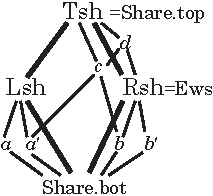
\includegraphics[scale=1.25]{graphics/shares.pdf}}

The \emph{top} share, written \lstinline{Tsh} or
\lstinline{Share.top}, gives total permission: to deallocate any cells
within the footprint of this mapsto, to read, to write.
\[
\begin{array}{ll}
\mathsf{Share.split}~\mathsf{Tsh} = (\mathsf{Lsh},\mathsf{Rsh}) & \\
\mathsf{Share.split}~\mathsf{Lsh} = (a,a')  & \mathsf{Share.split}~\mathsf{Rsh} = (b,b') \\
a'\oplus b = c & \mathrm{lub}(c,\mathsf{Rsh})=a'\oplus \mathsf{Rsh}=d\\
\multicolumn{2}{l}{\forall \mathit{sh}.~\mathsf{writable\_share}~\mathit{sh}~\rightarrow~\mathsf{readable\_share}~\mathit{sh}}\\
\mathsf{writable\_share}~\mathsf{Ews} & \mathsf{readable\_share}~\mathsf{b} \\
\mathsf{writable\_share}~d & \mathsf{readable\_share}~c \\
\mathsf{writable\_share}~\mathsf{Tsh} &  \neg \mathsf{readable\_share}~\mathsf{Lsh} \\
\end{array}
\]
Any share may be split into a \emph{left half} and a \emph{right half}.
The left and right of the top share are given distinguished names
\lstinline{Lsh, Rsh}.

The right-half share of the top share (or any share containing it such
as $d$) is sufficient to grant \emph{write permission} to the data:
``the right share is the write share.''  A thread of execution holding
only \lstinline{Lsh}---or subshares of it such as $a,a'$---can neither
read or write the object, but such shares are not completely useless:
holding any nonempty share prevents other threads from deallocating
the object.

Any subshare of \lstinline{Rsh}, in fact any share that overlaps
 \lstinline{Rsh}, grants \emph{read} permission to the object.
Overlap can be tested using the glb (greatest lower bound) operator.

Whenever \lstinline{(data_at $\mathit{sh}$ t w v)} holds, then the share $\mathit{sh}$
must include at least a read share, thus this gives permission to load
memory at address $v$ to get a value $w$ of type $t$.

To make sure $\mathit{sh}$ has enough permission to write (i.e.,
$\mathsf{Rsh} \subset \mathit{sh}$, we can say \lstinline{writable_share $\mathit{sh}$ : Prop}.

To test whether a share $\mathit{sh}$ is empty or nonempty, use
\lstinline{sepalg.identity $\mathit{sh}$} or
\lstinline{sepalg.nonidentity $\mathit{sh}$}.


Writable extern global variables
come with the ``extern writable share''
\lstinline{Ews}; so does memoryobtained from \lstinline{malloc}.
Stack-allocated addressable locals
come with the ``top share'' \lstinline{Tsh}.
Read-only globals come with
the share \lstinline{Ers}, the ``extern readable share.''

Sequential programs usually have little need of any shares except
the \lstinline{Tsh} and \lstinline{Ews}.  However, many function
specifications can be parameterized over any share (example:
\lstinline{sumarray_spec} on \autopageref{refcard:sumarray-spec});
that kind of
generalized specification makes the functions usable in more contexts.

In C it is undefined to test deallocated pointers for equality or inequalities,
so the Hoare-logic rule for pointer comparison also requires some
permission-share; see \autopageref{refcard:pointer-cmp}.

\chapter{Pointer comparisons}
\label{refcard:pointer-cmp}

In C, if $p$ and $q$ are expressions of type pointer-to-something,
testing \lstinline{$p$=$q$} or \lstinline{$p$!=$q$} is
defined only if: $p$ is \textsc{null}, or points within a
currently allocated object, or points at the end of a currently
allocated object; and similarly for $q$.  Testing
\lstinline{$p$<$q$} (etc.) has even stricter requirements:
$p$ and $q$ must be pointers into the \emph{same} allocated object.

Verifiable C enforces this by creating ``type-checking'' conditions
for the evaluation of such pointer-comparison expressions.
Before reasoning about the result of evaluating expression
\lstinline{$p$==$q$}, you must first prove\newline
\lstinline{tc_expr $\Delta$ (Ebinop Oeq (Etempvar _p (tptr tint)) (Etempvar _q (tptr tint)))},
where \lstinline{tc_expr} is the type-checking condition for that expression.
This simplifies into an entailment
with the current precondition on the left,
and \lstinline{denote_tc_comparable $p$ $q$} on the right.

The \lstinline{entailer(!)} has a solver for such proof goals.
It uses the hint database \lstinline{valid_pointer}.
It relies on spatial terms on the l.h.s. of the entailment,
such as \lstinline{data_at $\pi$ $t$ $v$ $p$} which guarantees
that $p$ points to something.

The file \file{progs/verif\_ptr\_compare.v} illustrates pointer comparisons.

\chapter{Proof of the \textsf{reverse} program}

\emph{Program Logics for Certified Compilers},
Chapter 3
shows a program that reverses a linked list (destructively, in place),
along with a proof of correctness.
(Chapters 2 and 3 available free
\href{http://vst.cs.princeton.edu/download/PLCC-to-chapter-3.pdf#page=20}{here}.)

That proof is based on a general notion of \emph{list segments}.
Here we show a simpler proof that does not use segments, but see
\autoref{refcard:reverse-orig} for proof that corresponds
to Chapters 3 and 27 of PLCC.

The C program is in \file{progs/reverse.c}:
\begin{lstlisting}
struct list {unsigned head; struct list *tail;};

struct list *reverse (struct list *p) {
  struct list *w, *t, *v;
  w = NULL;
  v = p;
  while (v) { t = v->tail; $~$ v->tail = w; $~$ w = v; $~$ v = t; }
  return w;
}
\end{lstlisting}
\vspace{-2ex}

Please open your CoqIDE or Proof General to
\file{progs/verif\_reverse2.v}.
As usual, in \file{progs/verif\_reverse2.v}
we import the clightgen-produced file
\lstinline{reverse.v} and then build \lstinline{CompSpecs} and \lstinline{Vprog}
(see \autopageref{refcard:boilerplate}, \autoref{refcard:compspecs},
\autoref{refcard:global-vars}).

For the \lstinline{struct list} used in this program,
we can define the notion of \emph{linked list}
~~$\listrep{\sigma}{x}{\mathsf{nil}}$
with a recursive definition:

\begin{lstlisting}
Fixpoint listrep (sigma: list val) (x: val) : mpred :=
 match sigma with
 | h::hs => $~$    EX y:val, data_at Tsh t_struct_list (h,y) x  * listrep hs y
 | nil =>  $~~~$   !! (x = nullval) && emp
 end.
\end{lstlisting}

That is, \lstinline{listrep $\sigma$ $x$}
describes a null-terminated linked list starting at pointer $p$,
with permission-share \lstinline{Tsh},
representing the sequence $\sigma$.

The API spec (see also \autoref{refcard:api-spec}) for \lstinline{reverse} is,
\begin{lstlisting}
Definition reverse_spec :=
DECLARE _reverse
 WITH $\sigma$: list val, $p$: val
 PRE  [ _p OF (tptr t_struct_list) ]
  PROP() LOCAL(temp _p $p$)SEP (listrep $\sigma$ $p$)
 POST [ (tptr t_struct_list) ]
  EX $q$:val, PROP() LOCAL(temp _p $q$)SEP (listrep (rev $\sigma$) $q$).
\end{lstlisting}
\vspace{-2ex}
The precondition says
(for $p$ the function parameter)
$\listrep{\sigma}{p}{\mathrm{nil}}$,
and the postcondition says
that (for $q$ the return value)
$\listrep{\mathrm{rev}~\sigma}{q}{\mathrm{nil}}$.

In your IDE, enter the Lemma \lstinline{body_reverse} and
move after the \lstinline{start_function} tactic.
As expected, the precondition for the function-body is
\begin{lstlisting}
PROP() LOCAL(temp _p $p$) SEP(listrep $\sigma$ $p$).
\end{lstlisting}
After \lstinline{forward} through two assignment statements
\lstinline{(w=NULL; v=p;)}
the \lstinline{LOCAL} part also contains
\lstinline{temp _v $p$; temp _w (Vint (Int.repr 0))}.

The loop invariant for the while loop is quite similar to the
one given in PLCC Chapter 3 page 20:
\[\exists \sigma_1,\sigma_2.
~~\sigma=\mathrm{rev}(\sigma_1)\cdot\sigma_2
~\wedge~
\listrep{\sigma_2}{v}{0}
*
\listrep{\sigma_1}{w}{0}
\]
It's
quite typical for loop invariants to existentially quantify
over the values that are different iteration-to-iteration.
We represent this in $\PROP/\LOCAL/\SEP$ notation as,
\begin{lstlisting}
 EX $\sigma_1$: list val, EX $\sigma_2$ : list val, EX $\mathit{w}$: val, EX $\mathit{v}$: val,
   PROP ($\sigma$ = rev $\sigma_1$ ++ $\sigma_2$)
   LOCAL (temp _w $\mathit{w}$; temp _v $\mathit{v}$)
   SEP (listrep $\sigma_1$ $\mathit{w}$; listrep $\sigma_2$ $\mathit{v}$).
\end{lstlisting}

We apply \lstinline{forward_while} with this invariant,
and (as usual) we have four subgoals:
(1) precondition implies loop invariant, (2) loop invariant
implies typechecking of loop-termination test,
(3) loop body preserves invariant, and (4) after the loop.

(1) To prove the precondition implies the loop invariant,
we instantiate $\sigma_1$ with nil
and $\sigma_2$ with $\sigma$;
we instantiate $w$ with \textsc{null} and $v$ with $p$.
But this leaves the goal,
\begin{lstlisting}
ENTAIL $\Delta$, PROP  () LOCAL  (temp _v $p$; temp _w nullval; temp _p $p$)
   SEP  (listrep $\sigma$ $p$)
|-- PROP  ($\sigma$ = rev [] ++ $\sigma$) LOCAL  (temp _w nullval; temp _v $p$)
    SEP  (listrep [] nullval; listrep $\sigma$ $p$)
\end{lstlisting}
\vspace{-3ex}
The \lstinline{PROP} and \lstinline{LOCAL} parts are trivially
solvable by the \lstinline{entailer}.
We can remove the \lstinline{SEP} conjunct
\lstinline{(listrep [] nullval)}
by unfolding that occurrence of \lstinline{listrep},
leaving \lstinline{!!(nullval=nullval)&&emp}.

\vspace{-2ex}
(2) The type-checking condition is not trivial, as it is a pointer
comparison (see \autoref{refcard:pointer-cmp}), but
the \lstinline{entailer!} solves it anyway.

(3) The loop body starts by assuming the \emph{loop invariant}
and the truth of the \emph{loop test}.  Their propositional parts have already
been moved above the line at the comment
\textsf{(* loop body preserves invariant *)}.
That is, \lstinline{HRE: isptr $v$} says that the loop test is true,
and \lstinline{H: $\sigma$ = rev $\sigma_1$ ++ $\sigma_2$} is from the invariant.

The first statement in the loop body, \lstinline{t=v->tail;}
loads from the list cell at $v$.  But our \lstinline{SEP}
assertion for $v$ is,
\lstinline{listrep $\sigma_2$ $v$}.
The assertion
\lstinline{listrep $\sigma_2$ $v$}
is not a \lstinline{data_at} that we can load from.
So we can unfold this occurrence of \lstinline{listrep},
but \emph{still} there is no \lstinline{data_at}
unless we know that $\sigma_2$ is $h::r$ for some $h,r$.

We destruct $\sigma_2$ leaving two cases:
$\sigma_2=\mathsf{nil}$ and
$\sigma_2=h::r$.  The first case is a contradiction---by the
definition of \lstinline{listrep}, we must have $v==\mathsf{nullptr}$,
but that's incompatible with $\mathsf{isptr}(v)$ above the line.

In the second case, we have (below the line)
$\exists y, \ldots$ that binds the value of the
tail-pointer of the first cons cell.  We move that above
the line by \lstinline{Intros y.}

\newthought{Now that the first list-cell is unfolded,}
  it's easy to go \lstinline{forward} through the four commands
  of the loop body.  Now we are
  \textsf{(* at end of loop body, re-establish invariant *).}

We choose values to instantiate the existentials:
\lstinline{Exists (h::$\sigma_1$,r,v,y).}  (Note that
\lstinline{forward_while} has uncurried
the four separate \lstinline{EX} quantifiers
into a single 4-tuple \lstinline{EX}.)  Then
\lstinline{entailer!} leaves two subgoals:
\begin{lstlisting}
______________________________________________(1/2)
rev $\sigma_1$ ++ $h$ :: $r$ = (rev $\sigma_1$ ++ [$h$]) ++ $r$
______________________________________________(2/2)
  listrep $\sigma_1$ $w$ * field_at Tsh t_struct_list [] $(h,w)$ $v$ * listrep $r$ $y$
|-- listrep ($h$ :: $\sigma_1$) $v$ * listrep $r$ $y$
\end{lstlisting}

Indeed, \lstinline{entailer!} always leaves at most two subgoals:
at most one propositional goal, and at most one
cancellation (spatial) goal.
Here, the propositional goal is easily dispatched in the
theory of (Coq) lists.

The second subgoal requires unrolling the r.h.s. list segment,
\label{unroll-the-list}
by unfolding the appropriate instance of \lstinline{listrep}.
Then we appropriately instantiate some existentials,
call on the \emph{entailer!} again, and the goal is solved.

(4) After the loop, we must prove that the loop invariant
\emph{and the negation of the loop-test condition} is a sufficient
precondition for the next statement(s).  In this case,
the next statement is a return; one can \emph{always}
go forward through a return, but now we have to prove
that our current assertion implies the function postcondition.
This is fairly straightfoward.

\chapter{Alternate proof of \textsf{reverse}}
\label{refcard:reverse-orig}

Chapter 27 of PLCC describes a proof of the same list-reverse program,
based on a general theory of list segments.  That proof is shown
in \file{progs/verif\_reverse.v}.

The general theory is in \file{progs/list\_dt.v}.
It accommodates list segments
over any C \lstinline{struct} type, no matter how many fields.
Here, we import
the \lstinline{LsegSpecial} module of that theory,
covering the ``ordinary'' case appropriate for the \lstinline{reverse.c} program.
\begin{lstlisting}
Require Import VST.progs.list_dt. Import LsegSpecial.
\end{lstlisting}

Then we \emph{instantiate} that theory for our particular
\lstinline{struct list} by providing the \lstinline{listspec}
operator with the \emph{names} of the struct (\lstinline{_list})
and the link field (\lstinline{_tail}).
\begin{lstlisting}
Instance LS: listspec _list _tail.
Proof. eapply mk_listspec; reflexivity. Defined.
\end{lstlisting}
All other fields (in this case, just \lstinline{_head}) are
treated as ``data'' fields.

Now, \lstinline{lseg LS $\pi$ $\sigma$ $p$ $q$}
is a list segment starting at pointer $p$,
ending at $q$, with permission-share $\pi$ and contents $\sigma$.

In general, with multiple data fields, the type of $\sigma$
is constructed via \lstinline{reptype} (see \autoref{refcard:reptype}).
In this example, with one data field,
the type of $\sigma$ computes to \lstinline{list val}.

\chapter{Global variables}
\label{refcard:global-vars}

In the C language, ``extern'' global variables
live in the same namespace as local variables, but they
are shadowed by any same-name local definition.
In the C light operational semantics, global variables
live in the same namespace as \emph{addressable} local variables
(both referenced by the expression-abstract-syntax
constructor \lstinline{Evar}),
but in a different namespace from \emph{nonaddressable} locals
(expression-abstract-syntax
constructor \lstinline{Etempvar}).\footnote{This difference in namespace
treatment cannot matter in a program translated by CompCert clightgen from C,
because no as-translated expression will exercise the difference.}

In the program-AST produced by clightgen, globals (and their initializers)
are listed as \lstinline{Gvar}s in the \lstinline{prog_defs}.
These are accessed (automatically) in two ways by the Verifiable C
program logic.  First, their names and types are gathered into
\lstinline{Vprog} as shown on \autopageref{Vprog-page}
(try the Coq command \lstinline{Print Vprog} to see this list).
Second, their initializers are translated into
\lstinline{data_at} conjuncts of separation logic
as part of the \lstinline{main_pre} definition
(see \autopageref{main-pre-page}).

When proving \lstinline{semax_body} for the main
function, the \lstinline{start_function} tactic takes these definitions
from \lstinline{main_pre} and puts them in the precondition
of the function body.  In
some cases this is done using the more-primitive \lstinline{mapsto}
operator\footnote{For example, examine the proof state in
  \file{progs/verif\_reverse.v} immediately after \textsf{start\_function} in \textsf{Lemma body\_main}; and see the conversion to
\textsf{data\_at} done by the \textsf{setup\_globals} lemma in that file.},
in other cases it uses the higher-level (and more standard)
\lstinline{data_at}\footnote{For example,
   examine the proof state in
  \file{progs/verif\_sumarray.v} immediately after \textsf{start\_function} in \textsf{Lemma body\_main}.}.

\ychapter{For loops (special case)}{}
\label{refcard:for}

\newthought{Many for-loops have the form},
~~~\lstinline{ for ($\mathit{init}$; i < $\mathit{hi}$; i++) $\mathit{body}$}
\newline
such that the expression \textit{hi} will evaluate to the same value
every time around the loop.  This upper-bound expression need not
be a literal constant, it just needs to be invariant.

For these loops you can use the tactic,
\begin{lstlisting}
forward_for_simple_bound $n$ (EX $i$:Z, PROP($\vec{P}$) LOCAL($\vec{Q}$) SEP($\vec{R}$)%assert.
forward_for_simple_bound $n$ (EX $i$:Z, EX $x$:$A$, PROP$\ldots$LOCAL$\ldots$SEP$\ldots$)%assert.
\end{lstlisting}
\vspace{-16pt}
where $n$ is the upper bound: a Coq value of type $Z$
such that \textit{hi} will evaluate to $n$.
This tactic generates simpler subgoals than the general \lstinline{forward_for} tactic.

The loop invariant is
\lstinline{(EX $i$:Z, PROP($\vec{P}$) LOCAL($\vec{Q}$) SEP($\vec{R}$))},
where $i$ is the value (in each iteration) of the loop iteration variable
\lstinline{_i}.  You \emph{must} have an existential quantifier for the \emph{value} of the loop-iteration variable.  You \emph{may} have a second $\exists$ for a value of your choice that depends on $i$.

\textbf{You must omit} from $Q$ any mention of the loop iteration variable
\lstinline{_i}.  The tactic will insert the binding \lstinline{temp _i $i$}.
You need not write $i\le\mathit{hi}$ in $P$, the tactic will
insert it.

\newthought{An example} of a for-loop proof is in
\file{progs/verif\_sumarray2.v}.
This is an alternate implementation of \file{progs/sumarray.c}
(see \autoref{refcard:forward-while})
that uses a \lstinline{for} loop instead of a \lstinline{while} loop:
\begin{lstlisting}
unsigned sumarray(unsigned a[], int n) {   /* sumarray2.c */
  int i; unsigned s=0;
  for (i=0; i<n; i++) { s += a[i]; }
  return s;
}
\end{lstlisting}
\vspace{-16pt}
Also see \file{progs/verif\_min.v} for several approaches to the specification/verification of another for-loop.

\ychapter{For loops (general iterators)}{}
\label{refcard:for-general-iter}

{\small
The C-language \textsf{for} loop has the general form,
\lstinline{for ($\mathit{init}$; $\mathit{test}$; $\mathit{incr}$) $\mathit{body}$}.
If your for-loop has an iteration variable that is tested by the $\mathit{test}$
and adjusted by the $\mathit{incr}$, then you can probably use
\lstinline{forward_for}, described in this chapter.  If not,
use \lstinline{forward_loop} (see the next chapter).

Let \textit{Inv} be the loop invariant, established by the
initializer and preserved
by the body-plus-increment.  Let \textit{PreInc} be
the assertion just before the increment.
Both \textit{Inv} and \textit{PreInc}
have type $A\rightarrow\mathsf{environ}\rightarrow\mathsf{mpred}$,
where $A$ is the Coq type of the abstract values carried by your
iteraction variable; typically this is just \lstinline{Z}.

\textit{Post} is the join-postcondition of the loop;
you don't need to provide it if \emph{either} (1) there are
no \lstinline{break} statements in the loop, or (2)
the postcondition is already provided in your proof context
(typically because a close-brace follows the entire loop).
Depending on whether you need \emph{Post}, verify the loop with,

\noindent\lstinline{forward_for $\mathit{Inv}$.}\qquad if your loop has no \lstinline{break} or \lstinline{continue} statements; or\newline
\noindent\lstinline{forward_for $\mathit{Inv}$ continue: $\mathit{PreInc}$.}\qquad if no \lstinline{break} statements; or\newline
\lstinline{forward_for $\mathit{Inv}$ continue: $\mathit{PreInc}$ break: $\mathit{Post}$.}

This is demonstrated in
\lstinline{body_sumarray_alt} from
\file{progs/verif\_sumarray2.v}.

\begin{lstlisting}
unsigned sumarray(unsigned a[], int n) {
  int i; unsigned s;
  s=0;
  for (i=0;
    /* $\mathit{Inv}:$ loop invariant */
            i<n; i++) {
    s += a[i];
    /* $\mathit{PreInc}:$ pre-increment invariant */
  }
  /* $\mathit{Post}:$ loop postcondition */
  return s;
}
\end{lstlisting}
}

\ychapter{Loops (fully general)}{}
\label{refcard:for-general}

The C-language \textsf{for} loop has the general form,
\lstinline{for ($\mathit{init}$; $\mathit{test}$; $\mathit{incr}$) $\mathit{body}$}.

The C-language \textsf{while} loop with \lstinline{break} and \lstinline{continue} is equivalent to a \textsf{for} loop with empty $\mathit{init}$ and
$\mathit{incr}$.

The C-language infinite-loop, written \ \ \lstinline{for(;;)$c$}\ \ 
or \ \ \lstinline{while(1)$c$}\ \  is also a form of the for-loop.

The most general tactic for proving any of these loops is,\newline
\lstinline{forward_loop $\mathit{Inv}$ continue: $\mathit{PreInc}$ break: $\mathit{Post}$}.

The assertion $\mathit{Inv}: \mathsf{environ->mpred}$ is the loop invariant.\newline
$\mathit{PreInc}: \mathsf{environ->mpred}$ is the invariant just before the $\mathit{incr}$.\newline
The assertion $\mathit{Post}: \mathsf{environ->mpred}$ is the postcondition
of the loop.

If your $\mathit{incr}$ is empty (or Sskip),
or if the $\mathit{body}$ has no \lstinline{continue} statements,
you can omit \ \ \lstinline{continue: $\mathit{PreInc}$}.

If your postcondition is already fully determined (POSTCOND contains no unification variables), then you can omit \ \ \lstinline{break: $\mathit{Post}$}.

If you're not sure whether to omit the \lstinline{break:} or \lstinline{continue:} assertions, just try \lstinline{forward_loop $\mathit{Inv}$} without them, and Floyd will advise you.


\chapter{Manipulating preconditions}
In some cases you cannot go \lstinline{forward} until the precondition
has a certain form.  For example, to go \lstinline{forward}
through \lstinline{t=v->tail;} there must be a
\lstinline{data_at} or \lstinline{field_at} in the \lstinline{SEP}
clause of the precondition that gives a value for
\lstinline{_tail} field of \lstinline{t}.
As
\autopageref{unroll-the-list}
describes, a listrep can be unfolded
to expose such a \lstinline{SEP} conjunct.

Faced with the proof goal,\hfill
$\mathsf{semax}~~\Delta~~(\PROP(\vec{P}) \LOCAL(\vec{Q}) \SEP(\vec{R}))~~c~~\mathit{Post}$
where $\PROP(\vec{P}) \LOCAL(\vec{Q}) \SEP(\vec{R})$ does not match
the requirements for forward symbolic execution,
you have several choices:
\begin{itemize}
\item Use the rule of consequence explicitly:\newline
\lstinline|apply semax_pre with $\PROP(\vec{P'}) \LOCAL(\vec{Q'}) \SEP(\vec{R'})$|,\newline
then prove $\mathsf{ENTAIL}~\Delta,~\vec{P};\vec{Q};\vec{R}\vdash\vec{P'};\vec{Q'};\vec{R'}$.
\item Use the rule of consequence implicitly,
by using tactics (\autopageref{refcard:manip}) that modify the precondition.
\item Do rewriting in the precondition, either directly by the
standard \lstinline{rewrite} and \lstinline{change} tactics,
or by \lstinline{normalize} (\autopageref{refcard:normalize}).
\item Extract propositions and existentials from the precondition,
by using \lstinline{Intros} (\autopageref{refcard:intros})
or \lstinline{normalize}.
\item Flatten stars into semicolons, in the \lstinline{SEP} clause,
 by \lstinline{Intros}.
\item Use the freezer (\autopageref{freezer}) to temporarily ``frame away'' spatial conjuncts.
\end{itemize}

\newpage
\newthought{Tactics for manipulating preconditions.}
\label{refcard:manip}
In many of these tactics we select specific conjucts from the
\SEP{} items, that is, the semicolon-separated list of
separating conjuncts.  These tactic refer to the list
by zero-based position number, 0,1,2,\ldots.

For example, suppose the goal is a \lstinline{semax}
or entailment containing \lstinline|PROP($\vec{P}$)LOCAL($\vec{Q}$)SEP(a;b;c;d;e;f;g;h;i;j).|
Then:

\sbox{\mybox}{\emph{results in}}
\begin{description}\setlength{\itemsep}{2ex}
\item[$\mathsf{focus\_SEP}~i~j~k$.]
Bring items \#$i,j,k$ to the front of the \SEP{} list.
\begin{lstlisting}
focus_SEP 5.  $~~~\usebox{\mybox}~$PROP($\vec{P}$)LOCAL($\vec{Q}$)SEP(f;a;b;c;d;e;g;h;i;j).
focus_SEP 0.  $~~~\usebox{\mybox}~$PROP($\vec{P}$)LOCAL($\vec{Q}$)SEP(a;b;c;d;e;f;g;h;i;j).
focus_SEP 1 3. $~\usebox{\mybox}~$PROP($\vec{P}$)LOCAL($\vec{Q}$)SEP(b;d;a;c;e;f;g;h;i;j)
focus_SEP 3 1. $~\usebox{\mybox}~$PROP($\vec{P}$)LOCAL($\vec{Q}$)SEP(d;b;a;c;e;f;g;h;i;j)
\end{lstlisting}
\item[$\mathsf{gather\_SEP}~i~j~k$.]
Bring items \#$i,j,k$ to the front of the \SEP{} list
and conjoin them into a single element.
\begin{lstlisting}
gather_SEP 5.  $~~~\usebox{\mybox}~$PROP($\vec{P}$)LOCAL($\vec{Q}$)SEP(f;a;b;c;d;e;g;h;i;j).
gather_SEP 1 3. $~\usebox{\mybox}~$PROP($\vec{P}$)LOCAL($\vec{Q}$)SEP(b*d;a;c;e;f;g;h;i;j)
gather_SEP 3 1. $~\usebox{\mybox}~$PROP($\vec{P}$)LOCAL($\vec{Q}$)SEP(d*b;a;c;e;f;g;h;i;j)
\end{lstlisting}
\item[$\mathsf{replace\_SEP}~i~R$.]
Replace the $i$th element the \SEP{} list
with the assertion $R$, and leave a subgoal to prove.
\begin{lstlisting}
replace_SEP 3 R.  $~~~\usebox{\mybox}~$PROP($\vec{P}$)LOCAL($\vec{Q}$)SEP(a;b;c;$R$;e;f;g;h;i;j).
\end{lstlisting}
with subgoal~~~ $\PROP(\vec{P})\LOCAL(\vec{Q})\SEP(\textsf{d}) \vdash R$.
\item[$\mathsf{replace\_in\_pre}~S~S'$.]
Replace $S$ with $S'$ anywhere it occurs in the precondition
then leave
$(\vec{P};\vec{Q};\vec{R}) \vdash (\vec{P};\vec{Q};\vec{R})[S'/S]$
as a subgoal.
\item[$\mathsf{frame\_SEP}~i~j~k.$]
Apply the frame rule, keeping only
elements $i,j,k$ of the \SEP{} list.  See \autoref{refcard:frame}.
\end{description}

\ychapter{The Frame rule}{}
\label{refcard:frame}

Separation Logic supports the Frame rule,
\[\inference[Frame]{\triple{P}{c}{Q}}{\triple{P*F}{c}{Q*F}}\]

In VST, we recommend you use the \lstinline{freeze} tactic instead; see \autoref{freezer}.  But if you really want to use the frame rule, here is how.

Suppose you have the proof goal,
\begin{lstlisting}
semax $\Delta$ $\PROP(\vec{P})\LOCAL(\vec{Q})\SEP(R_0;R_1;R_2)~$ $(c_1;c_2);c_3$ $~\mathit{Post}$
\end{lstlisting}
and suppose you want to ``frame out'' $R_1$ for the duration of
$c_1;c_2$, and have it back again for $c_3$.

First, you grab the first 2 statements using the tactic, \newline
\lstinline{first_N_statements 2%nat}.  (This works the same regardless of the
  nesting structure of the semicolons; it reassociates as needed.)

This leaves the two subgoals,
\begin{lstlisting}
semax $\Delta$ $\PROP(\vec{P})\LOCAL(\vec{Q})\SEP(R_0;R_1;R_2)~$ $c_1;c_2$ $~\mathsf{(normal\_ret\_assert ?88)}$
semax $\Delta$ $~\mathsf{?88}~$ $c_3$ $~\mathit{Post}$
\end{lstlisting}

In the first subgoal, do \lstinline{frame_SEP$~$0 2} to retain only $R_0;R_2$.
\begin{lstlisting}
semax $\Delta$ $\PROP(\vec{P})\LOCAL(\vec{Q})\SEP(R_0;R_2)~$ $c_1;c_2$ $~\ldots$
\end{lstlisting}
Now you'll see that (in the precondition of the second subgoal)
the unification variable $\mathsf{?88}$ has been
instantiated in such a way that $R_1$ is added back in.
Now you can prove the two subgoals, in order.


\ychapter{The Freezer (\textsf{freeze,thaw})}{}
\label{freezer}
Suppose you have the proof goal,
\begin{lstlisting}
semax $\Delta$ $\PROP(\vec{P})\LOCAL(\vec{Q})\SEP(R_0;R_1;R_2)~$ $c_1;c_2;c_3$ $~\mathit{Post}$
\end{lstlisting}
and suppose you want to ``frame out'' $R_0$ and $R_2$ for the duration of
$c_1;c_2$, and have them back again for $c_3$.
Instead of using the frame rule, you can use the freezer.

First, say \lstinline{freeze FR1 := R0 R2.}\newline
The name \lstinline{FR1} is up to you; R0 and R2 must be patterns
(perhaps with underscores,
for example \lstinline{(data_at _$~$_$~$_$~$p)}) 
that match conjuncts from the SEP clause.

Now the proof goal looks like this:
\begin{lstlisting}
semax $\Delta$ $\PROP(\vec{P})\LOCAL(\vec{Q})\SEP(\mbox{\textsc{frzl}}~\mathsf{FR1};~ R_1)~$ $c_1;c_2;c_3$ $~\mathit{Post}$\end{lstlisting}
with a definition ~ \lstinline{FR1 := $\ldots$} ~ above the line.

You can also write \qquad
$\mathit{freeze}\ F\ \mathsf{:=}\ \mathsf{-}\ \mathit{pattern}_1  ~\mathit{pattern}_2 \ldots \mathit{pattern}_n$ \newline
to freeze into $F$ every conjunct \emph{except} those that match the patterns.


Proceed forward through $c_1$ and $c_2$; then you can give the command
\lstinline{thaw FR1} that unfolds (and clears) the FR1 definition.

Freezers can coexist and be arbitrarily nested, and be thawed independently; freezer-conjuncts participate in \lstinline{cancel} and other separation-logic operations.

\ychapter{32-bit Integers}{(\file{compcert/lib/Integers.v})}
\label{refcard:32bit}

The VST program logic uses CompCert's 32-bit integer type.

\begin{lstlisting}
Inductive comparison := Ceq | Cne | Clt | Cle | Cgt | Cge.
Int.wordsize: nat = 32.
Int.modulus : Z = $2^{32}$.
Int.max_unsigned : Z = $2^{32}-1$.
Int.max_signed : Z = $2^{31}-1$.
Int.min_signed : Z = $-2^{31}$.

Int.int : Type.
Int.unsigned : int -> Z.
Int.signed : int -> Z.
Int.repr : Z -> int.

Int.zero := Int.repr 0.

$\mbox{\textbf{(* Operators of type int\(\rightarrow\)int\(\rightarrow\)bool *)}}$
Int.eq $$ Int.lt $$ Int.ltu $$ Int.cmp(c:comparison) $$ Int.cmpu(c:comparison)

$\mbox{\textbf{(* Operators of type int\(\rightarrow\)int *)}}$
Int.neg $$ Int.not

$\mbox{\textbf{(* Operators of type int\(\rightarrow\)int\(\rightarrow\)int *)}}$
Int.add $$ Int.sub $$  Int.mul $$  Int.divs $$  Int.mods $$  Int.divu $$  Int.modu
Int.and $$ Int.or $$ Int.xor $$ Int.shl $$ Int.shru $$ Int.shr $$ Int.rol $$ Int.ror $$  Int.rolm

Lemma eq_dec: forall (x y: int), {x = y} + {x <> y}.
Theorem unsigned_range: forall i, 0 <= unsigned i < modulus.
Theorem unsigned_range_2:  forall i, 0 <= unsigned i <= max_unsigned.
Theorem signed_range:  forall i, min_signed <= signed i <= max_signed.
Theorem repr_unsigned:  forall i, repr (unsigned i) = i.
Lemma repr_signed:  forall i, repr (signed i) = i.
Theorem unsigned_repr:
   forall z, 0 <= z <= max_unsigned -> unsigned (repr z) = z.
Theorem signed_repr:
  forall z, min_signed <= z <= max_signed -> signed (repr z) = z.
Theorem signed_eq_unsigned:
  forall x, unsigned x <= max_signed -> signed x = unsigned x.

Theorem unsigned_zero: unsigned zero = 0.
Theorem unsigned_one: unsigned one = 1.
Theorem signed_zero: signed zero = 0.

Theorem eq_sym:  forall x y, eq x y = eq y x.
Theorem eq_spec: forall (x y: int), if eq x y then x = y else x <> y.
Theorem eq_true: forall x, eq x x = true.
Theorem eq_false: forall x y, x <> y -> eq x y = false.

Theorem add_unsigned: forall x y, add x y = repr (unsigned x + unsigned y).
Theorem add_signed: forall x y, add x y = repr (signed x + signed y).
Theorem add_commut: forall x y, add x y = add y x.
Theorem add_zero: forall x, add x zero = x.
Theorem add_zero_l: forall x, add zero x = x.
Theorem add_assoc: forall x y z, add (add x y) z = add x (add y z).

Theorem neg_repr: forall z, neg (repr z) = repr (-z).
Theorem neg_zero: neg zero = zero.
Theorem neg_involutive: forall x, neg (neg x) = x.
Theorem neg_add_distr: forall x y, neg(add x y) = add (neg x) (neg y).

Theorem sub_zero_l: forall x, sub x zero = x.
Theorem sub_zero_r: forall x, sub zero x = neg x.
Theorem sub_add_opp: forall x y, sub x y = add x (neg y).
Theorem sub_idem: forall x, sub x x = zero.
Theorem sub_add_l: forall x y z, sub (add x y) z = add (sub x z) y.
Theorem sub_add_r: forall x y z, sub x (add y z) = add (sub x z) (neg y).
Theorem sub_shifted: forall x y z, sub (add x z) (add y z) = sub x y.
Theorem sub_signed:  forall x y, sub x y = repr (signed x - signed y).

Theorem mul_commut: forall x y, mul x y = mul y x.
Theorem mul_zero: forall x, mul x zero = zero.
Theorem mul_one: forall x, mul x one = x.
Theorem mul_assoc: forall x y z, mul (mul x y) z = mul x (mul y z).
Theorem mul_add_distr_l: forall x y z, mul (add x y) z = add (mul x z) (mul y z).
Theorem mul_signed: forall x y, mul x y = repr (signed x * signed y).
\end{lstlisting}
and many more axioms for the bitwise operators, shift operators,
signed/unsigned division and mod operators.

\chapter{CompCert C abstract syntax}

The CompCert verified C compiler translates standard C source programs
into an abstract syntax for \emph{CompCert C},
and then translates that into abstract syntax
for \emph{C light}.
Then VST Separation Logic is applied to the C light abstract syntax.
C light programs proved correct using the VST separation logic
can then be compiled (by CompCert) to assembly language.

C light syntax is defined by these Coq files from CompCert:

\begin{description}
\item[Integers.]  32-bit (and 8-bit, 16-bit, 64-bit) signed/unsigned integers.
\item[Floats.]  IEEE floating point numbers.
\item[Values.]  The \lstinline|val| type: integer + float + pointer + undefined.
\item[AST.]  Generic support for abstract syntax.
\item[Ctypes.]  C-language types and structure-field-offset computations.
\item[Clight.]  C-light expressions, statements, and functions.
\end{description}

You will see C light abstract syntax constructors
in the Hoare triples (\lstinline{semax}) that you are verifying.
We summarize the constructors here.

\begin{lstlisting}
Inductive expr : Type :=
(* 1$~$  *) $~~~$   | Econst_int: int -> type -> expr
(* 1.0 *)   $~$ | Econst_float: float -> type -> expr  (* double precision *)
(* 1.0f0 *)    | Econst_single: float -> type -> expr (* single precision *)
(* 1L  *)  $~~$  | Econst_long: int64 -> type -> expr
(* x   *) $~~~~$   | Evar: ident -> type -> expr
(* x   *) $~~~~$   | Etempvar: ident -> type -> expr
(* *e  *) $~~~$   | Ederef: expr -> type -> expr
(* &e  *) $~~$   | Eaddrof: expr -> type -> expr
(* ~e  *) $~~$   | Eunop: unary_operation -> expr -> type -> expr
(* e+e *) $~$   | Ebinop: binary_operation -> expr -> expr -> type -> expr
(* (int)e *) | Ecast: expr -> type -> expr
(* e.f *) $~~$ | Efield: expr -> ident -> type -> expr.

Inductive unary_operation := Onotbool | Onotint | Oneg | Oabsfloat.
Inductive binary_operation := Oadd | Osub | Omul | Odiv | Omod
 | Oand | Oor | Oxor | Oshl | Oeq | One | Olt | Ogt | Ole | Oge.

Inductive statement : Type :=
(* /**/;*)  $~~~~~~$ | Sskip : statement
(* $E_1$=$E_2$; *)$~\,~$  | Sassign : expr -> expr -> statement (* memory store *)
(* $x$=$E$; *)$~~~~~~$  | Sset : ident -> expr -> statement   (* tempvar assign *)
(* $x$=$f$(...); *)$~\,$  | Scall: option ident -> expr -> list expr -> statement
(* $x$=$b$(...); *)$~\,$ | Sbuiltin: option ident -> external_function -> typelist ->
$\hspace{3in}$list expr -> statement
(* $s_1$; $s_2$ *)$~~~~~~$ | Ssequence : statement -> statement -> statement
(* if() else {} *) | Sifthenelse : expr  -> statement -> statement -> statement
(* for (;;$s_2$) $s_1$ *) | Sloop: statement -> statement -> statement
(* break; *)$~~~~~~$  | Sbreak : statement
(* continue; *)$~~$ | Scontinue : statement
(* return $E$; *)$~~$ | Sreturn : option expr -> statement
$~~~~~~~~~~~~~~~$  | Sswitch : expr -> labeled_statements -> statement
$~~~~~~~~~~~~~~~$  | Slabel : label -> statement -> statement
$~~~~~~~~~~~~~~~$  | Sgoto : label -> statement.
\end{lstlisting}

\chapter{C light semantics}

The operational semantics of C light statements and expressions
is given in \file{compcert/cfrontend/Clight.v}.  We do not expose
these semantics \emph{directly} to the user of Verifiable C.
Instead, the \emph{statement} semantics is reformulated
as \lstinline{semax}, an axiomatic (Hoare-logic style) semantics.
The \emph{expression} semantics is reformulated in
\file{veric/expr.v} and \file{veric/Cop2.v} as
a \emph{computational\footnote{that is, defined by \textsf{Fixpoint} instead of
    by \textsf{Inductive}.}
big-step evaluation semantics}.
In each case, a soundness proof relates the Verifiable C semantics
to the CompCert Clight semantics.

Rules for \lstinline{semax} are given in
\file{veric/SeparationLogic.v}---but you rarely use
these rules directly.  Instead, derived lemmas regarding
\lstinline{semax} are proved in \file{floyd/*.v} and
Floyd's \lstinline{forward} tactic applies them (semi)automatically.

The following functions (from \file{veric/expr.v}) define
expression evaluation:
\begin{lstlisting}
eval_id {CS: compspecs} (id: ident) : environ -> val.
          (* evaluate a tempvar *)
eval_var {CS: compspecs} (id: ident) (ty: type) : environ -> val.
          (* evaluate an lvar or gvar, addressable local or global variable *)
eval_cast (t t': type) (v: val) : val.
      (* cast value v from type t to type t', but beware! There are
        $\mathit{three}$ types involved, including native type of v. *)
eval_unop (op: unary_operation) (t1 : type) (v1 : val) : val.
eval_binop{CS:compspecs} (op:binary_operation) (t1 t2: type) (v1 v2: val): val.
eval_lvalue {CS: compspecs} (e: expr) : environ -> val.
     (* evalue an $l$-expression, one that denotes a loadable/storable place*)
eval_expr {CS: compspecs} (e: expr) : environ -> val.
     (* evalue an $r$-expression, one that is not storable *)\end{lstlisting}

The \emph{environ} argument is for looking up the values of
local and global variables.  However, in most cases where
Verifiable C users see \lstinline{eval_lvalue}
or \lstinline{eval_expr}---in subgoals generated by the
\lstinline{forward} tactic---all the variables have already been
substituted by values.  Thus the environment is not needed.

The expression-evaluation functions call upon several helper
functions from \file{veric/Cop2.v}:

\begin{lstlisting}
sem_cast: type -> type -> val -> option val.
sem_cast_* (* several helper functions for sem_cast *)
bool_val: type -> val -> option bool.
bool_val_*: (* helper functions *)
sem_notbool: type -> val -> option val.
sem_neg: type -> val -> option val.
sem_sub {CS: compspecs}: type -> type -> val -> val -> option val.
sem_sub_*: (* helper functions *)
sem_add {CS: compspecs}: type -> type -> val -> val -> option val.
sem_add_*: (* helper functions *)
sem_mul: type -> type -> val -> val -> option val.
sem_div: type -> type -> val -> val -> option val.
sem_mod: type -> type -> val -> val -> option val.
sem_and: type -> type -> val -> val -> option val.
sem_or:  type -> type -> val -> val -> option val.
sem_xor: type -> type -> val -> val -> option val.
sem_shl: type -> type -> val -> val -> option val.
sem_shr: type -> type -> val -> val -> option val.
sem_cmp: comparison -> type -> type -> (...) -> val -> val -> option val.
sem_unary_operation: unary_operation -> type -> val -> option val.
sem_binary_operation {CS: compspecs}:
   binary_operation -> type -> type -> mem -> val -> val -> option val.
\end{lstlisting}
The details are not so important to remember.  The main point is
that Coq expressions of the form \lstinline{sem_}\ldots
\emph{should} simplify away, provided that their arguments
are instantiated with concrete operators,
concrete constructors \lstinline{Vint/Vptr/Vfloat},
and concrete C types.
The \emph{int} values (etc.) carried inside
\lstinline{Vint/Vptr/Vfloat}
\emph{do not} need to be concrete: they can be Coq variables.
This is the essence of proof by symbolic execution.


\chapter{Splitting arrays}
\label{refcard:split-array}
Consider this example, from the \lstinline{main}
function of \file{progs/verif\_sumarray2.v}:
%$\mathit{sh}$: share
%$k$: Z
%$\mathit{al}$: list val
%$p$: val
\begin{lstlisting}
data_at $\mathit{sh}$ (tarray tuint $k$) $\mathit{al}$ $p$ : mpred
\end{lstlisting}
\vspace{-\baselineskip}
The \lstinline{data_at} predicate here says that in memory
starting at address $p$ there is an array of $k$ slots
containing, respectively, the elements of the sequence
$\mathit{al}$.

Suppose we have a function \lstinline{sumarray(unsigned a[], int n)}
that takes an array of length $n$, and we apply it to
a ``slice'' of $p$:  \lstinline{sumarray(p+i,k-i);}
where $0 \le i \le k$.
The precondition of the \lstinline{sumarray}
funspec has \lstinline{data_at $\mathit{sh}$ (tarray tint $n$) $\mathit{bl}$ $a$}.  In this case, we would like $a=\&(p[i])$, $n=k-j$, and
$\mathit{bl}=$ the sublist of $\mathit{al}$ from $i$ to $k-1$.

To prove this function-call by \lstinline{forward_call}, we must
split up\linebreak
\lstinline{(data_at $\mathit{sh}$ (tarray tint $k$) $\mathit{al}$ $p$)}
into two conjuncts:\newline
\lstinline{(data_at $\mathit{sh}$ (tarray tint $i$) (sublist 0 $i$ $\mathit{al}$) $p$  *}\newline
\hspace*{1in} \lstinline{data_at $\mathit{sh}$ (tarray tuint $(k-i)$) (sublist $i$ $k$ $\mathit{al}$) $q$)},\newline
where $q$ is the pointer to the array slice beginning at address $p+i$.
We write this as,
\lstinline{$q=$ field_address0 (tarray tint $k$) [ArraySubsc $i$] $p$.}
That is, given a pointer $p$ to a data structure described
by \lstinline{(tarray tint $k$)},
calculate the \emph{address} for subscripting the $i$th element.
(See \autoref{refcard:field-address})

As shown in the \lstinline{body_main} proof in
\file{progs/verif\_sumarray2.v},
the lemma \lstinline{split_array} proves the equivalence of
these two predicates, using the VST-Floyd lemma
\lstinline{split2_data_at_Tarray}.  Then the \lstinline{data_at $\ldots$ $q$}
  predicate can satisfy the precondition of \lstinline{sumarray},
  while the $p$ slice will be part of the ``frame'' for the function
  call.

See also: \lstinline{split3_data_at_Tarray}.
\chapter{sublist}
\label{refcard:sublist}

\emph{Since VST 2.6, we recommend using the new \emph{\lstinline{list_solve}}
and \emph{\lstinline{list_simplify}} tactics, described in
\autoref{refcard:list_solve} and \autoref{refcard:list_solve-advanced}.
Using \textbf{autorewrite with sublist} is less efficient,
and in certain corner cases, can turn provable goals into unprovable goals.}

\autoref{refcard:split-array} explained that we often need
to reason about slices of arrays whose contents are sublists of lists.
For that we have a function \lstinline{sublist $i$ $j$ $l$}
which makes a new list out of the elements $i\ldots j-1$ of
list $l$.

To simplify expressions involving,
\lstinline{sublist},
\lstinline{++},
\lstinline{map},
\lstinline{Zlength},
\lstinline{Znth},
and \lstinline{list_repeat},
use \textbf{autorewrite with sublist}.

Often, you find equations ``above the line'' of the form,
\begin{lstlisting}
H: n = Zlength (map Vint (map Int.repr contents))
\end{lstlisting}
\vspace{-\baselineskip}
You may find it useful to do \lstinline{autorewrite with sublist in *|-}
to change this to \lstinline{n=Zlength contents} before proceeding
with \lstinline{(autorewrite with sublist)} below the line.

These rules comprise the \lstinline{sublist} \emph{rewrite database}:

\begin{lstlisting}
sublist_nil':  $i=j$ -> sublist $i$ $j$ $l$ = [$\,$].
app_nil_l: [$\,$] ++ $l$ = $l$.
app_nil_r: $l$ ++ [$\,$] = $l$.
Zlength_rev:  Zlength (rev $l$) = Zlength $l$.
sublist_rejoin': $0 \le i \le j = j' \le k \le \mathsf{Zlength}\,l$ ->
       sublist $i$ $j$ $l$ ++ sublist $j'$ $k$ $l$ = sublist $i$ $k$ $l$.
subsub1: $a-(a-b)=b$.
Znth_list_repeat_inrange: $0 \le i \le n$ -> Znth $i$ (list_repeat (Z.to_nat $n$) a) = a.
Zlength_cons: Zlength ($a$::$l$) = Z.succ (Zlength $l$).
Zlength_nil: Zlength [$\,$] = 0.
Zlength_app: Zlength ($l$ ++ $l'$) = Zlength $l$ ++ Zlength $l'$.
Zlength_map: Zlength (map $f$ $l$) = Zlength $l$.
list_repeat_0: list_repeat (Z.to_nat 0) = [$\,$].
Zlength_list_repeat: $0\le n$ -> Zlength (list_repeat (Z.to_nat $n$)) = $n$.
Zlength_sublist: $0 \le i \le j \le \mathsf{Zlength}\,l$ -> Zlength(sublist $i$ $j$ $l$) = $j-i$.
sublist_sublist: $ 0 \le m$ -> $0 \le k \le i \le j - m$ ->
       sublist $k$ $i$ (sublist $m$ $j$ $l$) = sublist ($k+m$) ($i+ m$) $l$.
sublist_app1: $0 \le i \le j \le \mathsf{Zlength}~l$ -> sublist $i$ $j$ ($l$ ++ $l'$) = sublist $i$ $j$ $l$.
sublist_app2: $0 \le \mathsf{Zlength}\,l \le i$ ->
      sublist $i$ $j$ ($l$ ++ $l'$) = sublist $(i - \mathsf{Zlength}\,l)$ $(j - \mathsf{Zlength}\,l)$ $l'$.
sublist_list_repeat: $0 \le i \le j \le k$ ->
       sublist $i$ $j$ (list_repeat (Z.to_nat $k$) $v$) = list_repeat (Z.to_nat $(j - i)$) $v$.
sublist_same: $i=0$ -> $j=\mathsf{Zlength}\,l$ -> sublist $i$ $j$ $l$ = $l$.
app_Znth1:  $i < \mathsf{Zlength}\, l$ -> Znth $i$ ($l$ ++ $l'$) = Znth $i$ $l$.
app_Znth2:  $i \ge \mathsf{Zlength}\, l$ -> Znth $i$ ($l$ ++ $l'$) = Znth $i-\mathsf{Zlength}\,l$ $l'$.
Znth_sublist: $0 \le i$ -> $0 \le j < k-i$ -> Znth $j$ (sublist $i$ $k$ $l$) = Znth ($j$ + $i$) $l$.
\end{lstlisting}
\vspace{-\baselineskip}
along with miscellaneous \lstinline{Z} arithmetic:
\[
\begin{array}{c}
n-0=n \quad 0+n=n \quad n+0=n \quad n \le m \rightarrow \mathrm{max}(n,m) = m\\
\quad n + m - n = m
\quad n + m - m = n
\quad m - n + n = m
\quad n-n=0\\
\quad n + m - (n + p) = m - p \qquad \mathrm{et cetera.}
\end{array}
\]

\chapter{list\_solve}
\label{refcard:list_solve}

One often needs to prove goals about lists.
\lstinline{list_solve} is a convenient solver for many practical proof goals involving lists.

\lstinline{list_solve} supports operators:
\lstinline{Zlength},
\lstinline{Znth},
\lstinline{nil} (\lstinline{[]}),
\lstinline{cons} (\lstinline{::}),
\lstinline{Zrepeat},
\lstinline{app} (\lstinline{++}),
\lstinline{upd_Znth},
\lstinline{sublist}, and
\lstinline{map}.

\lstinline{list_solve} supports four kinds of typical proof goals:
\begin{itemize}
    \item linear arithmetic involving lengths of lists,
\begin{lstlisting}
  e.g. Zlength ($l$ ++ $l'$) >= Zlength $l$;
\end{lstlisting}
  \item goal involving nth elements of lists (not limited to equality),
\begin{lstlisting}
  e.g. Znth $i$ ($l$ ++ $l'$) = Znth $i$ $l$;
\end{lstlisting}
  \item equality of lists,
\begin{lstlisting}
  e.g. $l_1$ ++ $l_2$ = $l_3$ ++ $l_4$;
\end{lstlisting}
  \item entailment of array contents,
\begin{lstlisting}
  e.g. data_at $sh$ (tarray $\tau$ $n$) ($l_1$ ++ $l_2$) $p$ |--
         data_at $sh$ (tarray $\tau$ $n$) ($l_3$ ++ $l_4$) $p$.
\end{lstlisting}
\end{itemize}

The way that \lstinline{list_solve} supports assumptions in the following forms,
is to interpret them as quantified properties:
\begin{itemize}
    \item \lstinline{$l$ = $l'$} is replaced by
      \lstinline{Zlength $l$ = Zlength $l'$ /\ forall $i$, $0 \le i < \mathsf{Zlength}\ l$ -> Znth $i$ $l$ = Znth $i$ $l'$}.
    \item \lstinline{In $x$ $l$} is replaced by
      \lstinline{exists $i$, $0 \le i < \mathsf{Zlength}\ l$ /\ $x$ = Znth $i$ $l$}.
    \item \lstinline{~In $x$ $l$} is replaced by
      \lstinline{forall $i$, $0 \le i < \mathsf{Zlength}\ l$ -> $x$ $\neq$ Znth $i$ $l$}.
    \item \lstinline{sorted ($\le$) $l$} is replaced by
      \lstinline{forall $i$ $j$, $0 \le i \le j < \mathsf{Zlength}\ l$ -> $\hspace{80pt}$ ${}$ $\mathsf{Znth}\ i\ l\le \mathsf{Znth}\ j\ l$}.
    % \item \lstinline{Sorted $l$} (\lstinline{Sorted} is defined in \lstinline{Coq.Sorting.Sorted}) is replaced by
    %   \lstinline{forall $i$ $j$, $0 \le i \le j$ /\ $j < \mathsf{Zlength}\ l$ -> Znth $i$ $l$ <= Znth $j$ $l$}.
\end{itemize}

The theory of lists with concatenation and nth-element is known to be undecidable.%
\footnote{The reason is that an element may have relationship with other elements in the same list, directly or indirectly, and that leads to complicated deduction..
For example, \scantokens{\lstinline{sublist $1$ (Zlength $l$) $l$ =} \lstinline{sublist $0$ (Zlength $l$ - 1) $l$}}
indicates \scantokens{\lstinline{Znth $i$ $l$ = Znth $(i+1)$ $l$}} for every $i$ and so all the elements in $l$ are equal.
Such kind of reasoning relies on induction and is hard to automate.
Also see Aaron R. Bradley, Zohar Manna, and Henny B. Sipma, \emph{What’s Decidable About Arrays?}, Lecture Notes in Computer Science, vol 3855. Springer, Berlin, Heidelberg, 2006.
}
So \lstinline{list_solve} has such restriction that when
  encountering quantified properties like
  \lstinline{forall $i$, P (Znth $i$ $l$) (Znth $(i+k)$ $l$)},
it asks user to prove $k=0$ if it cannot prove it automatically.
If $k=0$ is not provable, \lstinline{list_solve} does not support this goal.
User might need to perform an induction before using \lstinline{list_solve}.

\lstinline{list_simplify} is an alternate tactic for \lstinline{list_solve}, like \lstinline{ring_simplify} to \lstinline{ring}.
It performs transformations in the same way as \lstinline{list_solve},
  and solves the goal if \lstinline{list_solve} can solve,
  but leaves the unsolved goals to the user,
so you may solve these goals by hand or figure out why the goal is not solved.
\lstinline{list_simplify} will not change a provable goal into unprovable goals.

\chapter{list\_solve (advanced)}
\label{refcard:list_solve-advanced}
You can enhance \lstinline{list_solve} by adding new rules.

\paragraph{Adding a macro} A macro is an operator that can be expressed by other operators.
For example,
\begin{lstlisting}
Definition rotate {X} (l : list X) k :=
  sublist k (Zlength l) l ++ sublist 0 k l.
\end{lstlisting}
\vspace{-\baselineskip}
Add \lstinline{rotate} to hint database, so \lstinline{list_solve} will unfold it automatically.
\begin{lstlisting}
Hint Unfold rotate : list_solve_unfold.
\end{lstlisting}
\vspace{-\baselineskip}
If a macro is expressed by other operators not by conversion but by Leibniz equality, e.g.
\begin{lstlisting}
Lemma firstn_sublist: firstn (Z.to_nat $i$) $l$ = sublist 0 $i$ $l$,
\end{lstlisting}
\vspace{-\baselineskip}
add the lemma to rewrite database by
\begin{lstlisting}
Hint Rewrite @firstn_sublist : list_solve_rewrite.
\end{lstlisting}

\paragraph{Adding a new kind of quantified property}
\lstinline{list_solve} can be customized to handle predicates on lists that can be expressed by quantified properties. For example,
\begin{lstlisting}
Lemma Forall_Znth : forall {A} {d : Inhabitant A} l P,
  Forall P l <-> forall i, 0 <= i < Zlength l -> P (Znth i l).
Hint Rewrite Forall_Znth : list_prop_rewrite.
\end{lstlisting}

\begin{comment}
\paragraph{Add a new extentionality rule}
\lstinline{list_solve} handles equalities of lists and entailments of array contents by applying extentionality to reduce the goal to relationship between elements.
\end{comment}

\paragraph{Adding a new operator}
\lstinline{list_solve} handles operators, e.g. \lstinline{app} and \lstinline{map},
by using rules that reduce terms with head symbols \lstinline{Zlength} and \lstinline{Znth} to simpler terms,
e.g.
\begin{lstlisting}
Zlength_app: Zlength ($l$ ++ $l'$) = Zlength $l$ + Zlength $l'$,
Znth_map: Znth $i$ (map $f$ $l$) = f (Znth $i$ $l$).
\end{lstlisting}
\vspace{-\baselineskip}
\lstinline{list_solve} can support new operators if reduction rules are provided.
For example, to add the operator
\lstinline{rev : list ?A -> list ?A} that reverses a list,
the following reduction rules should be provided:
\begin{lstlisting}
Zlength_rev: Zlength (rev $l$) = Zlength $l$;
Znth_rev: 0 <= $i$ < Zlength $l$ -> Znth $i$ (rev $l$) = Znth (Zlength $l$ - $i$ - 1) $l$.
\end{lstlisting}
\vspace{-\baselineskip}
The following commands add these reduction rules to hint databases.
Sometimes, ``@'' is necessary to prevent the rules from being specialized for a certain type before being added to the hint databases.
The \lstinline{using} keyword in commands tells the rewrite database to prove the side condition about index, \lstinline{0 <= $i$ <= Zlength $l$}, by internal tactic \lstinline{Zlength_solve} in \lstinline{list_solve}.
\begin{lstlisting}
Hint Rewrite Zlength_rev : Zlength.
Hint Rewrite @Znth_rev using Zlength_solve : Znth.
\end{lstlisting}
\vspace{-\baselineskip}
If the reduction rule for \lstinline{Zlength} also has side conditions about indices, for example,
\begin{lstlisting}
Zlength_map2: Zlength $l_1$ = Zlength $l_2$ -> Zlength (map2 $f$ $l_1$ $l_2$) = Zlength $l_1$,
\end{lstlisting}
\vspace{-\baselineskip}
the tactic to prove side condition should be provided to the rewrite database as
\begin{lstlisting}
Hint Rewrite Zlength_map2 using (try Zlength_solve; fail $\mathbf{4}$) : Zlength.
\end{lstlisting}
\vspace{-\baselineskip}
The adjusted failure level 4 is important for internal mechanism in \lstinline{list_solve}.

There is another way to add rule for \lstinline{Zlength} by hacking into \lstinline{list_solve}'s internal tactics. It utilizes caching mechanism in \lstinline{list_solve}, so it is more efficient when the length of a list appears for multiple times. See commented code in \lstinline{progs/verif_dotprod.v} and \lstinline{progs/verif_revarray.v} for detail.

\chapter{\textsf{rep\_lia}: lia with representation facts [was rep\_omega]}
\label{refcard:rep-lia}

To solve goals such as

\begin{minipage}{2.5in}
\begin{lstlisting}
H:  Zlength al < 50
-------------------  
0 <= Zlength al <= Int.max_signed
\end{lstlisting}
\end{minipage}\qquad
\begin{minipage}{2.5in}
\begin{lstlisting}

-------------------  
0 <= Int.unsigned (Int.repr i) <= Int.max_unsigned.
\end{lstlisting}
\end{minipage}

you want to use the \lstinline{lia} tactic \emph{augmented} by many facts
about the \emph{representations} of integers:
the numeric values of
\lstinline{Int.min_signed,}
\lstinline{Int.max_signed,}
etc.;
the fact that \lstinline{Zlength} is nonnegative;
the fact that \lstinline{0 <= Int.unsigned $z$ <= Int.max_unsigned},
and so on.

The \lstinline{rep_lia} tactic does this.
In addition, it ``knows'' all the facts in the 
\lstinline{Hint Rewrite : rep_lia} database;
see the next chapter.

\ychapter{Opaque constants}

Suppose your C program has an array of a million elements:
\begin{lstlisting}
int a[1000000];
\end{lstlisting}
\noindent Then you will have SEP conjuncts such as
\begin{lstlisting}
data_at sh (tarray tint 1000000) (default_val (tarray tint 1000000)) p
\end{lstlisting}
That \lstinline{default_val (tarray tint 1000000)} ``simplifies''
to:\newline \lstinline{Vundef::Vundef::$\ldots\mbox{\small{999997}}\ldots$ Vundef::Vundef::nil}, which will blow up Coq.

You might try to avoid blow-ups by writing,
\begin{lstlisting}
Definition N = 1000000.
Opaque N.
data_at sh (tarray tint N) (default_val (tarray tint N)) p
\end{lstlisting}
\vspace{-2ex}
and indeed, that's better (because \lstinline{simpl} and
\lstinline{simple apply} won't unfold \lstinline{N}),
but it's not good enough (because \lstinline{reflexivity}
and \lstinline{auto} \emph{will} unfold \lstinline{N}).
See Coq issue \#5301.

A better solution is:

\begin{lstlisting}
Definition N : Z    := proj1_sig (opaque_constant 1000000).
Definition N_eq : N=1000000    := proj2_sig (opaque_constant _).
Hint Rewrite N_eq : rep_lia.
\end{lstlisting}

This makes \lstinline{N} opaque to all tactics, \emph{except} that the
\lstinline{rep_lia} tactic (and any that use the
\lstinline{rep_lia} hint database) can expand N.

The \file{progs/tutorial1.v}, shows an example of this, in Lemmas
\lstinline{exercise4} through \lstinline{exercise4c}.

\ychapter{\upshape\textsf{computable}}

One of the simplest, cheapest (in terms of Coq proof-term size) ways of solving a goal is with Coq's \lstinline{compute} tactic.  But sometimes \lstinline{compute} blows up, if it's performed on a goal with opaque constants, or where
call-by-value evaluation happens to be very expensive.

Floyd's \lstinline{computable} tactic first examines the goal to make sure it won't blow up, and then solves it using \lstinline{compute} (followed by other simple tactics), as long as the goal contains only the following operators:

\begin{lstlisting}
  (* nat constants *) O S $\qquad$ (* positive constants *) xH xI xO
  (* Z constants *) Zpos Zneg Z0
  (* Z operators *) + -$~$* / mod max opp < <= > >= = <>
  Ceq Cne Clt Cle Cgt Cge   /\
  two_power_nat 
  {Int,Int64,Ptrofs}.{eq,lt,ltuadd,sub,mul,neg,cmp,cmpu,repr,signed,unsigned}
  {Int,Int64,Ptrofs}.{max_unsigned,max_signed,min_signed,modulus,zwordsize}
  (* any 0-arity (constant) definitions will be unfolded *)
\end{lstlisting}

You may add other operators to the \lstinline{computable} hint database.  For example, \lstinline{sizeof} has already been added:

\begin{lstlisting}
Lemma computable_sizeof: forall cs x, computable x -> computable (@sizeof cs x).
Proof. intros. apply computable_any. Qed.
Hint Resolve computable_sizeof : computable.
\end{lstlisting}

Adding this lemma to the Hint database tells the \lstinline{computable} tactic to consider \lstinline{sizeof x} ``safe'' to \lstinline{compute}, as long as its
argument \lstinline{x} is computable.


\ychapter{Loop peeling and other manipulations}

Sometimes a loop is easier to verify by first transforming it into another loop.  For example,\quad \textsf{for (init; test; incr) body}   \quad
if not proved using the specialized for-loop tactic
\lstinline{forward_for_simple_bound}, must be proved by \lstinline{forward_for}
that requires \emph{two} loop invariants:  one just before the
\lstinline{test} and another just before the \lstinline{incr}.
(See \autoref{refcard:for} and \autoref{refcard:for-general-iter}.)

However, as long as the \textsf{body} does not contain any
(outer-level) \textsf{continue} statements, then this loop is equivalent
to \quad \textsf{init; while (test) body} \quad
that can be proved using \lstinline{forward_while} with just
one \lstinline{continue} statement.  This equivalence is stated
as the Lemma \lstinline{semax_loop_nocontinue} (and its variant
\lstinline{semax_loop_nocontinue1}); the
\lstinline{forward_for}  and \lstinline{forward_loop} tactics apply
this lemma automatically
when appropriate, to relieve the user of the obligation of
proving the just-before-the-incr invariant.

\newthought{Loop peeling.}  In some loops, it makes sense to prove
the first iteration differently than the rest; or the loop invariant
is established \emph{during} the first iteration instead of before it.
For example, \file{progs/verif\_peel.v} shows the verification of this
loop:
\begin{lstlisting}
int f (int b) {int i, a;   for (i=b+1; i*i>b; i--) a=i;   return a;  }
\end{lstlisting}
The natural invariant, $0 \le i < b < (i+1)*(i+1) ~\wedge ~ a=i+1$,
does not hold until the first iteration is completed.

Lemma \lstinline{semax_while_peel} peels the first iteration from a while loop, as demonstrated in \file{progs/verif\_peel.v};
Lemma \lstinline{semax_loop_unroll1} peels the first iteration of a general \lstinline{Sloop}.

\ychapter{Later}{(See PLCC \autoref{ch:stepindex})}
Many of the Hoare rules (e.g., see PLCC, \autopageref{rule:semax-set-forward})
have the operater $\later$ (pronounced ``later'') in their precondition:
\[\inference[semax\_set\_forward]{}{
\Delta\vdash\triple{\later P}{~x:=e~}{\exists v.\,x=(e[v/x])\wedge P[v/x]}
}\label{rule:semax-set-forward}\]

The modal assertion $\later P$ is a slightly weaker version of the
assertion $P$.  It is used for reasoning by induction over how many
steps left we intend to run the program.  The most important
thing to know about $\later$later is that $P$ is stronger than
$\later P$, that is, $P \vdash \later P$; and that operators such
as $*, \andp, \mathsf{ALL}$ (and so on) commute with later:
$\later (P*Q)= (\later P) * (\later Q)$.

This means that if we are trying to apply a rule such as
\lstinline{semax_set_forward}; and if we
have a precondition such as
\begin{lstlisting}
local (tc_expr $\Delta$ e) && |> local (tc_temp_id id t $\Delta$ e) && ($P_1$ * |> $P_2$)
\end{lstlisting}
then we can use the rule of consequence to \emph{weaken}
this precondition to
\begin{lstlisting}
|>(local (tc_expr $\Delta$ e) && local (tc_temp_id id t $\Delta$ e) && ($P_1$ * $P_2$))
\end{lstlisting}
and then apply \lstinline{semax_set_forward}.  We do the same for many other kinds of command rules.

This weakening of the precondition is done automatically by the
\lstinline{forward} tactic, as long as there is only one
$\later$later in a row at any point among the various conjuncts of
the precondition.

A more sophisticated understanding of $\later$ is needed to
build proof rules for recursive data types and for
some kinds of object-oriented programming; see PLCC \autoref{ch:lseg}.

\iffalse



\ychapter{Nested Loads}{}

\emph{This experimental appeared in VST release 1.5, but is broken in VST 1.6.}

To handle assignment statements with nested loads, such as
\lstinline{x[i]=y[i]+z[i];}
the recommended method is to break it down into smaller statments
compatible with separation logic: {t=y[i]; u=z[i]; x[i]=t+u;}.
However, sometimes you may be proving correctness of preexisting
or machine-generated C programs.  Verifiable C
has an \textbf{\textit{experimental}} nested-load mechanism to
support this.

We use an expression-evaluation relation $~e\Downarrow v~$
which comes in two flavors:
\begin{lstlisting}
rel_expr  : expr -> val -> rho -> mpred.
rel_lvalue: expr -> val -> rho -> mpred.
\end{lstlisting}
The assertion \lstinline{rel_expr $e$ $v$ $\rho$} says,
``expression $e$ evaluates to value $v$ in environment $\rho$
and in the current memory.''  The \lstinline{rel_lvalue} evaluates
the expression as an \emph{l}-value, to a pointer to the data.

Evaluation rules for \lstinline{rel_expr} are listed here:
\begin{lstlisting}
rel_expr_const_int:  $\quad$ forall ($i$ : int) $\tau$ ($P$ : mpred) ($\rho$ : environ),
  $P$ |-- rel_expr (Econst_int $i$ $\tau$) (Vint $i$) $\rho$.
rel_expr_const_float:  $\quad$ forall ($f$ : float) $\tau$ $P$ ($\rho$ : environ),
  $P$ |-- rel_expr (Econst_float $f$ $\tau$) (Vfloat $f$) $\rho$.
rel_expr_const_long:  $\quad$ forall ($i$ : int64) $\tau$ $P$ $\rho$,
  $P$ |-- rel_expr (Econst_long $i$ $\tau$) (Vlong $i$) $\rho$.
rel_expr_tempvar:  $\quad$ forall (id : ident) $\tau$ ($v$ : val) $P$ $\rho$,
  Map.get (te_of $\rho$) id = Some $v$ ->
  $P$ |-- rel_expr (Etempvar id $\tau$) $v$ $\rho$.
rel_expr_addrof:  $\quad$ forall ($e$ : expr) $\tau$ ($v$ : val) $P$ $\rho$,
  $P$ |-- rel_lvalue $e$ $v$ $\rho$ ->
  $P$ |-- rel_expr (Eaddrof $e$ $\tau$) $v$ $\rho$.
rel_expr_unop:  $\quad$ forall $P$ ($e_1$ : expr) ($v_1$ $v$ : val) $\tau$ $\mathit{op}$ $\rho$,
  $P$ |-- rel_expr $e_1$ $v_1$ $\rho$ ->
  Cop.sem_unary_operation $\mathit{op}$ $v_1$ (typeof $e_1$) = Some $v$ ->
  $P$ |-- rel_expr (Eunop $\mathit{op}$ $e_1$ $\tau$) $v$ $\rho$.
rel_expr_binop:  $\quad$ forall ($e_1$ $e_2$ : expr) ($v_1$ $v_2$ $v$ : val) $\tau$ $\mathit{op}$ $P$ $\rho$,
  $P$ |-- rel_expr $e_1$ $v_1$ $\rho$ ->
  $P$ |-- rel_expr $e_2$ $v_2$ $\rho$ ->
  (forall m : Memory.Mem.mem,
   Cop.sem_binary_operation $\mathit{op}$ $v_1$ $e$ (typeof $e_1$) $v_2$ (typeof $e_2$) m = Some $v$) ->
  $P$ |-- rel_expr (Ebinop $\mathit{op}$ $e_1$ $e_2$ $\tau$) $v$ $\rho$.
rel_expr_cast:  $\quad$ forall ($e_1$ : expr) ($v_1$ $v$ : val) $\tau$ $P$ $\rho$,
  $P$ |-- rel_expr $e_1$ $v_1$ $\rho$ ->
  Cop.sem_cast $v_1$ (typeof $e_1$) $\tau$ = Some $v$ ->
  $P$ |-- rel_expr (Ecast $e_1$ $\tau$) $v$ $\rho$.
rel_expr_lvalue:  $\quad$ forall (a : expr) (sh : Share.t) ($v_1$ $v_2$ : val) $P$ $\rho$,
  $P$ |-- rel_lvalue a $v_1$ $\rho$ ->
  $P$ |-- mapsto sh (typeof a) $v_1$ $v_2$ * TT ->
  $v_2$ <> Vundef ->
  $P$ |-- rel_expr a $v_2$ $\rho$.
rel_lvalue_local:  $\quad$ forall (id : ident) $\tau$ (b : block) $P$ $\rho$,
  $P$ |-- !!(Map.get (ve_of $\rho$) id = Some (b, $\tau$)) ->
  $P$ |-- rel_lvalue (Evar id $\tau$) (Vptr b Int.zero) $\rho$.
rel_lvalue_global:  $\quad$ forall (id : ident) $\tau$ ($v$ : val) $P$ $\rho$,
  $P$
  |-- !!(Map.get (ve_of $\rho$) id = None /\
         Map.get (ge_of $\rho$) id = Some ($v$, $\tau$)) ->
  $P$ |-- rel_lvalue (Evar id $\tau$) $v$ $\rho$.
rel_lvalue_deref:  $\quad$ forall (a : expr) (b : block) (z : int) $\tau$ $P$ $\rho$,
  $P$ |-- rel_expr a (Vptr b z) $\rho$ ->
  $P$ |-- rel_lvalue (Ederef a $\tau$) (Vptr b z) $\rho$.
rel_lvalue_field_struct:  $$ forall (i id : ident) $\tau$ $e$ (b : block) (z : int) (fList : fieldlist) att ($\delta$ : Z) $P$ $\rho$,
  typeof $e$ = Tstruct id fList att ->
  field_offset i fList = Errors.OK $\delta$ ->
  $P$ |-- rel_expr $e$ (Vptr b z) $\rho$ ->
  $P$ |-- rel_lvalue (Efield $e$ i $\tau$) (Vptr b (Int.add z (Int.repr $\delta$))) $\rho$.
\end{lstlisting}

\pagebreak
The primitive nested-load assignment rule is,
\begin{lstlisting}
Axiom semax_loadstore:
 forall v0 v1 v2 $\Delta$ e1 e2 sh P P',
   writable_share sh ->
   P |-- !! (tc_val (typeof e1) v2)
           && rel_lvalue e1 v1
           && rel_expr (Ecast e2 (typeof e1)) v2
           && (`(mapsto sh (typeof e1) v1 v0) * P') ->
   semax $\Delta$ (|> P) (Sassign e1 e2)
          (normal_ret_assert (`(mapsto sh (typeof e1) v1 v2) * P')).
\end{lstlisting}
\emph{but do not use this rule!}  It is best to use a derived rule,
such as,
\begin{lstlisting}
Lemma semax_loadstore_array:
 forall n vi lo hi t1 (contents: Z -> reptype t1) v1 v2 $\Delta$ e1 ei e2 sh P Q R,
  reptype t1 = val ->
  type_is_by_value t1 ->
  legal_alignas_type t1 = true ->
  typeof e1 = tptr t1 ->
  typeof ei = tint ->
  PROPx P (LOCALx Q (SEPx R))
     |--  rel_expr e1 v1
       && rel_expr ei (Vint (Int.repr vi))
       && rel_expr (Ecast e2 t1) v2 ->
  nth_error R n = Some (`(array_at t1 sh contents lo hi v1)) ->
  writable_share sh ->
  tc_val t1 v2 ->
  in_range lo hi vi ->
  semax $\Delta$ (|> PROPx P (LOCALx Q (SEPx R)))
   (Sassign (Ederef (Ebinop Oadd e1 ei (tptr t1)) t1) e2)
   (normal_ret_assert
    (PROPx P (LOCALx Q (SEPx
     (replace_nth n R
      `(array_at t1 sh (upd contents vi (valinject _ $$ v2)) lo hi v1)))))).
\end{lstlisting}

Proof-automation support
is available for \lstinline{semax_loadstore_array} and \lstinline{rel_expr},
in the form of the \lstinline{forward_nl} (for ``forward nested loads'')
tactic.  For example, with this proof goal,
\begin{lstlisting}
semax Delta
 (PROP  ()
  LOCAL  (`(eq (Vint (Int.repr i))) (eval_id _i); `(eq x) (eval_id _x);
  `(eq y) (eval_id _y); `(eq z) (eval_id _z))
  SEP  (`(array_at tdouble Tsh (Vfloat oo fx) 0 n x);
  `(array_at tdouble Tsh (Vfloat oo fy) 0 n y);
  `(array_at tdouble Tsh (Vfloat oo fz) 0 n z)))
 (Ssequence
  (Sassign  (* x[i] = y[i] + z[i]; *)
   (Ederef (Ebinop Oadd (Etempvar _x (tptr tdouble)) (Etempvar _i tint)
             (tptr tdouble)) tdouble)
    (Ebinop Oadd
     (Ederef (Ebinop Oadd (Etempvar _y (tptr tdouble)) (Etempvar _i tint)
                (tptr tdouble)) tdouble)
     (Ederef (Ebinop Oadd (Etempvar _z (tptr tdouble)) (Etempvar _i tint)
                (tptr tdouble)) tdouble) tdouble))
   MORE_COMMANDS)
 POSTCONDITION
\end{lstlisting}
the tactic-application \lstinline{forward_nl} yields the new proof goal,
\begin{lstlisting}
semax Delta
  (PROP  ()
   LOCAL  (`(eq (Vint (Int.repr i))) (eval_id _i); `(eq x) (eval_id _x);
   `(eq y) (eval_id _y); `(eq z) (eval_id _z))
   SEP
   (`(array_at tdouble Tsh
        (upd (Vfloat oo fx) i (Vfloat (Float.add (fy i) (fz i)))) 0 n x);
   `(array_at tdouble Tsh (Vfloat oo fy) 0 n y);
   `(array_at tdouble Tsh (Vfloat oo fz) 0 n z)))
  MORE_COMMANDS
  POSTCONDITION
\end{lstlisting}

\ychapter{Lifted separation logic}{(See PLCC \autoref{ch:lifted})}
\textbf{This chapter is needed only by ``power users.''}\newline
Assertions in our Hoare triple of separation
are presented as $\mathsf{env}\rightarrow
\mathsf{mpred}$, that is, functions from environment
to spatial predicate,
using our natural deduction system
\lstinline{NatDed(mpred)} and separation logic
\lstinline{SepLog(mpred)}.

Given a separation logic over a type $B$ of formulas,
and an arbitrary type $A$,
we can define a \emph{lifted} separation logic over functions $A \rightarrow B$.
The operations are simply lifted pointwise over the
elements of $A$.  Let $P,Q:~A\rightarrow B$,
let $R:T\rightarrow A \rightarrow B$ then define,
\[
\begin{array}{rccl}
(P \andp Q):& A\rightarrow B&:=& \mathrm{fun}~a~\Rightarrow~Pa \andp Qa\\
(P \orp Q):& A\rightarrow B&:=& \mathrm{fun}~a~\Rightarrow~Pa \orp Qa\\
(\exists x.R(x)):& A\rightarrow B&:=& \mathrm{fun}~a~\Rightarrow~\exists x.~Rxa\\
(\forall x.R(x)):& A\rightarrow B&:=& \mathrm{fun}~a~\Rightarrow~\forall x.~Rxa\\
(P \imp Q):& A\rightarrow B&:=& \mathrm{fun}~a~\Rightarrow~Pa \imp Qa\\
(P \vdash Q):& A\rightarrow B&:=& \forall a.~Pa \vdash Qa\\
(P * Q):& A\rightarrow B&:=& \mathrm{fun}~a~\Rightarrow~Pa * Qa\\
(P \wand Q):& A\rightarrow B&:=& \mathrm{fun}~a~\Rightarrow~Pa \wand Qa\\
\end{array}
\]
In Coq we formalize the typeclass instances
\lstinline{LiftNatDed},
\lstinline{LiftSepLog}, etc.,
as shown below.
For a type $B$, whenever \lstinline{NatDed B} and \lstinline{SepLog B} (and so on) have been defined, the lifted instances
\lstinline{NatDed (A->B)} and \lstinline{SepLog (A->B)} (and so on)
are automagically provided by the typeclass system.

\begin{lstlisting}
Instance LiftNatDed(A B: Type){ND: NatDed B}: NatDed (A->B):=
 mkNatDed (A -> B)
    (*andp*) (fun P Q x => andp (P x) (Q x))
    (*orp*) (fun P Q x => orp (P x) (Q x))
    (*exp*) (fun {T} (F: T -> A -> B) (a: A) => exp (fun x => F x a))
    (*allp*) (fun {T} (F: T -> A -> B) (a: A) => allp (fun x => F x a))
    (*imp*) (fun P Q x => imp (P x) (Q x))
    (*prop*) (fun P x => prop P)
    (*derives*) (fun P Q => forall x, derives (P x) (Q x))
     _ $$ _ $$ _ $$ _ $$ _ $$ _ $$ _ $$ _ $$ _ $$ _ $$ _ $$ _ $$ _ $$ _ $$ _ $$ _ $$ _ $$ _.

Instance LiftSepLog (A B: Type) {NB: NatDed B}{SB: SepLog B}
      : SepLog (A -> B).
 apply (mkSepLog (A -> B) _ (fun $\rho$ => emp)
            (fun P Q $\rho$ => P $\rho$ * Q $\rho$) (fun P Q $\rho$ => P $\rho$ -* Q $\rho$)).
 (* fill in proofs here *)
\end{lstlisting}

In particular, if $P$ and $Q$ are functions of type \lstinline{environ->mpred}
then we can write $P*Q$,  $P \andp Q$, and so on.

Consider this assertion:
\begin{lstlisting}
fun $\rho$ => mapsto $\mathit{sh}$ tint (eval_id _x $\rho$) (eval_id _y $\rho$)
             * mapsto $\mathit{sh}$ tint (eval_id _u $\rho$) (Vint Int.zero)
\end{lstlisting}
which might appear as the precondition of a Hoare triple.
It represents $(x\mapsto y) *(u\mapsto 0)$ written in informal
separation logic, where $x,y,u$ are C-language variables
of integer type.
Because it can be inconvenient to manipulate explicit lambda expressions
and explicit environment variables $\rho$, we may write it in lifted
form,
\begin{lstlisting}
 `(mapsto $\mathit{sh}$ tint) (eval_id _x) (eval_id _y)
* `(mapsto $\mathit{sh}$ tint) (eval_id _u) `(Vint Int.zero)
\end{lstlisting}
Each of the first two backquotes lifts a function
from type \lstinline{val->val->mpred} to type
\lstinline{(environ->val)->(environ->val)->(environ->mpred)},
and the third one lifts from \lstinline{val} to
\lstinline{environ->val}.

\fi

\ychapter{Mapsto and func\_ptr}{(see PLCC \autoref{clight-mapsto})}

Aside from the standard operators and axioms of separation logic,
the core separation logic has just two primitive
spatial predicates:

\begin{lstlisting}
Parameter address_mapsto:
    memory_chunk -> val -> share -> share -> address -> mpred.
Parameter func_ptr : funspec -> val ->mpred.
\end{lstlisting}
\lstinline{func_ptr $\phi$ v} $\qquad$ means that value $v$
is a pointer to a function with specification $\phi$;
see \autoref{refcard:funcptr}.

\lstinline{address_mapsto} expresses what is typically
written $x\mapsto y$ in separation logic,
that is, a singleton heap containing just value $y$ at address $x$.

From this, we construct two low-level derived forms:

\noindent \lstinline{mapsto ($\mathit{sh}$:share) (t:type) (v w: val) : mpred}
$\qquad$describes a singleton heap with
just one value $w$ of (C-language) type $t$
at address $v$, with permission-share $\mathit{sh}$.

\noindent \lstinline{mapsto_ $$ ($\mathit{sh}$:share) (t:type) (v:val) : mpred}
$\qquad$
describes an \emph{uninitialized} singleton heap with
space to hold a value of type $t$
at address $v$, with permission-share $\mathit{sh}$.

From these primitives, \lstinline{field_at} and \lstinline{data_at} are constructed.

\chapter{\textsf{gvars}: Private global variables}

If your C module (typically, a .c file, but it could be part of a .c file or several .c files) accesses private global variables, you may want to avoid mentioning their names in the public interface.

\begin{lstlisting}
Definition MyModuleGlobs (gv: globals) : mpred :=
  (* for example *) data_at Tsh t_struct_foo some_value (gv _MyVar).

DECLARE _myfunction
WITH $\ldots$, gv: globals
PRE [ $t_1,t_2$ ]
   PROP($\ldots$) PARAMS ($v_1;v_2$) GLOBALS(gv) SEP($\ldots$; MyModuleGlobs gv)
POST [ $\ldots$ ]
   PROP() RETURN ($\ldots$) SEP($\ldots$; MyModuleGlobs gv).
\end{lstlisting}

The client of \lstinline{myfunction} sees that
there is a private conjunct \linebreak \lstinline{MyModuleGlobs gv}
that (presumably) uses some global variables of MyModule,
but it does not see their names.

\newthought{The file} \file{progs/verif\_libglob.v} demonstrates the verification of a module that uses private global variables.

Inside the \lstinline{semax_body} proof of \lstinline{_myfunction},
the \PARAMS{}/\GLOBALS{} is transformed as follows:

\begin{lstlisting}
PROP($\ldots$)
LOCAL(temp _x1 $v_1$; temp _x2 $v_2$; gvars gv)
SEP($\ldots$; MyModuleGlobs gv)  
\end{lstlisting}
That is, the \lstinline{temp} components of the \LOCAL{} give access to
specific local variables, and the \lstinline{gvars} component
gives access to \emph{all} the global variables.


\chapter{\textsf{with\_library}: Library functions}
\label{refcard:with-library}

A CompCert C program is implicitly linked with dozens of ``built-in'' and
library functions.  In the .v file produced by \textsf{clightgen},
the \lstinline{prog_defs} component of your \lstinline{prog}
lists these as \lstinline{External} definitions, along with
the \lstinline{Internal} definitions of your own functions.
\emph{Every one of these needs exactly one funspec,} of the
form \lstinline{DECLARE...WITH...}, and this funspec must be
\emph{proved} with a \lstinline{semax_ext} proof.

Fortunately, if your program does not use a given library function $f$,
then the funspec \lstinline{DECLARE _f WITH...PRE[...] False POST...}
with a \textbf{False} precondition is easy to prove!  The
tactic \lstinline{wi$$th_library $\mathit{prog}$ [$s_1; s_2; \ldots; s_n$]}
augments your explicit funspec-list $[s_1; s_2; \ldots; s_n]$ with
such trivial funspecs for the other functions in the program $\mathit{prog}$.

\begin{lstlisting}
Definition Gprog := ltac:(wi$$th_library prog [sumarray_spec; main_spec]).
\end{lstlisting}

\newthought{You may wish} to use standard library functions such as
\textsf{malloc}, \textsf{free}, \textsf{exit}.  These are axiomatized
(with external funspecs) in \lstinline{floyd.library}.  To use them,
\lstinline{Require Import VST.floyd.library} \emph{after} you
import \lstinline{floyd.proofauto}.  This imports
a (floyd.library.)\lstinline{wi$$th_library} tactic hiding the standard
\linebreak[4]
(floyd.forward.)\lstinline{wi$$th_library} tactic;
the new one includes \emph{axiomatized} specifications for
malloc, free, exit, etc.  We haven't proved the implementations
against the axioms, so if you don't trust them, then don't
import \lstinline{floyd.library}.

The next chapters explain the specifications of certain
standard-library functions.

\chapter{malloc/free}
\label{refcard:malloc}

The C library's \lstinline|malloc| and \lstinline|free| functions
have these specifications:
\begin{lstlisting}
DECLARE _malloc
  WITH cs: compspecs, t:type
  PRE [ tuint ]
    PROP (0 <= sizeof t <= Int.max_unsigned;
          complete_legal_cosu_type t = true;
          natural_aligned natural_alignment t = true)
    PARAMS (Vint (Int.repr (sizeof t)))
    SEP ()
  POST [ tptr tvoid ] EX p:_,
    PROP ()
    RETURN (p)
    SEP (if eq_dec p nullval then emp
        else (malloc_token Ews t p * data_at_ Ews t p)).

DECLARE _free
   WITH cs: compspecs, t: type, p:val
   PRE [ tptr tvoid ]
       PROP ()
       PARAMS (p)
       SEP (malloc_token Ews t p; data_at_ Ews t p)
    POST [ Tvoid ]
       PROP () RETURN () SEP ().
\end{lstlisting}
You must \lstinline{Import VST.floyd.library.}
Then the \lstinline{wi$$th_library} tactic (\autoref{refcard:with-library})
makes these funspecs available in your Gprog.

The purpose of the \lstinline{malloc_token} is to describe the special
record-descriptor that tells \lstinline{free} how big the allocated
record was.
See \file{progs/verif\_queue.v} for a demonstration of malloc/free.

\chapter{exit}
\lstinline{Import VST.floyd.library.}
before you define\newline
\lstinline{ Gprog := ltac:(wi$$th_library prog [$\ldots$]).}
\newline and you will get:

\begin{lstlisting}
DECLARE _exit
 WITH errcode: Z
 PRE [ tint ]
   PROP () PARAMS(errcode) SEP()
 POST [ tvoid ]
   PROP(False) RETURN() SEP().
\end{lstlisting}

\ychapter{Union casting}{\file{progs/union.c}}
\label{refcard:union-casting}

Normally in C, if you store a value to one field of a union type, you should fetch back from the same field.  But there are some special cases where you can perform a type conversion by storing to one field, then fetching from another.
These examples are illustrated in \file{progs/union.c}
and \file{progs/verif\_union.c}.

\begin{lstlisting}[language=C]
/* convert const char* to char */
const char *x; char *y;
union const_or_not {const char *c; char *n; } u;
u.c = x;
y = u.n;
\end{lstlisting}

This conversion is ``easy'' because VST's type for \lstinline{const char *} is exactly
the same as its type for \lstinline{char *}.  We just need this lemma:

\begin{lstlisting}
Lemma unconst_aux:
  forall (x: val) v, 
      data_at Tsh (Tunion _const_or_not noattr) (inl x) v =
      data_at Tsh (Tunion _const_or_not noattr) (inr x) v.
Proof. reflexivity. Qed.
\end{lstlisting}
Here, the \lstinline{inl x} and \lstinline{inr x} correspond to the left and
right sides of the Coq sum type that VST uses to represent
\emph{the data stored in }
the first or second fields of C's union type.  And in this case,
the since the field types are the same, the \lstinline{data_at} representations
are also the same.  You can use this lemmas in the proof of the two commands \lstinline[language=C]{u.c=x; y=u.n;}
\begin{lstlisting}
forward. rewrite uconst_aux. forward.
\end{lstlisting}

\newthought{Converting a float to/from its integer representation} as sign, exponent, mantissa can be done as follows:
\begin{lstlisting}[language=C]
float x; unsigned int n; 
union f_or_i {float f; unsigned int i; } u;
u.f = x; n = u.i;
\end{lstlisting}

In this case, the representation of a \lstinline{Vfloat} is not the same
as a \lstinline{Vint}, but VST's \lstinline{forward} tactic has a special hack
built in.  When two C commands appear sequentially, where the first
stores to field $A$ a union, and the second loads from a different field $B$
of the same union; and where \emph{both} are numeric types of the same size;
then the postcondition of the first command has a \lstinline{data_at}
adapted for $B$ rather than $A$.  You'll also get a warning message
about ``Converting numeric representations''.

When two C commands appear in a row, where the first
stores to field $A$ a union, and the second loads from a different field $B$
of the same union, but $A$ and $B$ are \emph{not} numeric types of the
same size, then you get a warning message ``Suggestion: you are storing to one field of a union, then loading from another...''.  In such a case, you may wish
to rewrite by a lemma such as \lstinline{unconst_aux} as described above.

You can disable these warning messages by,
\begin{lstlisting}
Ltac union_hack_message id1 id2 ::= idtac.  
Ltac numeric_forward_store_union_hack id1 id2 ::= idtac.
\end{lstlisting}

\chapter{Old-style funspecs}
\label{refcard:old-funspec}

Until VST version 2.5, function preconditions were written a different way.
Instead of writing $\PROP/\PARAMS/\GLOBALS/\SEP$ they were written
as $\PROP/\LOCAL/\SEP$.  Here's an example; compare with the new-style
funspec on \autopageref{refcard:sumarray-spec}.

\begin{lstlisting}
Definition sumarray_spec : ident * funspec  :=
DECLARE _sumarray
 WITH a: val, sh : share, contents : list Z, size: Z
 PRE [ _a OF (tptr tuint), _n OF tint ]
    PROP  (readable_share sh;
          0 $\le$ size $\le$ Int.max_signed;
          Forall (fun x => 0 $\le$ x $\le$ Int.max_unsigned) contents)
    LOCAL (temp _a a; temp _n (Vint (Int.repr size)))
    SEP   (data_at sh (tarray tuint size) (map Vint (map Int.repr contents)) a)
  POST [ tuint ]
    PROP ()
    LOCAL(temp ret_temp  (Vint (Int.repr (sum_Z contents))))
    SEP (data_at sh (tarray tuint size) (map Vint (map Int.repr contents)) a).
\end{lstlisting}

Notice also that the PRE list is different: each parameter is written
\lstinline{_x OF t}, where \lstinline{_x} is the C-language identifier
used in the program.

In the old funspec notation, the return-value part of the postcondition
is written \lstinline{LOCAL(temp ret_temp $v$)}
instead of \lstinline{RETURN($v$)}.
 
VST proofs that use old-style funspecs should access the
old-style notation and old-style definitions by,
\begin{lstlisting}
Require Import VST.floyd.Funspec_old_Notation.
\end{lstlisting}

This brings in a different notation scope, in which WITH/PRE/POST works
differently.

Whenever you do \lstinline{start_function} (in the \lstinline{semax_body}
of an old-style funspec)
or \lstinline{forward_call} (calling a function with an old-style funspec),
the Floyd tactics automatically convert to a new-style funspec.
For that conversion to work, the tactics must be able to prove
(from what's above the line, and from the PROP and SEP clauses)
that each of the \lstinline{temp} values is not \lstinline{Vundef}.





\chapter{Function pointers}
\label{refcard:funcptr}
\begin{lstlisting}
Parameter func_ptr : funspec -> val ->mpred.
Definition func_ptr' f v := func_ptr f v && emp.
\end{lstlisting}
\lstinline{func_ptr $\phi$ v} $\qquad$ means that $v$
is a pointer to a function with funspec $\phi$.\newline
\lstinline{func_ptr' $\phi$ v} $\qquad$ is a form more suitable to
be a conjunct of a \lstinline{SEP} clause.

Verifiable C's program logic is powerful enough to reason expressively
about function pointers (see PLCC Chapters 24 and 29).  Object-oriented
programming with function pointers is illustrated, in two different
styles, by the programs \file{progs/message.c} and \file{progs/object.c},
and their verifications,
\file{progs/verif\_message.c} and \file{progs/verif\_object.c}.

In this chapter, we illustrate using the much simpler program,
\file{progs/funcptr.c}.
\begin{lstlisting}
int myfunc (int i) { return i+1; }
void *a[] = {myfunc};
int main (void) {
  int ($$*f)(int);
  int j;
  f = &myfunc;
  j = f(3);
  return j;
}
\end{lstlisting}
The verification, in \file{progs/verif\_funcptr.v}, defines
\begin{lstlisting}
Definition myfunc_spec := DECLARE _myfunc myspec.
\end{lstlisting}
where \lstinline{myspec} is
a Definition for a \lstinline{WITH...PRE...POST} specification.

Near the beginning of \lstinline{Lemma body_main},
notice that we have \linebreak
\lstinline{GLOBALS (gv)} in the precondition.
That \lstinline{gv} is needed by
the tactic \lstinline{make_func_ptr _myfunc},
which adds \lstinline{func_ptr' myspec (gv _myfunc)} to the SEP clause.
It ``knows'' to use \lstinline{myspec} because it looks
up \lstinline{_myfunc} in
\lstinline{Delta} (which, in turn, is derived from \lstinline{Gprog}).

Now, \lstinline{forward} through the assigment \lstinline{f=myfunc}
works as you might expect, adding the LOCAL clause
\lstinline{temp _f p}.

To call a function-variable, such as this program's \lstinline{j=f(3);}
just use \lstinline{forward_call} as usual.  However, in such a case,
\lstinline{forward_call} will find its funspec in a
\lstinline{func_ptr'} SEP-clause, rather than as a global entry
in \lstinline{Delta} as for ordinary function calls.

\ychapter{Axioms of separation logic}{(see PLCC \autoref{ch:logic})}
These axioms of separation logic are often useful,
although generally it is the automation tactics
(\textsf{entailer,cancel}) that apply them.

\begin{lstlisting}
pred_ext:    P|--Q $~$->$~$ Q|--P $~$->$~$ P=Q.
derives_refl:  P |-- P.
derives_trans: P |-- Q $~$->$~$ Q |-- R $~$->$~$ P|--R.
andp_right:  X|--P $~$->$~$ X|--Q $~$->$~$  X|--(P&&Q).
andp_left1:  P|--R $~$->$~$ P&&Q |-- R.
andp_left2:  Q|--R $~$->$~$ P&&Q |-- R.
orp_left:    P|--R $~$->$~$ Q|--R $~$->$~$ $~$ P||Q |--R.
orp_right1:  P|--Q $~$->$~$ P|-- Q||R.
orp_right2: P|--R $~$->$~$ P|-- Q||R.
exp_right: forall {B: Type}(x:B)(P:mpred)(Q: B -> mpred),
               P|--Q x $~$->$~$ P|-- EX x:B, Q.
exp_left: forall{B: Type}(P:B -> mpred)(Q:mpred),
               (forall x, P x |-- Q) $~$->$~$ EX x:B,P |-- Q.
allp_left: forall {B}(P: B -> mpred) x Q, P x|--Q $~$->$~$ ALL x:B,P|--Q.
allp_right: forall{B}(P: mpred)(Q:B ->mpred),
               (forall v, P|-- Q v) $~$->$~$ P|-- ALL x:B,Q.
prop_left: forall (P: Prop) Q, (P -> (TT|--Q)) $~$->$~$ !!P |-- Q.
prop_right: forall (P: Prop) Q, P $~$->$~$ (Q|-- !!P).
not_prop_right: forall(P:mpred)(Q:Prop), (Q -> (P|--FF))$~$->$~$ P|--!!(~Q).

sepcon_assoc: (P*Q)*R = P*(Q*R).
sepcon_comm:  P Q, P*Q = Q*P.
sepcon_andp_prop: P*(!!Q && R) = !!Q && (P*R).
derives_extract_prop:  (P -> Q |-- R) $~$ -> $~$ !!P && Q |-- R.
sepcon_derives: P|--P' $~$->$~$ Q|--Q' $~$->$~$ P*Q |-- P'*Q'.
\end{lstlisting}

\chapter{Obscure higher-order axioms}

The \lstinline{wand} $\wand$ operator is ``magic wand,''
\lstinline{ewand} $\ewand$ is ``existential magic wand,''
and \lstinline{|>} is pronounced ``later''
and written \lstinline{|$$>} in Coq.

see PLCC, Chapter 19.

\begin{lstlisting}
imp_andp_adjoint: P&&Q|--R $$ <-> $$ $$ P|--(Q-->R).
wand_sepcon_adjoint: P*Q|--R $$ <-> P |-- Q$\wand$R.
ewand_sepcon: (P*Q)$\ewand$ R = P $\ewand$ (Q $\ewand$ R).
ewand_TT_sepcon: forall (P Q R: A),
       (P*Q)&&(R$\ewand$TT) |-- (P &&(R$\ewand$TT))*(Q && (R$\ewand$TT)).
exclude_elsewhere: P*Q |-- (P &&(Q$\ewand$  TT))*Q.
ewand_conflict:  P*Q|--FF $$ -> $$ P&&(Q$\ewand$  R) |-- FF

now_later:  P |-- |>P.
later_K:  |>(P-->Q) |-- (|>P --> |>Q).
later_allp: forall T (F: T->mpred),  |>(ALL x:T, F x) = ALL x:T, |>(F x).
later_exp: forall T (F: T->mpred), EX x:T, |>(F x) |-- |>(EX x: F x).
later_exp': forall T (any:T) F, |>(EX x: F x) $$ = $$ EX x:T, |>(F x).
later_imp: |>(P-->Q) $$ $$ = $$ $$ (|>P --> |>Q).
loeb: |>P |-- P ->  TT |-- P.
later_sepcon:  |>(P * Q) = |>P * |>Q.
later_wand: |>(P $\wand$ Q) = |>P $\wand$ |>Q.
later_ewand: |>(P $\ewand$ Q) = (|>P) $\ewand$ (|>Q).
\end{lstlisting}


\chapter{Proving larg(ish) programs}

When your program is not all in one .c file,
see also \autoref{refcard:sepcomp}.
Whether or not your program is all in one .c file,
you can prove the individual function bodies in separate .v files.
This uses less memory, and (on a multicore computer with
parallel \lstinline{make}) saves time.
To do this, put your API spec (up to the construction
of \lstinline{Gprog} in one file;
then each \lstinline{semax_body} proof in a separate file
that imports the API spec.

\newthought{Extraction of subordinate semax-goals.}
To ease memory pressure and recompilation time, it is often advisable
to partition the proof of a function into several lemmas. Any proof
state whose goal is a semax-term can be extracted as a stand-alone
statement by invoking tactic $\mathit{semax\_subcommand}\ V\ G\ F$.
The three arguments are as in the statement of surrounding semax-body
lemma, i.e.~are of type $\mathit{varspecs}$, $\mathit{funspecs}$, and
$\mathit{function}$.

\label{refcard:mkConciseDelta}
The subordinate tactic $\mathit{mkConciseDelta}\ V\ G\ F\ \Delta$ can
also be invoked individually, to concisely display the type context $\Delta$
as the application of a sequence of initializations
to the host function's func\_tycontext.



\chapter{Separate compilation, \upshape\textsf{semax\_ext}}
\label{refcard:sepcomp}

\textbf{\textit{This chapter is obsolete, as is the progs/evenodd
    example.  There's a newer, better way of doing modular
verification of modular programs:  Verified Software Units (VSU).}}

What to do when your program is spread over multiple .c files.
See \file{progs/even.c} and \file{progs/odd.c} for an example.


CompCert's clightgen tool translates your .c file into a .v file
in which each C-language identifier is assigned a positive number
in the AST (Abstract Syntax Tree) representation.  When you have
several .c files, you need consistent numbering of the identifiers
in the .v files.  One way to achieve this is to run clightgen
on all the .c files at once:

\noindent\texttt{clightgen even.c odd.c}

This generates even.v and odd.v with consistent names.  (It's not
exactly separate compilation, but it will have to suffice for now.)

Now, you can do \emph{modular verification of modular programs.}  This is
illustrated in,

\begin{description}
\item[\file{progs/verif\_evenodd\_spec.v}]  Specifications of the functions.
\item[\file{progs/verif\_even.v}] Verification of even.c.
\item[\file{progs/verif\_odd.v}] Verification of odd.c.
\end{description}
Linking of the final proofs is described by Stewart.\footnote{Gordon Stewart,
  \emph{\href{http://www.cs.princeton.edu/research/techreps/TR-980-15}{Verified Separate Compilation for C}}, PhD Thesis, Department of Computer Science, Princeton University, April 2015}.

\chapter{Concurrency}
\label{refcard:concurrency}
Verifiable C can now be used to verify concurrent programs. For more information and examples of how to use this feature, see the concurrency manual in VST/doc/concurrency.pdf.

\chapter{Catalog of tactics/lemmas}
Below is an alphabetic catalog of the major floyd tactics. In addition
to short descriptions, the entries indicate whether a tactic (or
tactic notation) is typically user-applied [u], primarily of
internal use [i] or is expected to be used at development-time
but unlikely to appear in a finished proof script [d]. We also
mention major interdependencies between tactics, and their points of
definition.

\begin{description}
\item[\textsf{assert\_PROP} $P$]
(tactic; \autoref{refcard:assert-PROP})
Put the proposition $P$ above the line, if it is provable
  from the current precondition.

\item[\textsf{cancel}]
(tactic; \autopageref{refcard:cancel})
Deletes identical spatial conjuncts
from both sides of a base-level entailment.

\item[\textsf{data\_at\_conflict $p$}]
  (tactic) equivalent to \textsf{field\_at\_conflict $p$ nil}.

\item[\textsf{deadvars!}]
  (tactic) Removes from the LOCAL block of the current precondition, any variables that are irrelevant to the rest of program execution.  Fails if there is no such variable.

\item[\textsf{derives\_refl}]
(lemma)  $A\vdash A$.  Useful after \lstinline{cancel}
  to handle $\beta\eta$-equality; see \autopageref{cancel-beta}.

\item[\textsf{derives\_refl'}]
(lemma)  $A=B ~\rightarrow~A\vdash B$.

\item[\textsf{drop\_LOCAL $n$}]
(tactic, where $n:nat$). Removes the $n$th entry of a the LOCAL block of a
\lstinline{semax} or \lstinline{ENTAIL} precondition.

\item[\textsf{drop\_LOCALs [\_i; \_j]}]
Removes variables \textsf{\_i} and \textsf{\_j}
from the LOCAL block of a
\lstinline{semax} or \lstinline{ENTAIL} precondition.

\item[\textsf{entailer}]
(tactic; \autopageref{refcard:entailer}, \autopageref{refcard:entailments})
Proves (lifted or base-level) entailments, possibly leaving a residue
for the user to prove.
\item[\textsf{entailer!}]
(tactic; \autopageref{refcard:entailer}, \autopageref{refcard:entailments})
Like \lstinline{entailer}, but faster and more powerful---however,
it sometimes turns a provable goal into an unprovable goal.

\item[\textsf{Exists} $v$]
(tactic; \autoref{refcard:EX})
  Instantiate an \textsf{EX} existential on the right-hand side of
  an entailment.

\item[\textsf{field\_at\_conflict $p$ $\mathit{fld}$}]
  (tactic) Solves an entailment of the form \newline
  \lstinline{$\ldots$ * field_at $\mathit{sh}$ $t$ $\mathit{fld}$ $v_1$ $p$ * $\ldots$ * field_at $\mathit{sh}$ $t$ $\mathit{fld}$ $v_2$ $p$ * $\ldots$ |-- _}\newline
  based on the contradiction that the same field-assertion cannot
  \lstinline{*}-separate.  Usually invoked automatically by
  \lstinline{entailer} (or \lstinline{entailer}!) to prove goals such as
  \lstinline{!!($p$<>$q$)}.  Needs to be able to prove (or compute)
  the fact that \lstinline{0 < sizeof (nested_field_type $t$ $\mathit{fld}$)};
  \newline
  for \lstinline{data_at_conflict} that's equivalent to
  \lstinline{0 < sizeof $t$}.

\item[\textsf{forward}]
  (tactic; \autopageref{refcard:forward})
  Do forward Hoare-logic proof through one C statement (assignment, break, continue, return).

\item[\textsf{forward\_call} \textit{ARGS}]
  (tactic; \autopageref{refcard:forward-call})
  Forward Hoare-logic proof through one C function-call,
  where \emph{ARGS} is a witness for the \textsf{WITH} clause of the funspec.

\item[\textsf{forward\_for}]
  (tactic; \autopageref{refcard:for-general})  Hoare-logic proof for the \lstinline{for} statement, general case.

\item[\textsf{forward\_for\_simple\_bound} $n$ \textit{Inv}]
  (tactic; \autopageref{refcard:for})  When a for-loop has the form
  \lstinline{for ($\mathit{init}$; $i<\mathit{hi}$; $i$++)},
  where $n$ is the \emph{value} of $\mathit{hi}$, and
\textit{Inv} is the loop invariant.

\item[\textsf{forward\_if} $Q$]
  (tactic; \autopageref{refcard:forward-if})
  Hoare-logic proof for the \lstinline{if} statement,
  where $Q$ may be omitted if at the end of a block,
  where the postcondition is already given.

\item[\textsf{forward\_while} $\mathit{Inv}$]
(tactic; \autoref{refcard:forward-while})
  Forward Hoare-logic proof of a while loop, with loop invariant $\mathit{Inv}$.

\item[\textsf{list\_solve}] (tactic; \autoref{refcard:list_solve})
  Solve goals that arise from lists with Zlength, concatentation,
  sublist, and Znth.

\item[\textsf{make\_compspecs $\mathit{prog}$}]
(tactic; \autopageref{refcard:boilerplate})

\item[\textsf{mk\_varspecs $\mathit{prog}$}]
(tactic; \autopageref{refcard:boilerplate}

\item[\textsf{mkConciseDelta\ $V$\ $G$\ $F$\ $\Delta$}]
(tactic; \autopageref{refcard:mkConciseDelta})
Applicable to a proof state with a semax goal. Simplies the $\Delta$
component to the application of a sequence of initializations to the
host function's func\_tycontext.  Used to prepare the current
proof goal for abstracting/factoring out as a separate lemma.
% Superordinate tactics:  $\mathit{semax\_subcommand}$\\

\item[\textsf{semax\_subcommand\ $V$\ $G$\ $F$}]
(tactic)
Applicable to a proof state with a semax goal.
Extracts the current proof state as a stand-alone
statement that can be copy-and pasted to a separate file.
The three arguments should be copied from the
statement of surrounding semax-body
lemma: $V:\mathsf{varspecs}, G:\mathsf{funspecs}, F:\mathsf{function}$.

\item[\textsf{start\_function}]
  (tactic; \autoref{refcard:start-function})  Unpack the funspec's pre- and postcondition into a Hoare triple describing the function body.

\item[\textsf{sublist\_split}]
  (lemma; \autopageref{sublist-split1})  Break a \lstinline{sublist} into the
  concatentation of two smaller sublists.

\item[\textsf{unfold\_data\_at}]
  (tactic; \autopageref{refcard:unfold-data-at})
  When $t$ is a struct (or array) type,
  break apart \lstinline{data_at $\mathit{sh}$ $t$ $v$ $p$} into
  a separating conjunction of its individual fields (or array elements).

\item[\textsf{unfold\_field\_at}]
  (tactic; \autopageref{refcard:unfold-data-at})
  Like \lstinline{unfold_data_at}, but starts with
  \lstinline{field_at $\mathit{sh}$ $t$ $\mathit{path}$ $v$ $p$}.

\item[\textsf{with\_library}]
  (tactic; \autoref{refcard:with-library})
  Complete the funspecs by inserting stub specifications for all
  unspecified functions; and (if \lstinline{Import VST.floyd.library} is done)
  adding standard specifications for malloc, free, exit.

\end{description}


\end{document}
